%
% Unless otherwise indicated, the copyright in this material is 
% owned by Joerg Evermann. This material is licensed to you under the 
% Creative Commons by-attribution non-commercial license (CC BY-NC 4.0)}
%
\section{Introduction}

Data visualization, the practice of transforming information into a visual context, has become an indispensable part of modern data analysis and communication. This field intersects art and science, requiring both creativity and analytical skills to convert complex data sets into comprehensible, insightful visual representations. The motivations for visualizing data are multifaceted. Primarily, it enhances understanding by simplifying complex information, making patterns, trends, and correlations more apparent than they would be in raw data. It also aids in storytelling, where data-driven narratives can be compellingly presented to a broad audience, regardless of their expertise in data analysis.

The purpose of visualization is to simplify, summarize and abstract complex information into an easy to understand format for human consumption, for understanding, persuasion or explanation, or for decision making. Visualizations can help to compare different objects or things, they can help identify trends, patterns, and relationships. In general, visualizations help in understanding data and gaining insight into a domain or pheonomenon.

The recent history of data visualization is marked by rapid advancements fueled by technology. In the last few decades, the advent of powerful computing and sophisticated software tools has revolutionized this field. Where once it was the domain of experts and specialists, data visualization has become accessible to a broader audience. Tools ranging from simple spreadsheet applications to advanced data visualization software have democratized the creation and interpretation of visual data. The rise of big data and machine learning has further escalated the importance of data visualization. As data sets have grown in size and complexity, the need for effective visualization tools has become more pronounced, leading to innovative methods and approaches. Interactive visualizations, real-time data mapping, and the use of virtual and augmented reality are some of the cutting-edge trends redefining how we see and interact with data today. This evolution continues as we find new ways to visually interpret the vast and growing ocean of data that characterizes the digital age.

Visualization is important because humans are very good at visual pattern recognition. In fact, humans are too good at this, as they tend to also recognize patterns where none exist. This makes it easy to deceive oneself or others with data visualizations. Hence, visualization should always be undertaken with and supported by statistical data analysis.

\subsection*{Visual Discovery}

Visual discovery\index{Visual discovery} refers to the use of interactive visualization tools to uncover hidden patterns, trends, and insights in data. This approach is a crucial aspect of modern data analysis, emphasizing the power of human visual perception. Visual discovery leverages the human brain's innate ability to process visual information rapidly. By translating complex data sets into graphical representations, it enables quicker and more intuitive understanding. Users can spot trends, outliers, and patterns more easily than they could through rows of numbers or text.

Visual discovery is a highly iterative and dynamic process. Analysts rapidly create or change data visualizations, such as charts, graphs, and maps, to explore different aspects of the data. This interactivity allows for real-time exploration and analysis, making it easier to drill down into specifics or zoom out for a broader view.

Visual discovery may be purely exploratory, without any prior knowledge by the data analyst, or it may seek to confirm or verify the beliefs or hypotheses that the data analyst has formed about the particular domain. However, even this confirmation is never final, but only a way to new insights and exploration. In this process, the analyst explores the data, forms some beliefs or hypotheses based on the exploration, tries to support it with a different visualization, and updates their beliefs or hypotheses based on the later visualization.

\subsection*{Declarative Visualization (''Storytelling'')}

In contrast to visual discovery, declarative visualization\index{Declarative visualization} is purpose-driven and aims to provide explanations to a particular audience. It is \emph{not} interactive or dynamic. Visualizations are intended to affirm or support a conclusion and to convince an audience or group of stakeholders. Information is not so much explored, as it is merely presented and explained in visualization. Declarative visualization is used to support decision making and is mainly static. 

\subsection*{Operational Visualization (Monitoring)}

In operational visualization, graphs and charts are used for supervision or monitoring of the operation of a system\index{Operational visualization}. They provide system supervisors or controllers with a real-time view of the state of key system properties and are used to spot situations or trends that require intervention in the system's operation, that is, operational decision making. 

\subsection*{Quantitative Messages} 

Good visualizations are focused on the quantitative message they are intended to convey. For example, to present information about a time-series, that is, time-dependent behaviour of one or more variables, a line chart is a good type of visualization. However, that line chart would not be as useful to convey relative rankings of items or objects. For this purpose, a bar chart may be better suited. On the other hand, to describe part-whole relationships, a pie chart may be useful to show what part of the whole is contributed by its parts. Deviations from a mean or other standard, whether positive or negative, can be easily understood from a bar chart as well. To understand frequency distributions, one might use boxplots or histograms. Boxplots show median values, and measures of the ''spread'' or variability of the data. Histograms can show a one or two dimensional frequency distribution of values. To understand correlations of variables, a scatterplot is useful, where individual data points are plotted in a two or three dimensional coordinate system, often augmented with statistical information about their relationship. Finally, geographic information may use map data for visualization. This is sometimes called a ''cartogram''. Points may be overlaid on a map, or areas of a map may be colored or otherwise highlighted. In summary, it is important to consider the message to convey or the insight to be gained from a visualization when selecting the type of graph or chart.

\section{Honesty in Visualization}

For a number of reasons, it is easy to deceive with misleading visualizations. Humans are prone to see trends or patterns where none exist. A misleading visualization can use exploit this propensity in order to suggest relationships between objects or variables that do not exist. Humans recognize some aspects of visualization better, earlier, and easier than others. For example, humans recognize the length of a line easier than the area of a surface, and recognize variations in color better than they interpret textual labels. A misleading visualization can exploit these cognitive effects to make the interpreter focus on particular, misleading aspects in the visualization. Finally, because visualizations are intended to abstract from the data itself and provide a summary, visualizations may not include sufficient information about the data or its processing to allow the reader to understand what is shown, making it easy to suggest interpretations that are misleading.

Here are some general guidelines for using visualizations:
\begin{itemize}
   \item Do not deceive the target audience
   \item Do not diminish or hide relationships or trends
   \item Do not exaggerate relationships or trends
   \item Do not obfuscate, confuse, or hide information
\end{itemize}

The term ''dark pattern'' has been coined to describe the opposite of best practices in a field, practices intended to deceive, mislead, or frustrate others. There are many of such dark patterns in visualizations:

\begin{itemize}
	\item Use an inappropriate graph or chart type to hide or obfuscate relationships or trends. As noted above, different types of graph are suitable to convey different types of messages. An example is shown in Figure~\ref{fig:comparingpies} that illustrates that a bar or column chart is more useful for comparisons of objects than pie charts, so the use of a pie chart could hide or obfuscate trends that may otherwise be prominent.
	
\begin{figure}
\centering
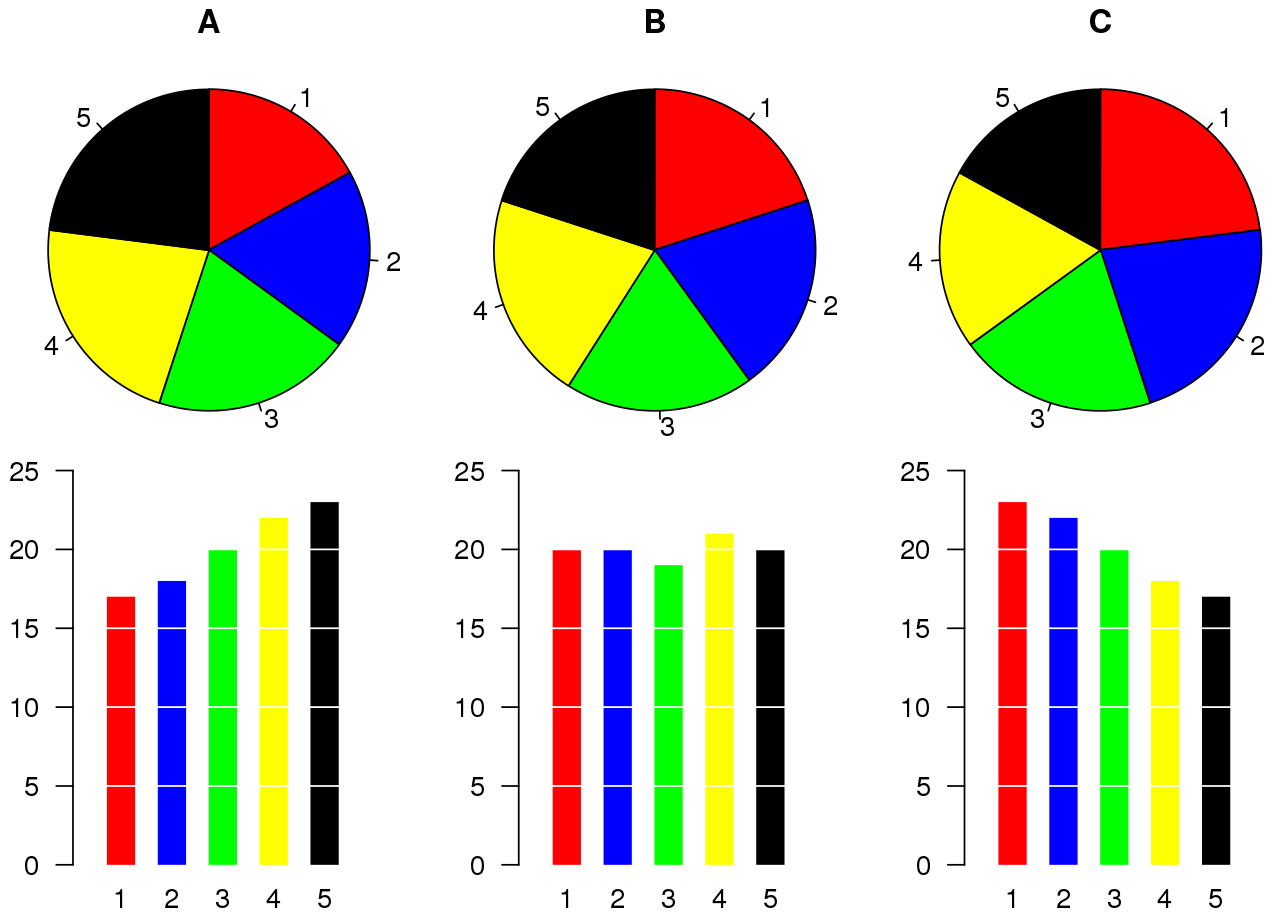
\includegraphics[width=.8\textwidth]{screen7.png}

\scriptsize\url{https://en.wikipedia.org/wiki/Misleading_graph}
\caption{Comparing Pie Charts}
\label{fig:comparingpies}
\end{figure}

	\item \emph{Graph unrelated data to suggest non-existent relationships.} The viewer of a visualization expects that data that is graphed together has a meaningful relationship. Simply by graphing data together, the analyst suggests a relationship where none may exist.
	\item \emph{Scale multiple vertical axes to suggest correlations.} Scaling a graph with multiple vertical axes so that lines better align shows visual similarities that are not borne out by the data.
	\item \emph{Use confusing colors.} For example, a color palette whose perceived color differences do not map linearly to the actual differences in the data may be misleading. For another example, using different shades of the same color for values that are very different will visually diminish the difference.
	\item \emph{Omit summary statistics.} For example, showing only the mean or median values, e.g. in a line or bar chart, omits the uncertainty in the data. It is better to also include error bars, information about quartiles or outliers in the chart to show variability or uncertainty, especially when there is significant uncertainty about differences or absolute values.
	\item \emph{Truncate or scale axes to hide or exaggerate trend.} Truncating or scaling axes leads to increased slopes of lines or perceived differences between points or levels. This exaggerates differences or trends. Figure~\ref{fig:truncated} shows an example of how small differences (right) can be exaggerated (left) in a bar chart. Similarly, Figure~\ref{fig:aspectratios} shows how scaling or the use of different aspect ratios can be used to visually exaggerate or diminish trends or relationships between variables.
\begin{figure}
\centering
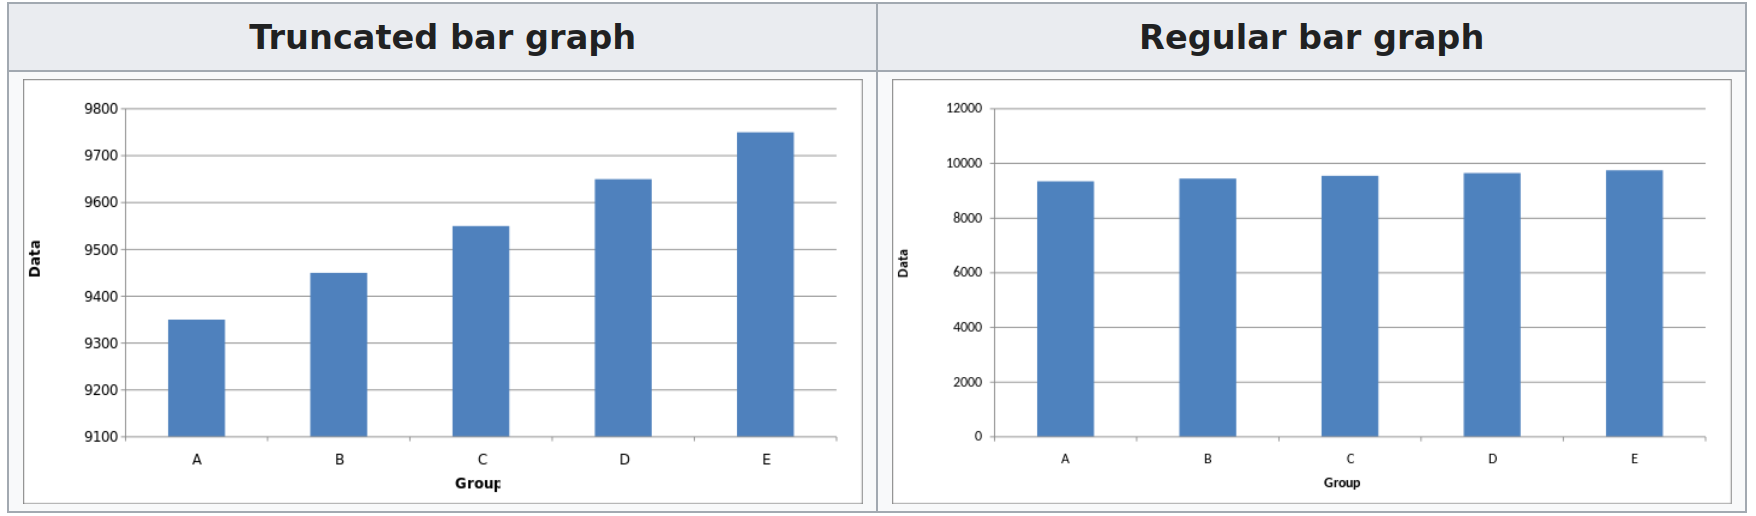
\includegraphics[width=.85\textwidth]{screen3.png} \\

\scriptsize\url{https://en.wikipedia.org/wiki/Misleading_graph}
\caption{Truncated Axes}
\label{fig:truncated}
\end{figure}
\begin{figure}
\centering
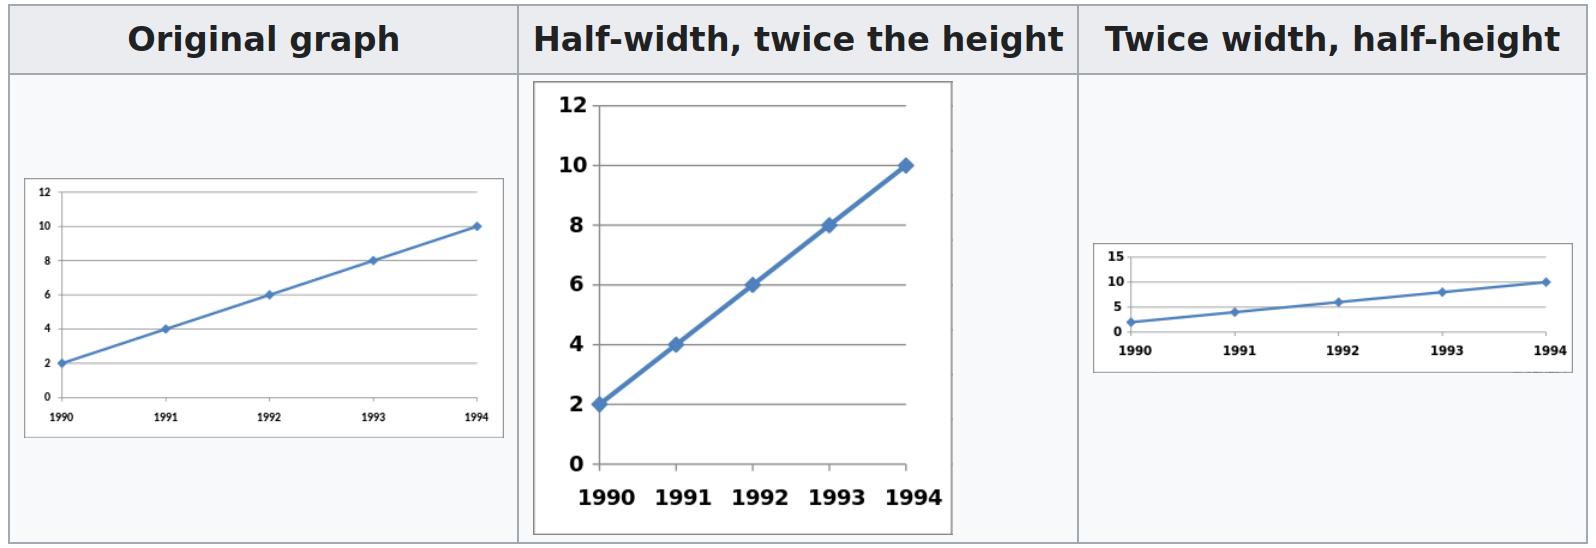
\includegraphics[width=\textwidth]{screen4.png}

\scriptsize\url{https://en.wikipedia.org/wiki/Misleading_graph}
\caption{Scaling Axes and Aspect Ratios}
\label{fig:aspectratios}
\end{figure}
	\item \emph{Scale in multiple dimensions.} The relative change or difference should be represented by a single dimension only. For example, in a bar or column chart, only the height or length of bar/column should change, not its width or area as well. This issue is often connected to the use of 3-dimensional graphics. While visually appealing, they exaggerate the apparent visual area of a foreground object, as illustrated in Figure~\ref{fig:3dpie}. A related issue is the use of images in graphs, shown in Figure~\ref{fig:imagesgraphs}. In the improper scaling, the image is enlarged in two dimensions, suggesting a larger difference than there actually exists in the data.
\begin{figure}
\centering
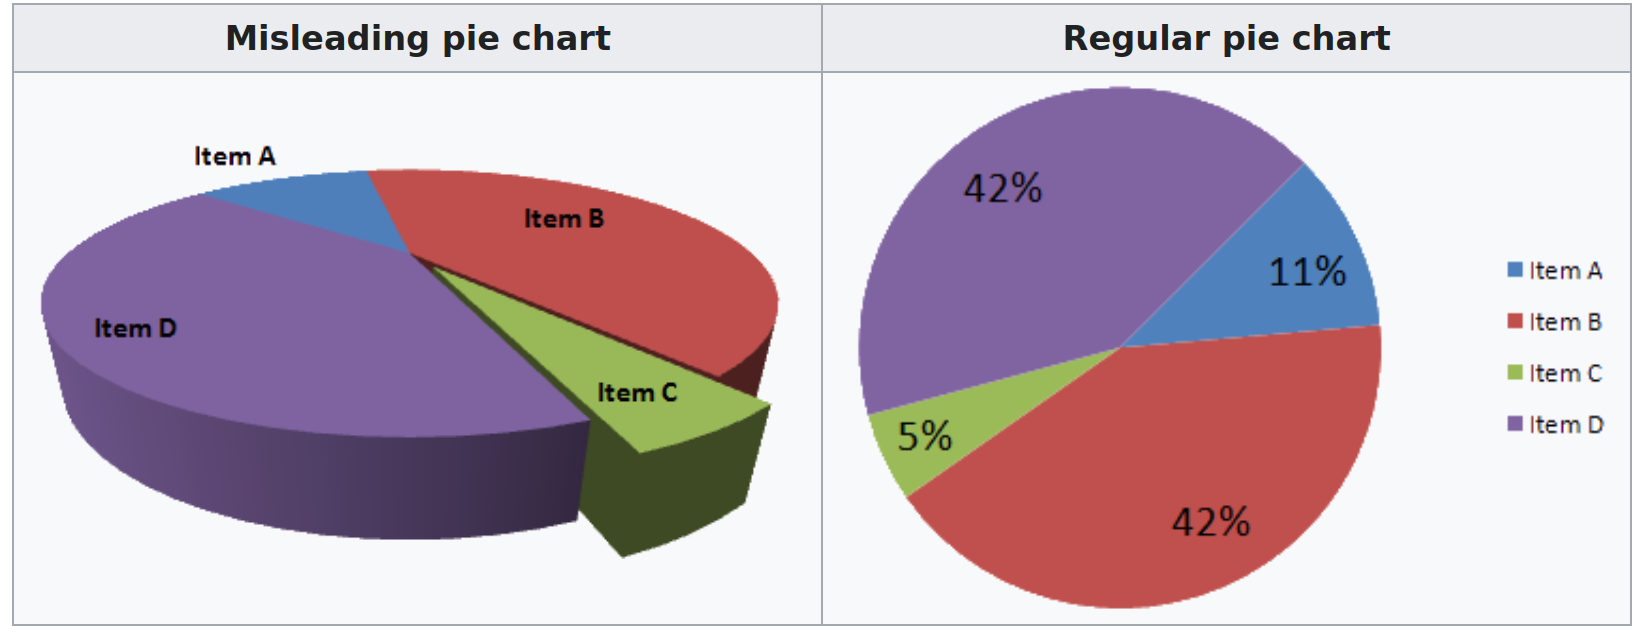
\includegraphics[width=.8\textwidth]{screen6.png}

\scriptsize\url{https://en.wikipedia.org/wiki/Misleading_graph}
\caption{3D Pie Charts}
\label{fig:3dpie}
\end{figure}
\begin{figure}
\centering
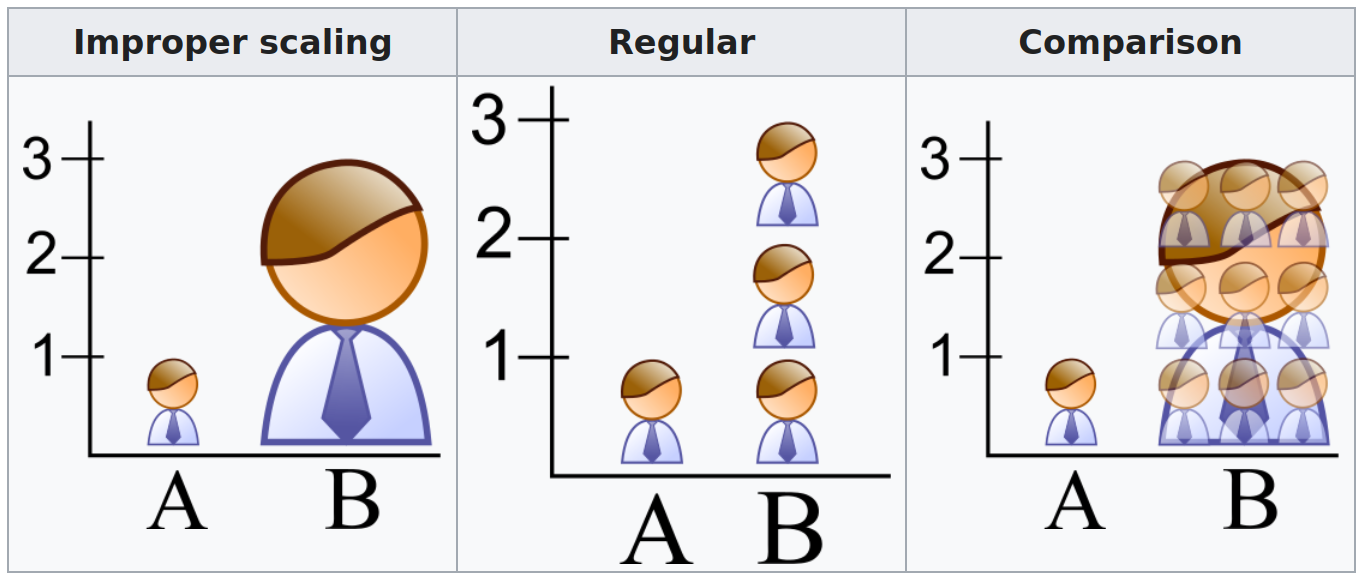
\includegraphics[width=.75\textwidth]{screen1.png}

\scriptsize\url{https://en.wikipedia.org/wiki/Misleading_graph}
\caption{Scaling Multiple Dimensions}
\label{fig:imagesgraphs}
\end{figure}
	\item \emph{Plot cumulative growth to hide trend.} A cumulative trend will always a positive trend, even as the contribution of individual items decreases sharply.
	\item \emph{Use maps for non-geographic data.} Maps represent geographical area, rather than population or some other variables of interest. For example, coloring a map by voter preference visually overemphasizes thinly populated but large geographic areas.
	\item \emph{Use incomplete data (''cherry-picking'')}. This includes examples such as showing only the previous year's data, instead of data for the previous five years to hide a trend, showing quarterly data instead of weekly data to hide volatility, or showing every data for every second month instead of for every month to hide specific data points or trends. Figure~\ref{fig:omitted} shows an example of this dark pattern.
	\item \emph{Use invalid data.} When data is known to be unreliable, that is, its quality is low, its uncertainty may be high, and it has a large error rate, it is misleading to use it to convey a quantitative message. 
\begin{figure}
\centering
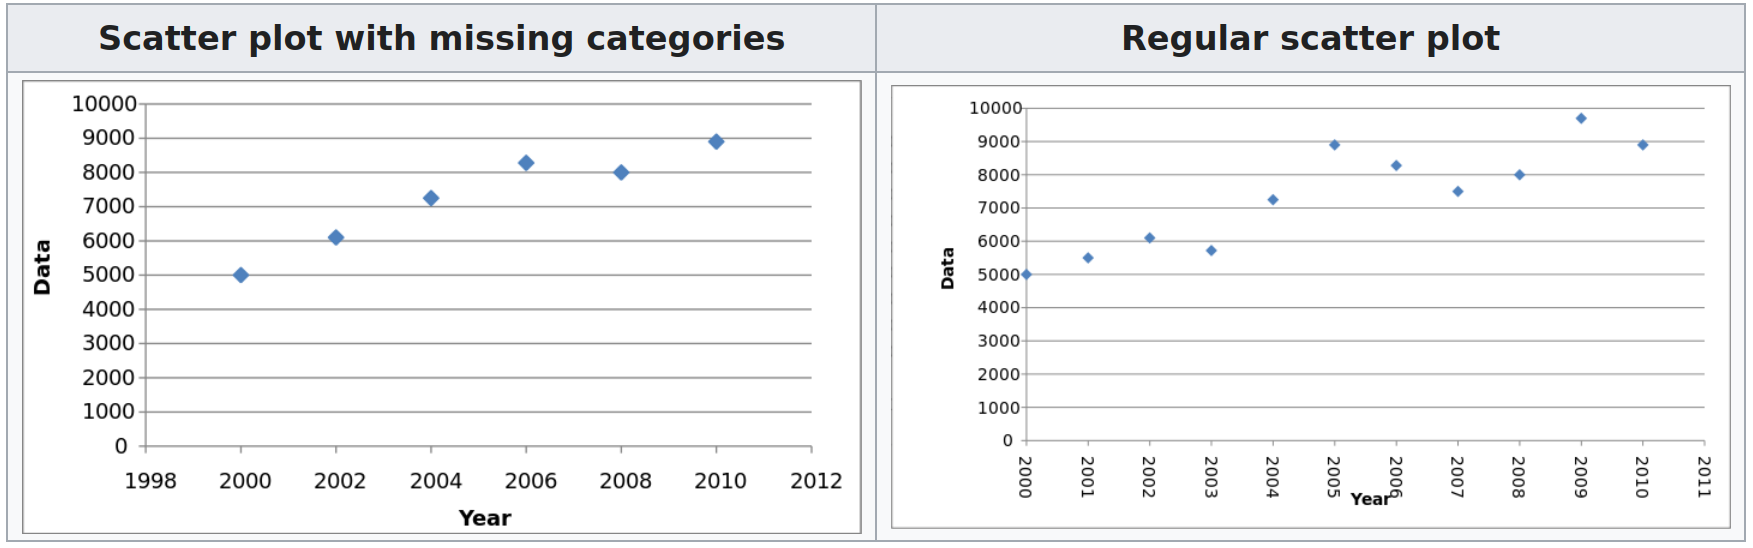
\includegraphics[width=\textwidth]{screen5.png}

\scriptsize\url{https://en.wikipedia.org/wiki/Misleading_graph}
\caption{Incomplete Data}
\label{fig:omitted}
\end{figure}

\end{itemize}	

The comics in Figure~\ref{fig:xkcd}, taken from the popular XKCD website\footnote{All XKCD comics are copyright by their creator (\url{www.xkcd.com}) and licensed under CC-BY-NC.} shows some of these visualization dark patterns in a humorous way. 

In summary, misleading charts and visualizations can be particularly problematic because they exploit the visual nature of human perception, making the deception less noticeable. It is crucial for both creators and consumers of data visualizations to be aware of these pitfalls and to approach data representation and interpretation with a critical eye.

\begin{figure}
\centering
\begin{subfigure}{.49\textwidth}
\centering
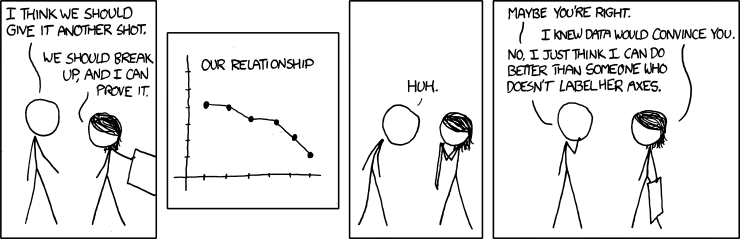
\includegraphics[width=\textwidth]{xkcd_convincing.png}
%\caption{Label your axes}
\end{subfigure}
\hfill
\begin{subfigure}{.49\textwidth}
\centering
  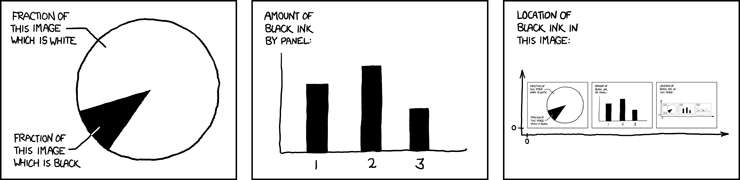
\includegraphics[width=\textwidth]{xkcd_self_description.png} 
%\caption{Use meaningful data}
\end{subfigure}
\hfill
\begin{subfigure}{.49\textwidth}
\centering
  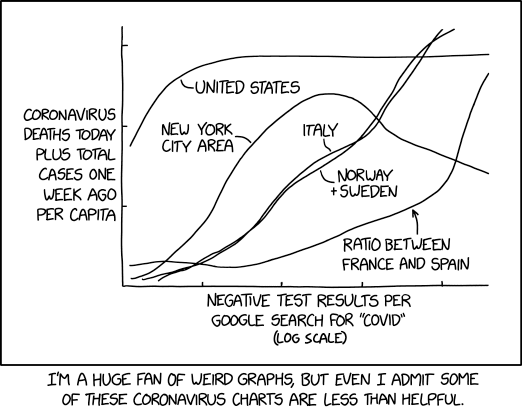
\includegraphics[width=\textwidth]{xkcd_coronavirus_charts.png}
%\caption{Use related data}
\end{subfigure}
\hfill
\begin{subfigure}{.49\textwidth}
\centering
  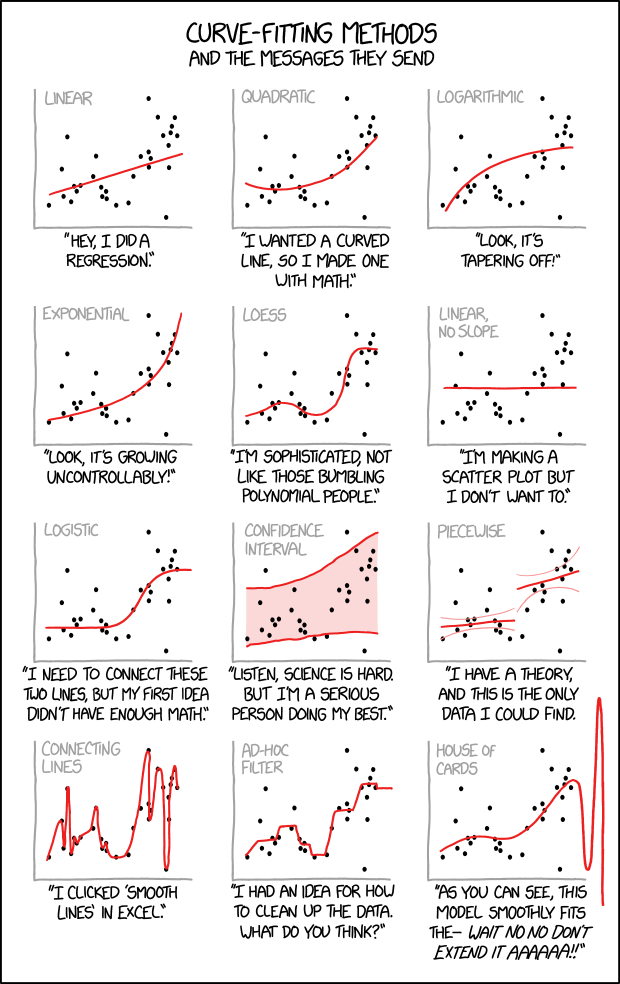
\includegraphics[height=3in]{xkcd_curve_fitting.png}
%\caption{Do not mislead}
\end{subfigure}
\hfill
\begin{subfigure}{.49\textwidth}
\centering
  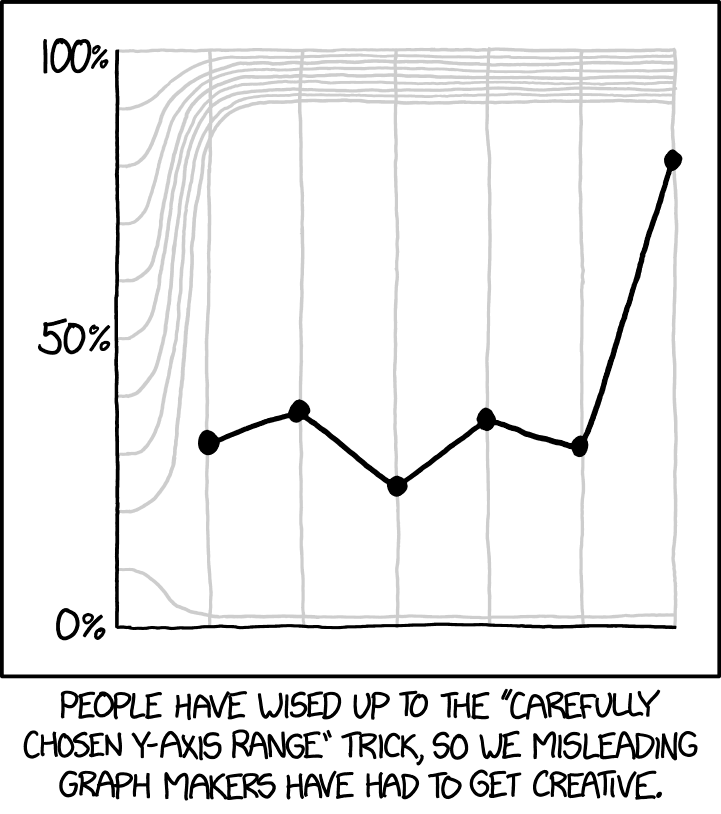
\includegraphics[height=2in]{xkcd_y_axis_2x.png}
%\caption{Choose Your Axes Meaningfully}
\end{subfigure}
\hfill
\begin{subfigure}{.49\textwidth}
\centering
  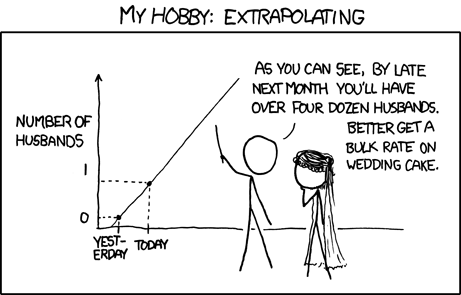
\includegraphics[width=.9\textwidth]{xkcd_extrapolating.png}
%\caption{Be Careful when extrapolating}
\end{subfigure}
\hfill
\begin{subfigure}{.49\textwidth}
\centering
  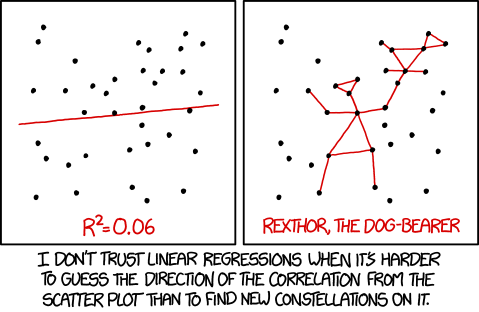
\includegraphics[width=\textwidth]{xkcd_linear_regression.png}
%\caption{Verify trends}
\end{subfigure}
\hfill
\begin{subfigure}{.49\textwidth}
\centering
  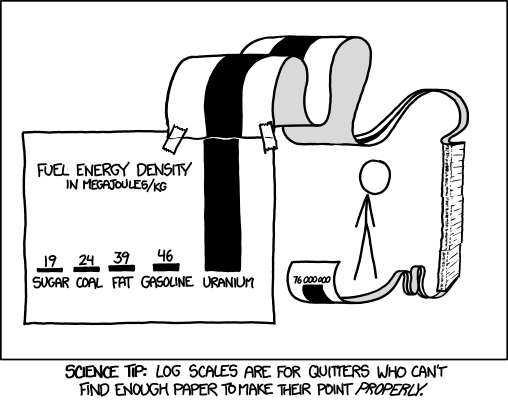
\includegraphics[width=.9\textwidth]{xkcd_log_scale.png}
%\caption{Use Appropriate Scales (XKCD)}
\end{subfigure}
 \\ 
\tiny \scriptsize{XKCD comics are copyright by their creator (\url{www.xkcd.com}) and licensed under CC-BY-NC}

\caption{Visualization Comics by XKCD}
\label{fig:xkcd}
\end{figure}


\section{Special Types of Data and Visual Analytics}

\subsection*{Streaming Data}

Visualizing streaming data, also known as real-time data visualization, involves the dynamic representation of data that is continuously updated as new data arrives. This type of visualization is essential in contexts where timely and rapid data interpretation is critical, such as in financial trading, or network monitoring. 

Streaming data presents some specific challenges for visualization. One of the primary challenges is managing the high velocity and volume of streaming data. The system must process and visualize data quickly enough to keep up with the incoming stream. Typically, only a limited window of data is available while older data is discarded. This means that, since the focus is on real-time data, it can be challenging to provide sufficient historical context for users to understand the current data in a broader temporal perspective. Moreover, due to the highly dynamic nature of the data, presenting streaming data in a way that is not overwhelming to the user is challenging. The visualization must strike a balance between providing enough detail and overloading the user with information, in particular information about changes, and between providing responsive graphs and overloading the user with such rapid changes they lose the ability to understand the data.

\subsection*{Spatial Data}

Visualizing geospatial or geographical data involves representing information that has a spatial component on a map or in a spatial context. While this type of visualization can be powerful for revealing patterns and insights related to location and geography, it presents some unique challenges. Geospatial data is often complex and multidimensional, encompassing not only locations but also attributes like time, elevation, population density, and more. Geospatial datasets can be very large, especially with the advent of satellite imagery, IoT (Internet of Things) sensors, and other sources of big data. Moreover, the granularity of physical space can range from very small areas of a few square meters to very large areas, such as provinces or states. For example, postal-code level data can produce very large data sets, even in small jurisdictions. 

A specific problem is the choice of areal unit to use for data analysis or visualization. For example, location data points can be aggregated by counties or districts, by postal code areas, by school districtcs or school intake areas, by police or fire service coverage, or many others. Each of these different areal units will lead to different data summaries and therefore also to different visualizations. Choosing the type of area to use as the basis for visualization can have a large impact on the insights gained or the messages conveyed to the audience. A simple example is shown in Figure~\ref{fig:maup} that shows how aggregate statistics depend on the type of areal unit or boundary.

\begin{figure}
\centering
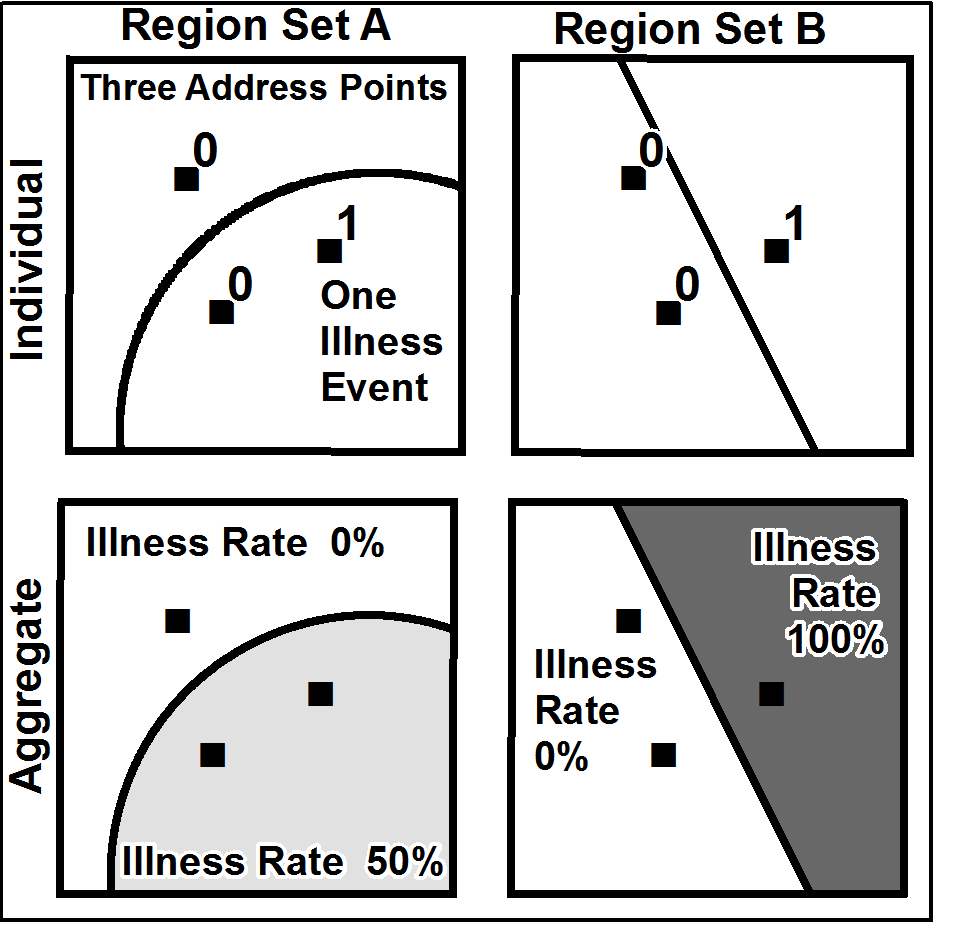
\includegraphics[width=.5\textwidth]{Maup_rate_numbers.png} \\

\small \url{https://en.wikipedia.org/wiki/File:Maup_rate_numbers.png}
\caption{Different types of spatial divisions lead to different interpretations} 
\label{fig:maup}
\end{figure}

Another particular challenge with spatial data is mapping the three-dimensional Earth onto a two-dimensional surface. This mapping inevitably involves some form of projection, which can distort spatial relationships. Choosing an appropriate map projection that minimizes distortion for the specific data and use case is a critical challenge. There are many such projections\footnote{\url{https://en.wikipedia.org/wiki/Map_projection}}, that distort or leave undistorted various properties such as lengths, areas, or angles. Figure~\ref{fig:xkcdmaps} shows some of these issues in a humorous way.

\begin{figure}
\centering
\begin{subfigure}{.49\textwidth}
\centering
  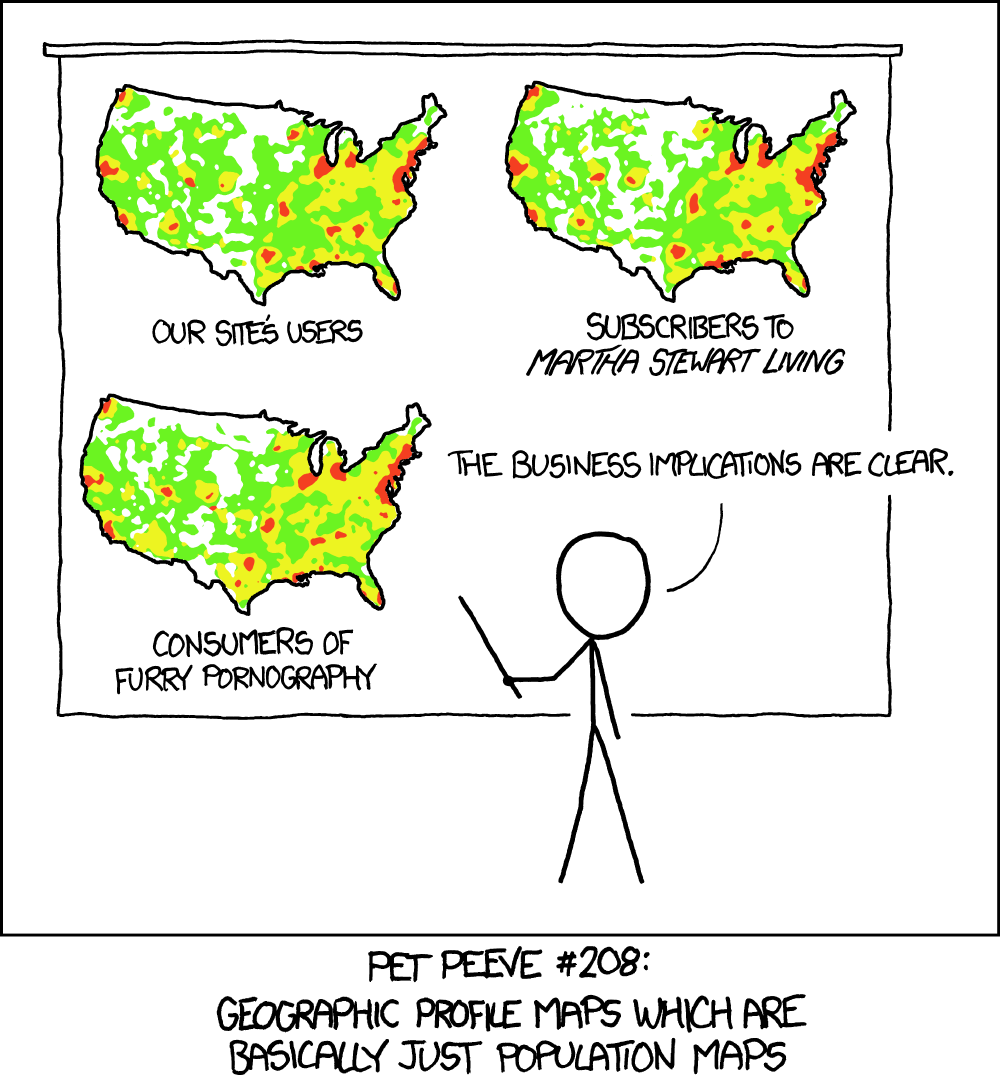
\includegraphics[width=\textwidth]{xdcd_heatmap_2x.png}
\end{subfigure}
\hfill
\begin{subfigure}{.49\textwidth}
\centering
  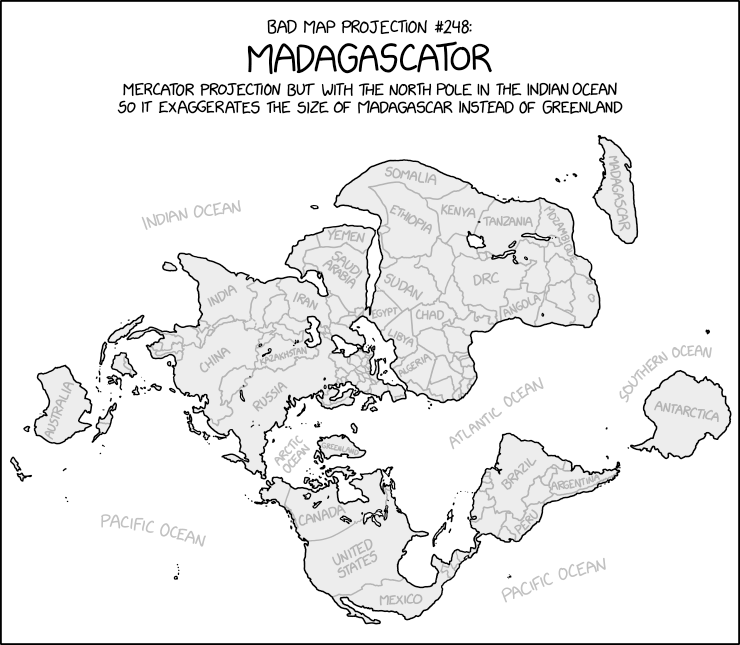
\includegraphics[width=\textwidth]{xkcd_bad_map_projection_madagascator.png}
\end{subfigure}
\hfill
\begin{subfigure}{.49\textwidth}
\centering
  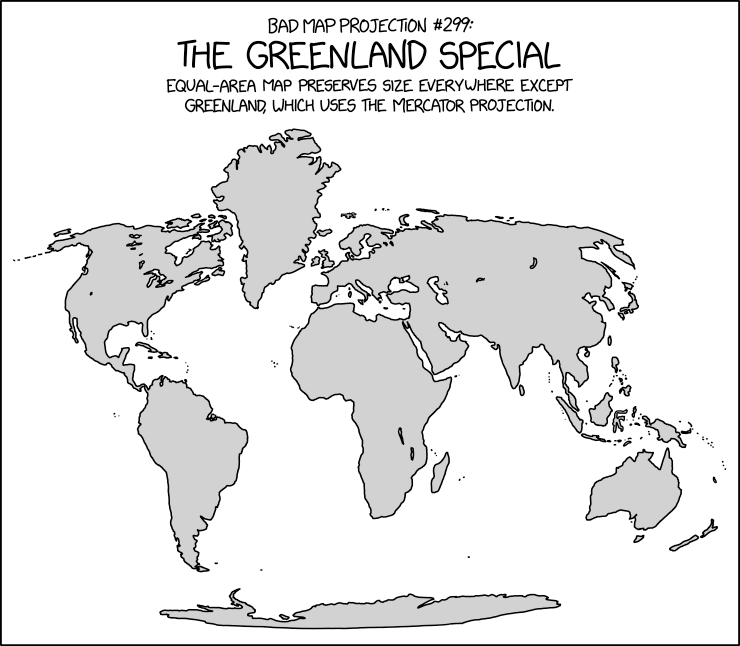
\includegraphics[width=\textwidth]{xkcd_bad_map_projection_the_greenland_special.png}
\end{subfigure}
\hfill
%\begin{subfigure}{.49\textwidth}
%\centering
  %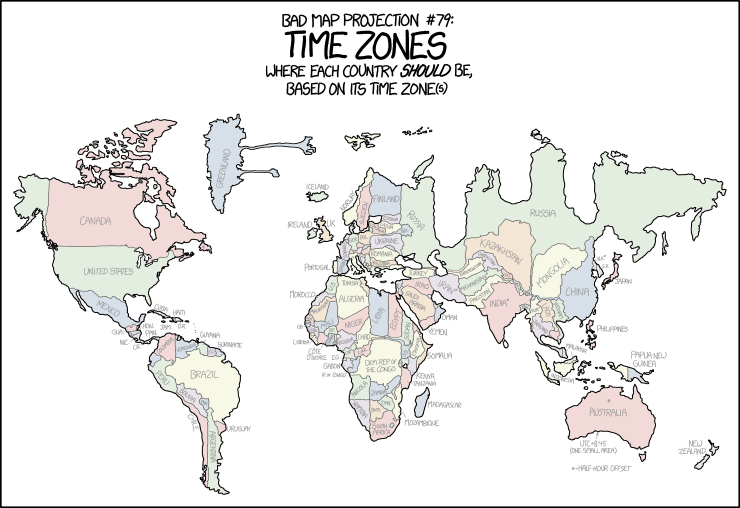
\includegraphics[width=\textwidth]{xkcd_bad_map_projection_time_zones.png}
%\end{subfigure}
%\hfill
\begin{subfigure}{.49\textwidth}
\centering
  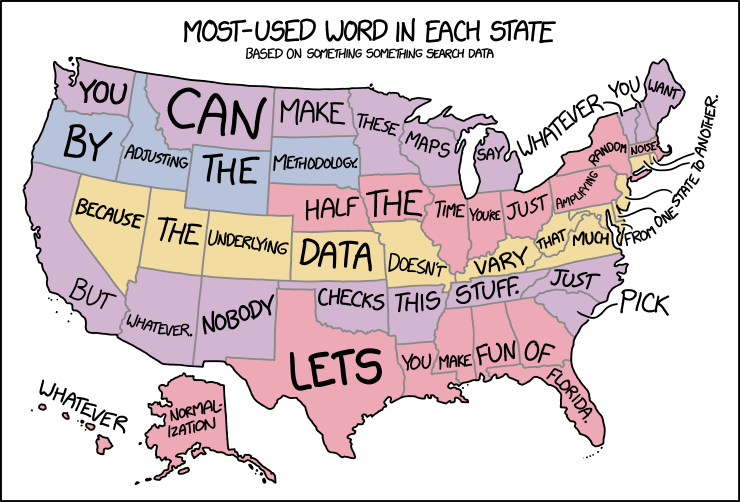
\includegraphics[width=\textwidth]{xkcd_state_word_map.png}
\end{subfigure} \\ 
\tiny \scriptsize{XKCD comics are copyright by their creator (\url{www.xkcd.com}) and licensed under CC-BY-NC}

\caption{Map Visualization Comics by XKCD}
\label{fig:xkcdmaps}
\end{figure}

\subsection*{Network and Graph Data}

Visualizing network or graph data involves representing entities as nodes and the relationships between them as edges in a graphical format. This type of visualization is crucial for understanding complex structures in various fields like social network analysis, biology, computer science, and more. Typically, nodes are represented as boxes, circles, or textual labels, while edges are represented as lines or curves. Directed graphs use arrowheads on lines or curves to indicate the directionality of an edge. 

Network visualization poses several unique challenges. Networks, especially large ones, can become very complex and cluttered when visualized. As the number of nodes and edges increases, the visualization can quickly become a tangled mess, making it difficult to discern meaningful patterns or relationships.

To effectively explore graph data, especially large graphs, interactive features like zooming, panning, and highlighting are essential. Finally, graphs often contain large sets of attributes for nodes and edges. Representing these attributes effectively without cluttering the visualization or overwhelming the viewer is challenging. Techniques like color coding, sizing, or shaping nodes and edges are commonly used but require careful design.

In densely connected networks, edges can overlap, and nodes can occlude each other, leading to a loss of information and making it difficult to trace relationships or identify individual elements. Choosing an appropriate layout algorithm is therefore crucial for network visualization. There exist many different ways to visually layout a graph to make it visually clear and easy to understand and generally of high quality. 

One of the most commonly-used types of algorithms position graph vertices based on physical metaphors of attractive and repulsive forces, for example an imaginary system of physical springs, sometimes called a force-directed graph layout\index{Force-directed graph layout}. Adjacent vertices are modelled with an attractive force, while all vertices have a repulsive force. The graph layout algorithm then tries to produce a layout in which an overall energy function is minimized. Figure~\ref{fig:sna_viz} shows an example of such a graph layout.

Another commonly used graph layout algorithm is the simple circular layout, where nodes are arranged equidistantly around a circle with edges drawn as lines or arrows. Figure~\ref{fig:circular} shows an example this type of graph layout.

In an arc diagram, as shown in Figure~\ref{fig:arc}, the nodes are arranged on a straight line while edges are drawn as semicircles between nodes. In this layout, it is important to arrange the nodes to minimize the number of crossings of edge semicircles. 

A common type of layout for directed and acyclic graphs is the layered graph, typically layed out from top to bottom or from left to right. The layout begins at the root node or nodes, and increments the layer for each edge between adjacent nodes, as shown in Figure~\ref{fig:layered}.

\begin{figure}
\centering
\includegraphics[width=.75\textwidth]{sna_viz.png} \\

\scriptsize \url{https://commons.wikimedia.org/wiki/File:SocialNetworkAnalysis.png}
\caption{Force-directed graph layout example} 
\label{fig:sna_viz}
\end{figure}

\begin{figure}
\centering
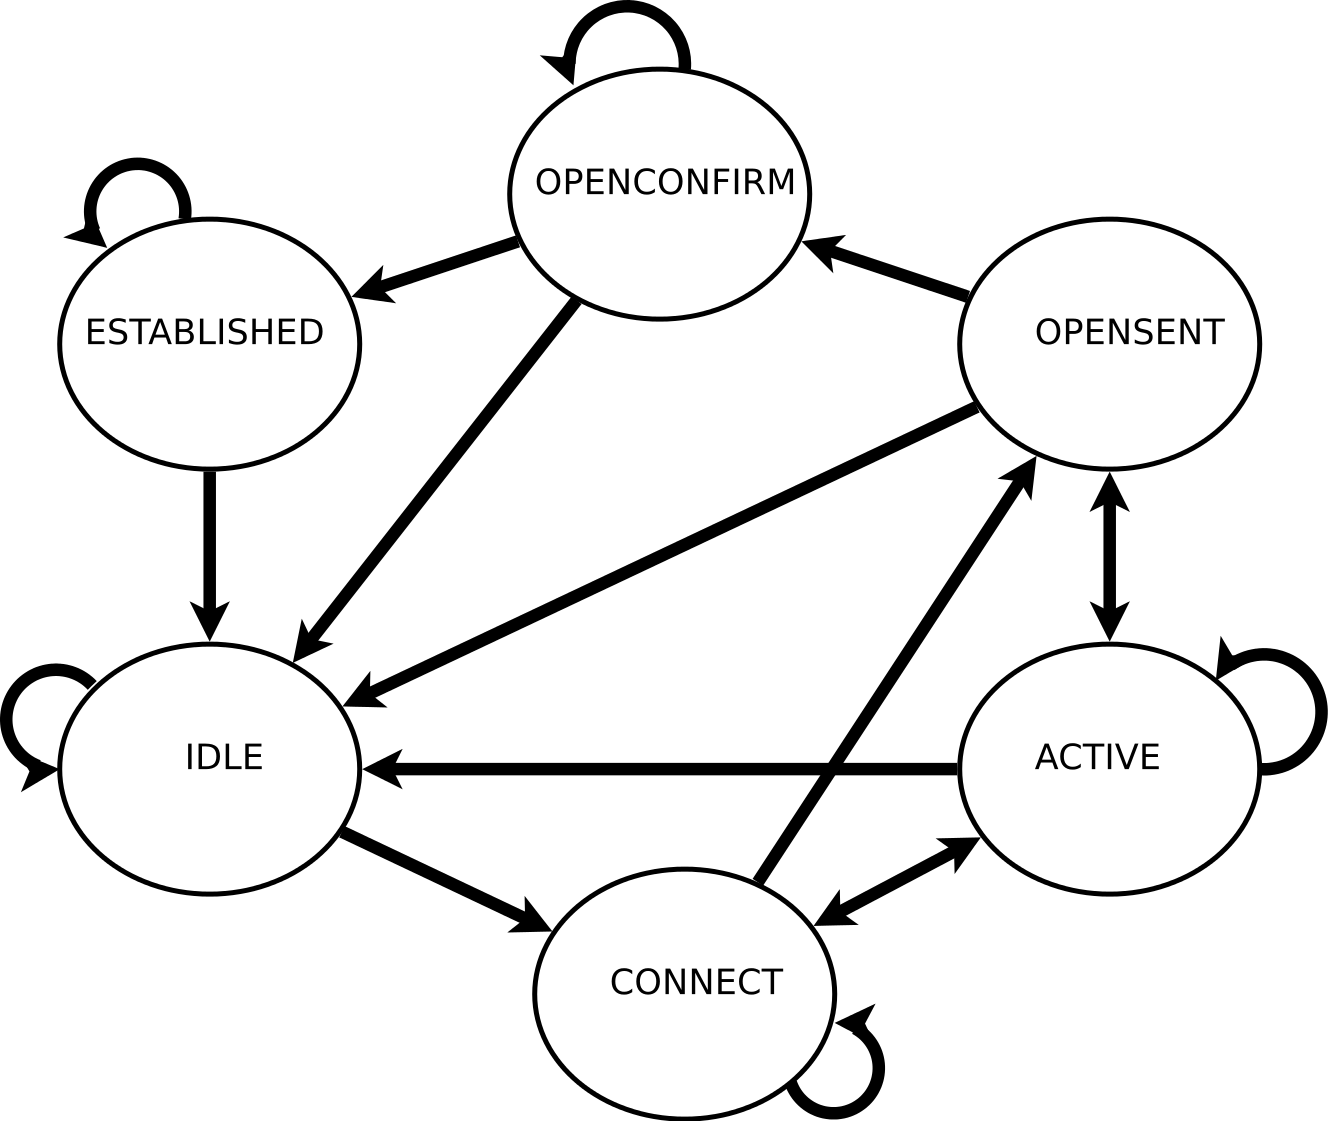
\includegraphics[width=.5\textwidth]{circular.png} \\

\scriptsize \url{https://commons.wikimedia.org/wiki/File:BGP_FSM_3.svg}
\caption{Circular graph layout example} 
\label{fig:circular}
\end{figure}

\begin{figure}
\centering
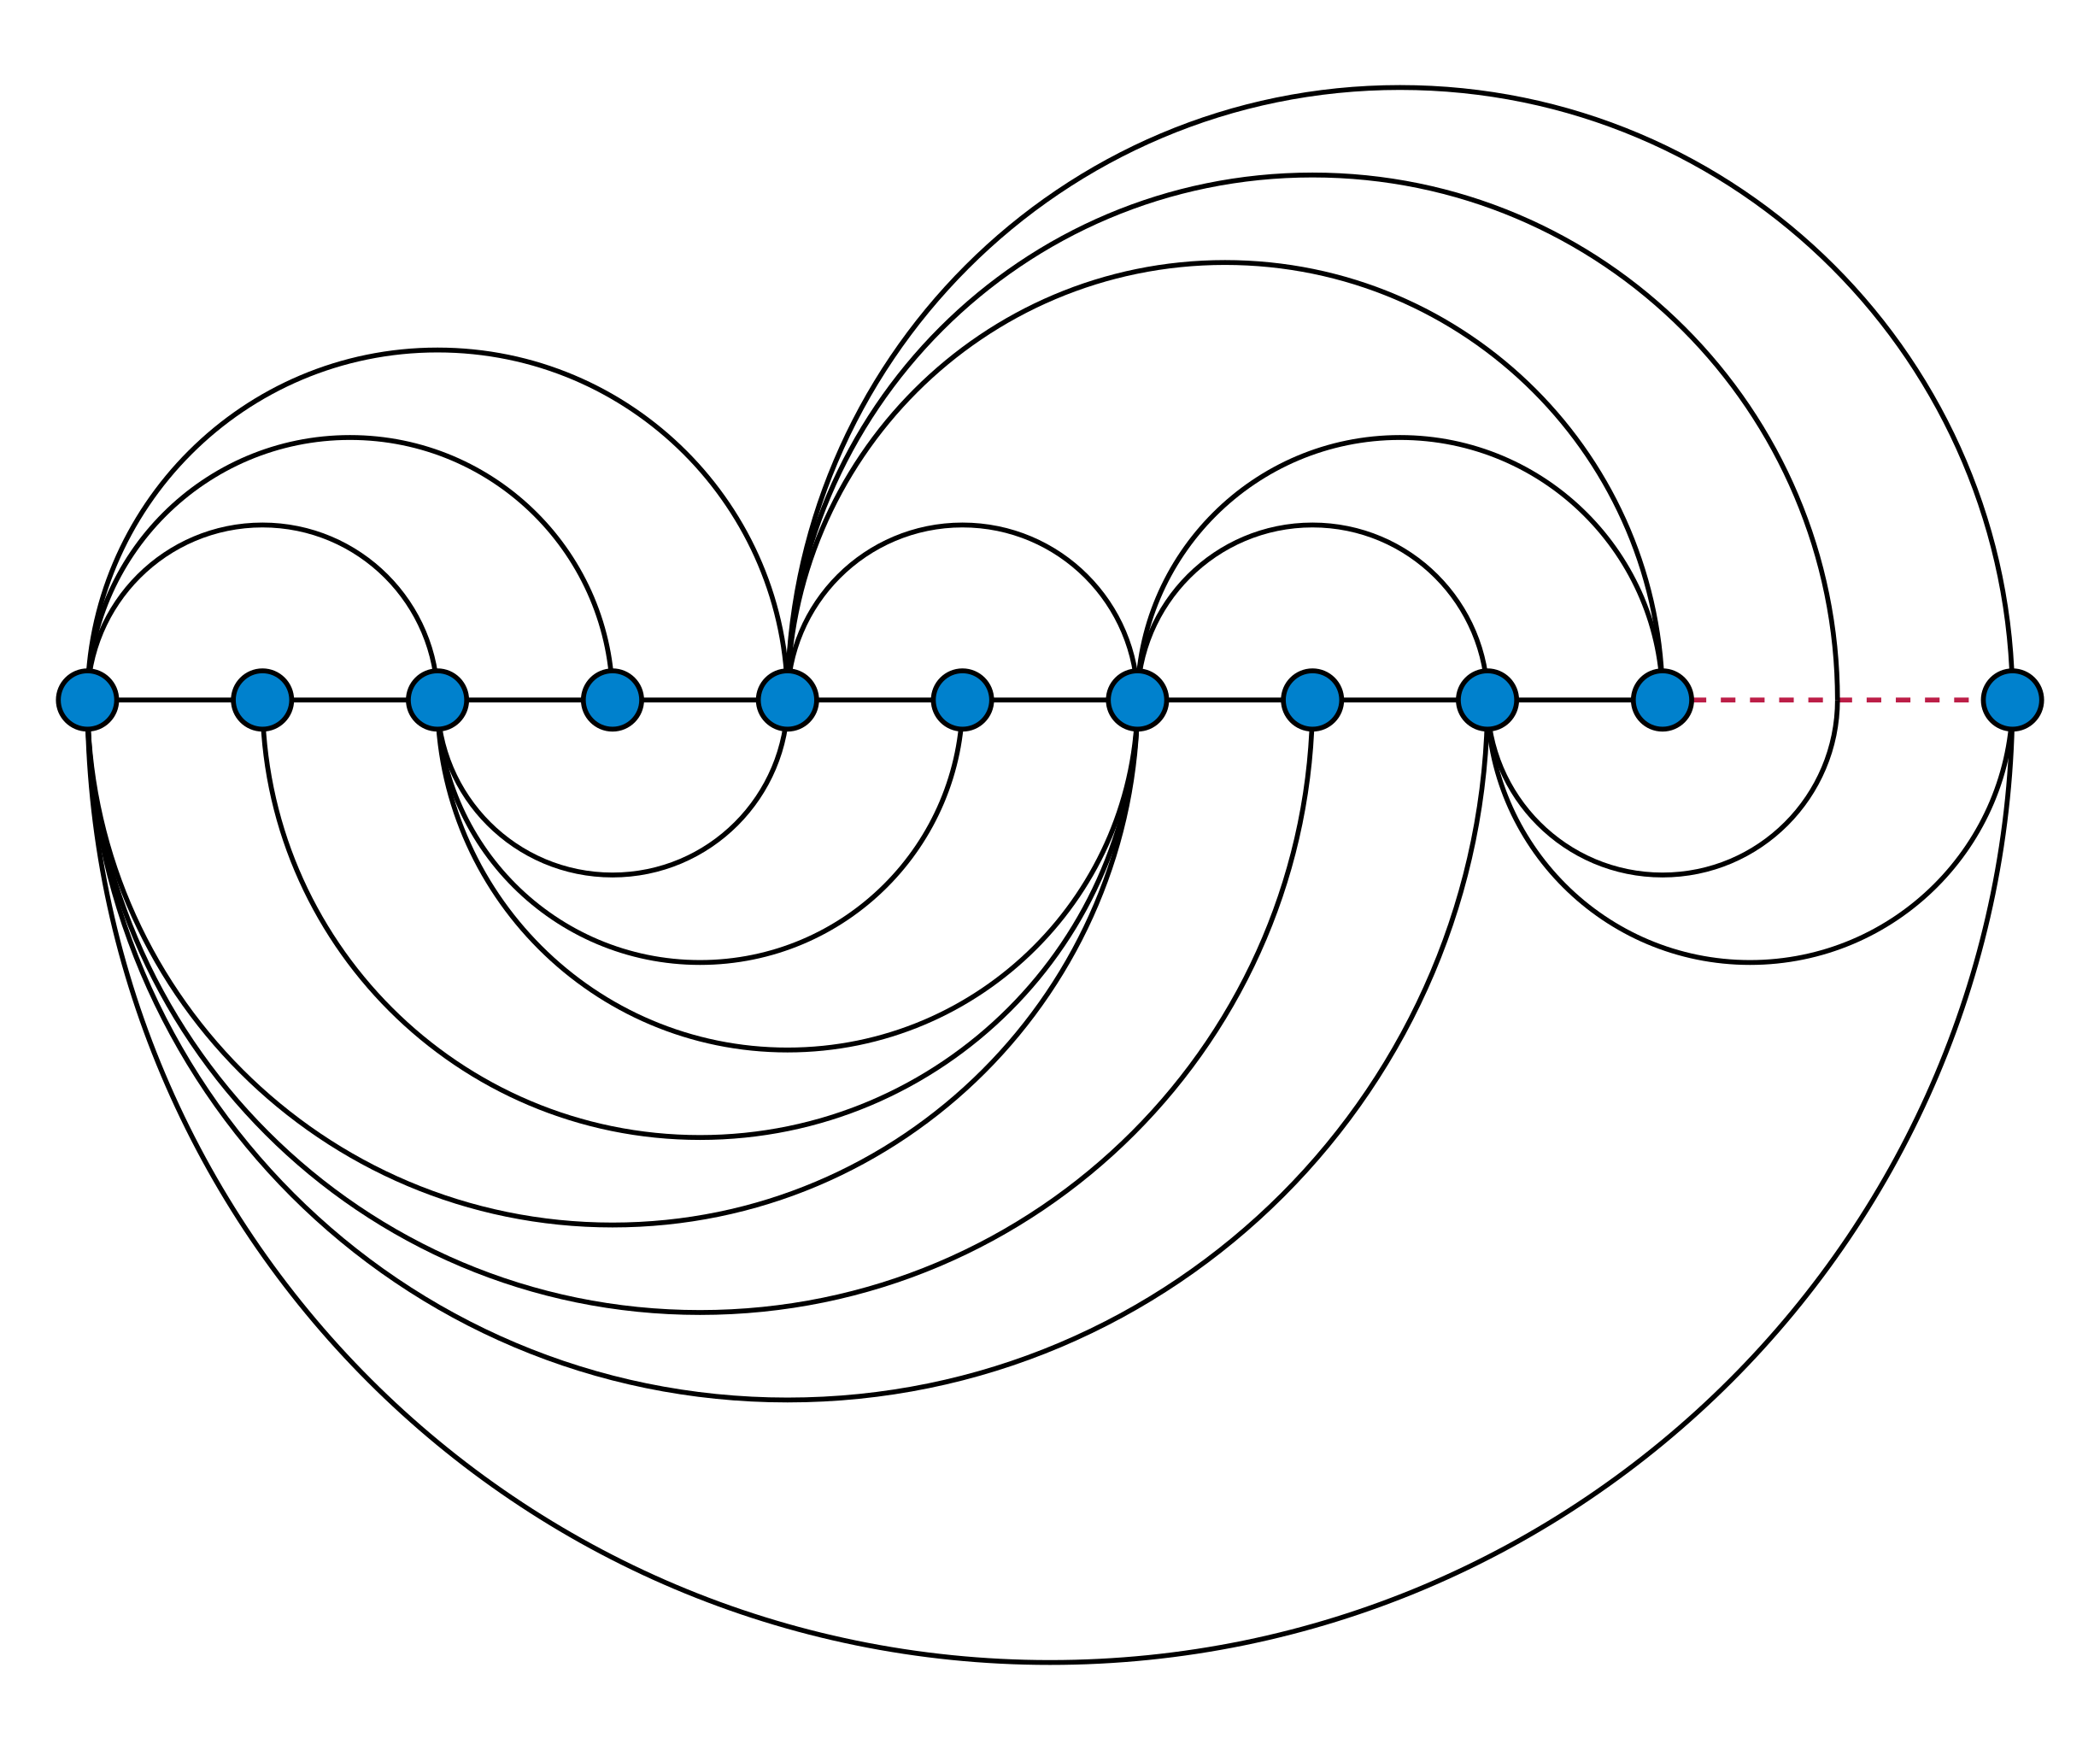
\includegraphics[width=.5\textwidth]{arc.png} \\

\scriptsize \url{https://commons.wikimedia.org/wiki/File:Goldner-Harary-linear.svg}
\caption{Arc graph layout example} 
\label{fig:arc}
\end{figure}

\begin{figure}
\centering
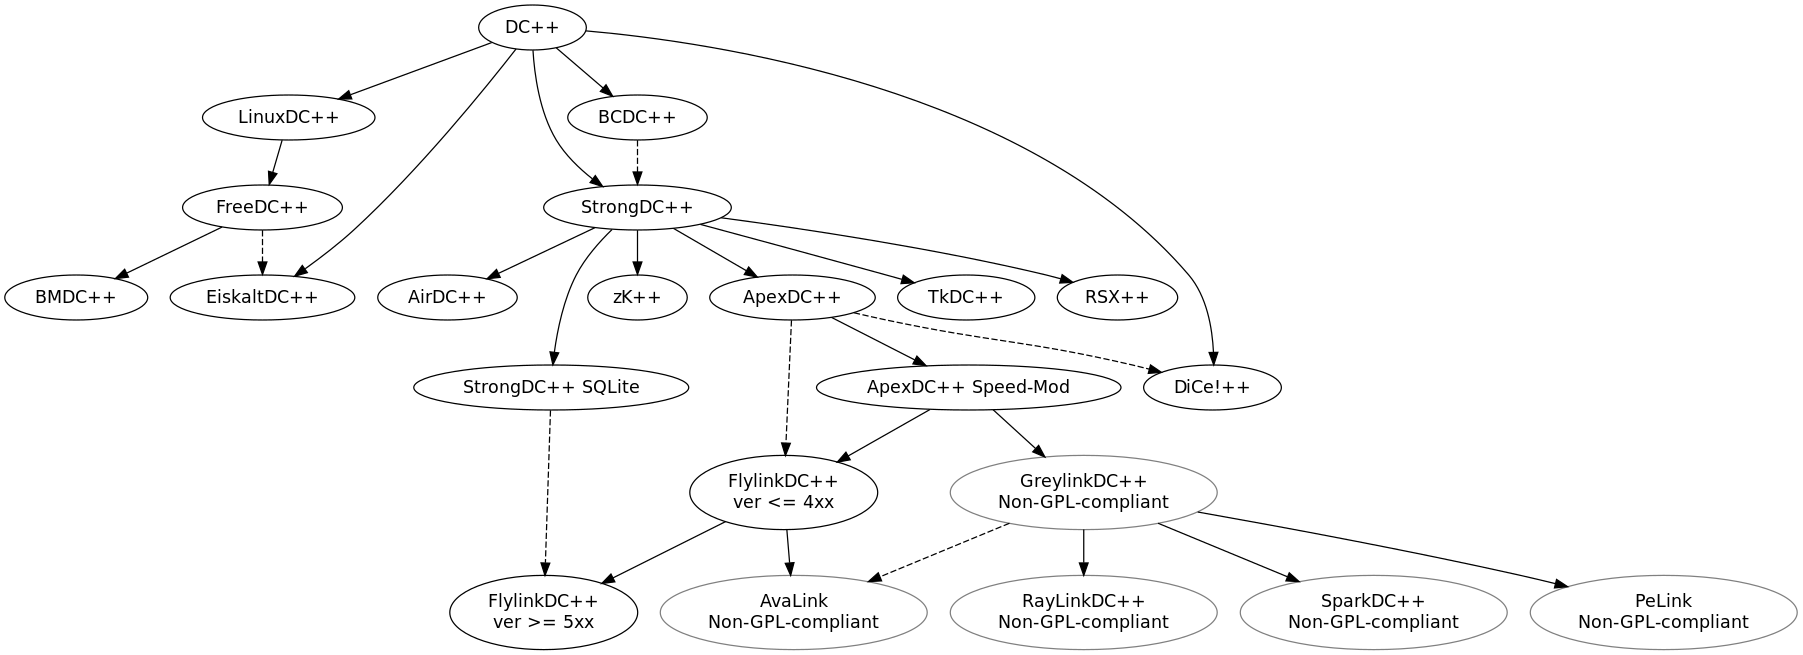
\includegraphics[width=\textwidth]{layered.png} \\

\scriptsize \url{https://commons.wikimedia.org/wiki/File:DC\%2B\%2B\_derivatives.svg}
\caption{Layered graph layout example} 
\label{fig:layered}
\end{figure}

\noindent When assessing the quality of the graph layout, a number of considerations are important:

\begin{itemize}
  \item \emph{Number of crossings of lines or curves}. Such crossings are visually confusing and should be minimized. In fact, this is such an important criterion that graph theory has defined a planar graph as one that can be visualized in two dimensions without any line crossings. Another qual
  \item \emph{Area of the graph}. Graphs should be drawn in the minimal amount of space while still being easy to read and understand.
  \item \emph{Symmetries}. Being able to exploit symmetries in the underlying graph data and represent or highlight them in the graphical layout makes the graph visualization easier to understand. 
  \item \emph{Shape homogeneity}. A particular problem when using node labels, e.g. for names or node attributes, is the size of the node shape in the graph visualization. It is preferrable to maintain equal size, despite differences in label length. Lines should have the lowest or an equal number of bends.
  \item \emph{Angular resolution}. In graphs with many edges from nodes, it is important to draw lines in such a way that the edges can be clearly differentiated. This is very important in circular layouts, but also plays a large role in other types of graph layouts.
\end{itemize}
  

\section{Color Palettes}

The use of color in data visualization is crucial, serving not only to enhance the visual appeal of a graphic but also to improve its clarity and interpretability. Color choices in data visualizations, determined by the selected color palettes, play a significant role in distinguishing different data points or categories, setting the tone of the presentation (for example, formal versus informal presentations), ensuring accessibility for viewers with color vision deficiencies, and enhancing the overall aesthetic appeal. Desirable characteristics of color palettes are:

\begin{itemize}
   \item \emph{Range of Values}: Colorful palettes are required when many different values have to be represented and distinguished.
   \item \emph{Perceptual Unformity}: The relative perceived differences between colors in the palette should mirror the relative differences in the data values represented by the colors.
   \item \emph{Robustness to Color Vision Deficiency}: Colour vision deficiency (CFD), colloquially called ''color blindness'' impacts almost 10\% of the population and must therefore be a consideration when choosing color palettes so that the data visualization can be properly perceived and interpreted by everyone.
   \item \emph{Consistency}: When using multiple plots, their color palette should be the same or at least consistent so as not to cause confusion in interpretation and require less effort for understanding by the reader.
   \item \emph{Aesthetic Appeal}: Finally, a colour palette should also be ''pretty''.
\end{itemize}

\subsection*{Types of Color Palettes}

Color palettes can be distinguished by the number of colours they use, and whether the colors span a continuous color space or are a discrete set. 

\subsubsection*{Sequential color palettes}

Sequential color palettes\index{Colour palette!sequential}, like the one in Figure~\ref{fig:sequential}, use a single color and vary the hue or depth of the color. They are best used for data that has an inherent order, as they clearly show progression or gradation. However, they are not suitable for data that lacks a natural ordering. The \emph{monochromatic color palette} is a special case of a sequential palette. This may be suitable when it is likely that the output will be printed on media without the use of color. 

\subsubsection*{Diverging color palettes}

Diverging color palettes\index{Colour palette!diverging}, like the one in Figure~\ref{fig:diverging}, on the other hand, use two colors as anchors and use gradations either through white, as in Figure~\ref{fig:diverging}, or through black. They are ideal for emphasizing deviations from a median or mean value, or for highlighting extremes on either side of a critical midpoint. However, these palettes may be misleading if used for data without a meaningful center.

\subsubsection*{Spectral color palettes}

Spectral color palettes\index{Colour palette!spectral}, like the one in Figure~\ref{fig:spectral} use a variety of different colors without any implicit ordering. They are used to represent discrete categories without inherent ordering, and are useful for differentiating distinct groups of data. The downside is that they can become confusing with too many categories. 

Sequential and diverging color palettes may be \emph{discrete}\index{Colour palette!discrete}, like the ones shown in Figure~\ref{fig:palettes}, or \emph{continuous}\index{Colour palette!continuous}, while spectral palettes are always discrete.

\begin{figure}
\begin{subfigure}{\textwidth}
\centering
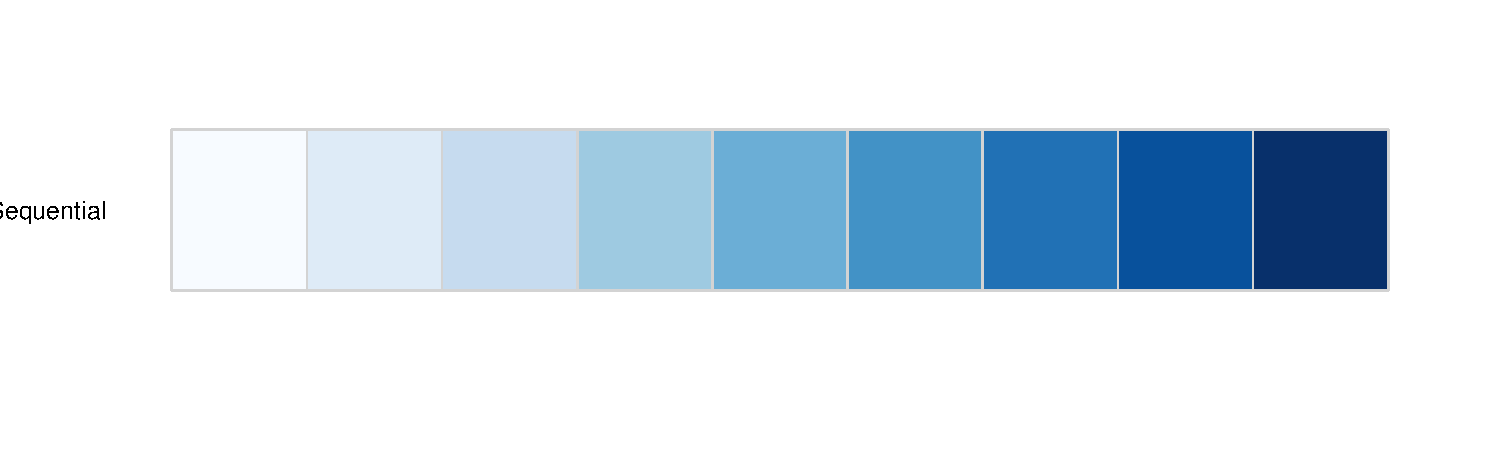
\includegraphics[width=.8\textwidth]{sequential.pdf}
\caption{Sequential color palette} 
\label{fig:sequential}
\end{subfigure}

\begin{subfigure}{\textwidth}
\centering
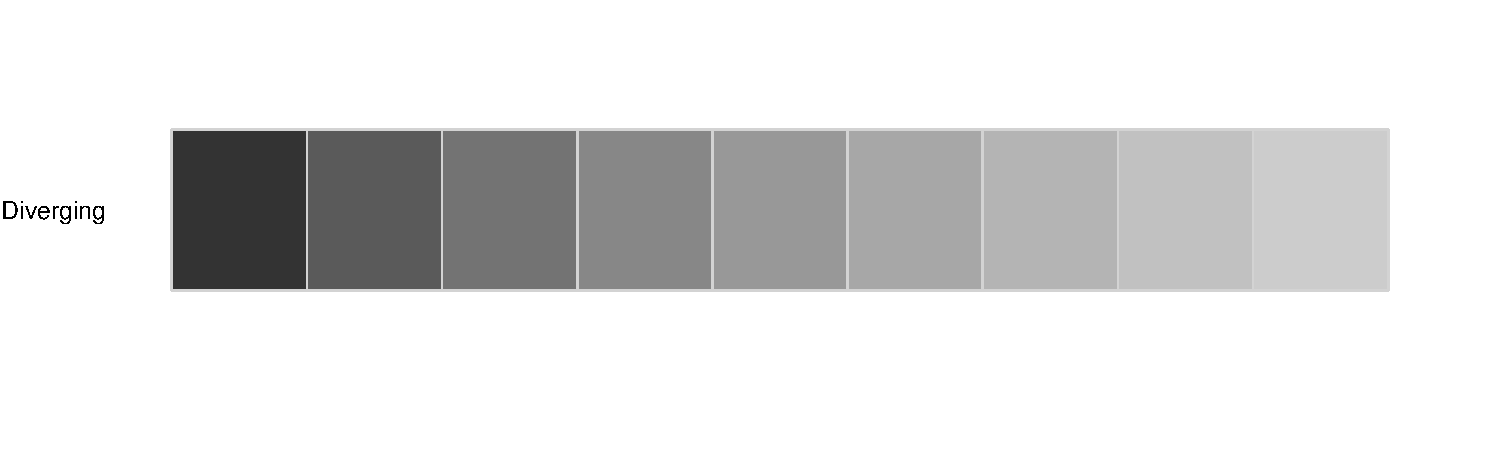
\includegraphics[width=.8\textwidth]{monochromatic.pdf}
\caption{Monochromatic color palette} 
\label{fig:monchromatic}
\end{subfigure}

\begin{subfigure}{\textwidth}
\centering
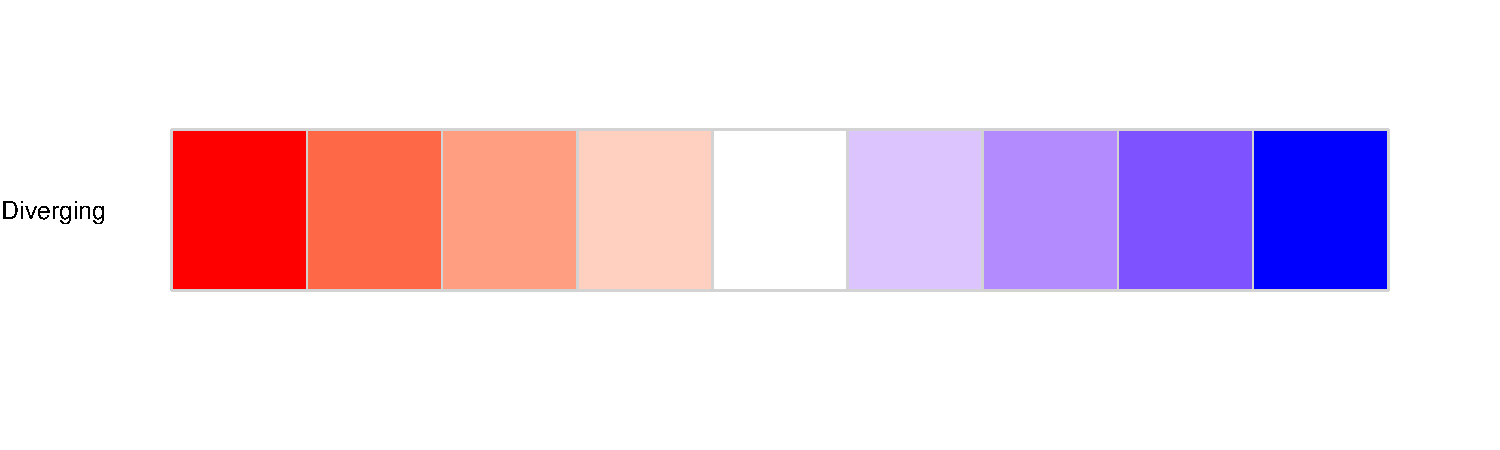
\includegraphics[width=.8\textwidth]{diverging.pdf}
\caption{Diverging color palette} 
\label{fig:diverging}
\end{subfigure}

\begin{subfigure}{\textwidth}
\centering
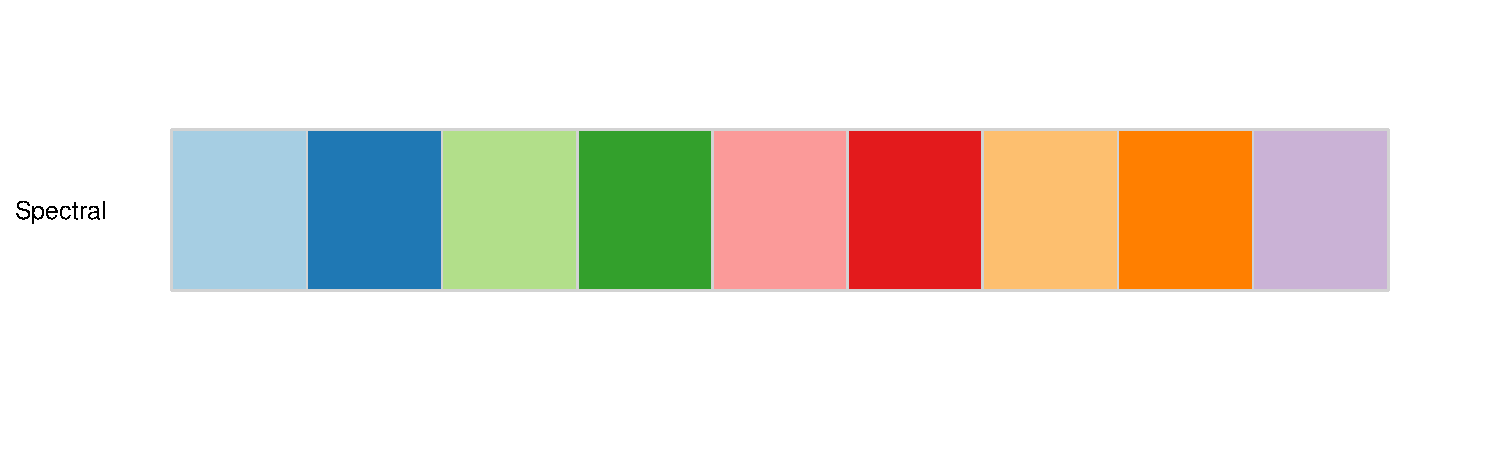
\includegraphics[width=.8\textwidth]{brewer.paired.pdf}
\caption{Spectral color palette} 
\label{fig:spectral}
\end{subfigure}

\caption{Types of Color Palettes}
\label{fig:palettes}
\end{figure}

\subsection*{Color Vision Deficiency}

The human eye contains three different types of color receptor cells, called ''S-cones'' that perceive the color blue, ''M-cones'' that perceive the color green, and ''L-cones'' that perceive the color red. Color vision deficiency (CVD)\index{Colour vision deficiency}\index{CVD|see{Colour vision deficiency}} is a biological impairment where some color receptor cells in the eye are missing, less frequent, or their function is diminished. In \emph{protanopia}\index{Protanopia}, the S-cones are missing or impaired, in \emph{deuteranopia}\index{Deuteranopia}, the M-cones are missing or impaired, and in \emph{tritanopia}\index{Tritanopia}, the L-cones are impaired. When all are missing or non-functional, one speaks of \emph{monochromatism}\index{Monochromatism}. CVD is a fairly common disability, afflicting approximately 1 in 12 men and 1 in 200 women, with an overall incidence rate in Canada of more than 5\%.

To show the different types of color deficiencies, consider the images in Figure~\ref{fig:cvd}. Figure~\ref{fig:cvd1} shows the original image as it is perceived by a person who does not suffer from CVD. The remaining four images show how the photo appears to persons with different types of CVD.

\begin{figure}
\centering
\begin{subfigure}{.75\textwidth}
\centering
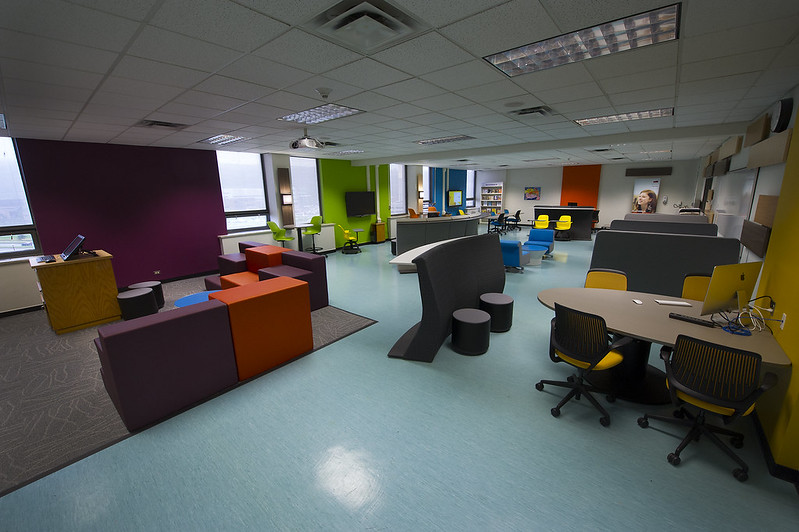
\includegraphics[width=\textwidth]{photo.jpg} \\

\scriptsize Copyright Memorial University of Newfoundland 
\caption{Original Image (MUN Faculty of Education Class Room)} 
\label{fig:cvd1}
\end{subfigure}
\hfill
\begin{subfigure}{.49\textwidth}
\centering
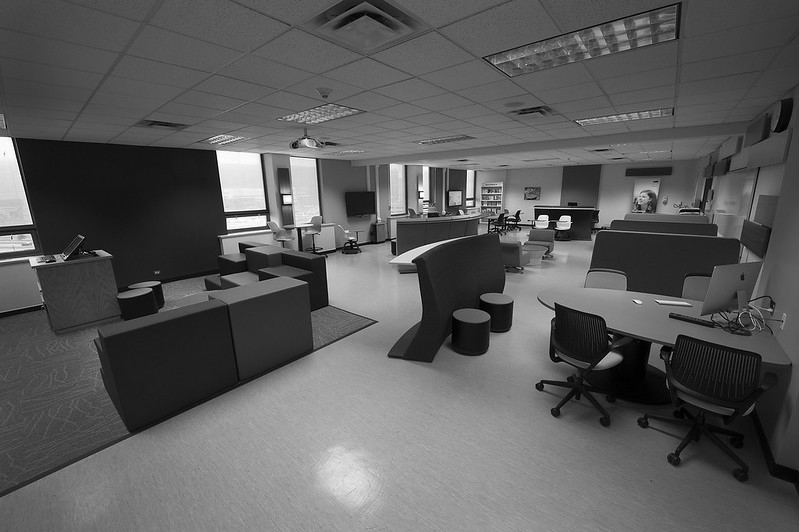
\includegraphics[width=\textwidth]{desaturate_photo.jpg}
\caption{Monochromatism} 
\label{fig:cvd2}
\end{subfigure}
\hfill
\begin{subfigure}{.49\textwidth}
\centering
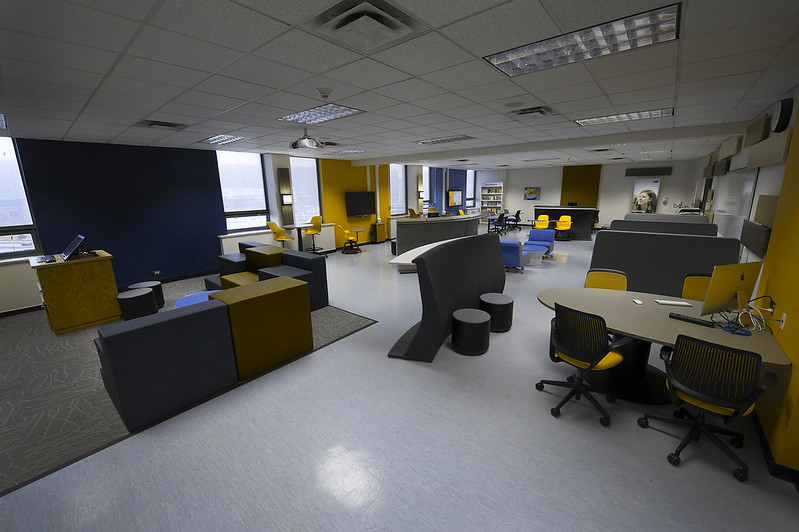
\includegraphics[width=\textwidth]{protan_photo.jpg}
\caption{Protanopia} 
\label{fig:cvd3}
\end{subfigure}
\hfill
\begin{subfigure}{.49\textwidth}
\centering
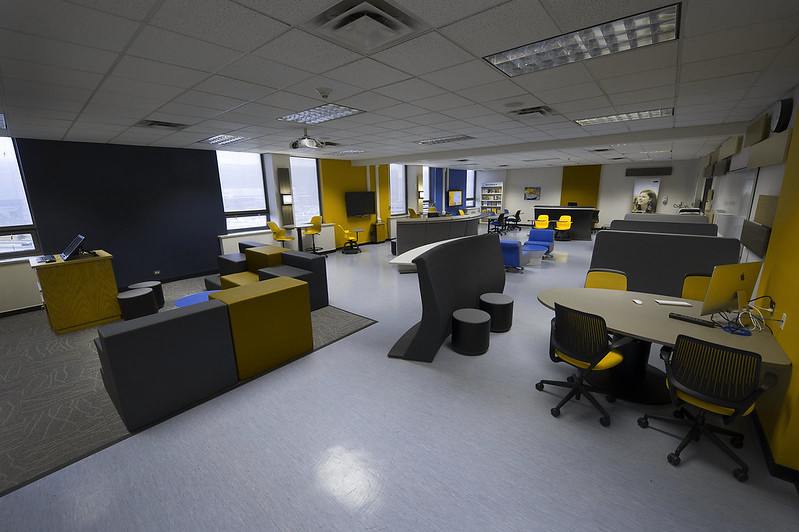
\includegraphics[width=\textwidth]{deutan_photo.jpg}
\caption{Deuteranopia} 
\label{fig:cvd4}
\end{subfigure}
\hfill
\begin{subfigure}{.49\textwidth}
\centering
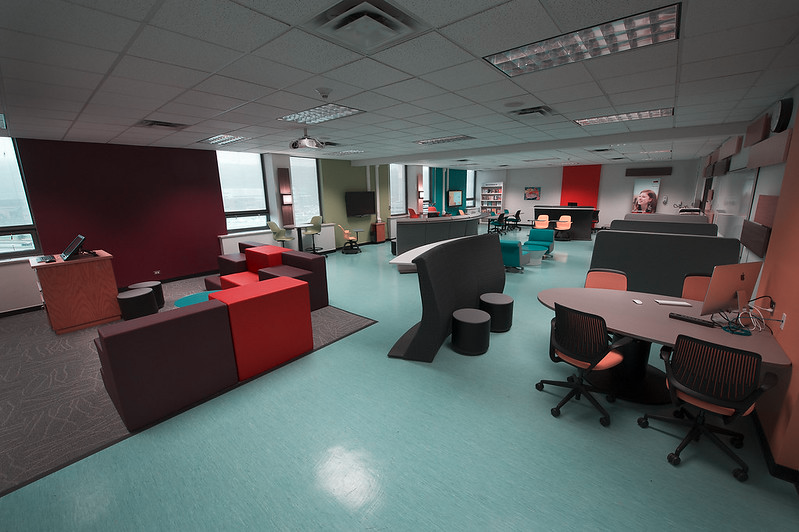
\includegraphics[width=\textwidth]{tritan_photo.jpg}
\caption{Tritanopia} 
\label{fig:cvd5}
\end{subfigure}
\hfill
\caption{Simulated Color Vision Deficiencies}
\label{fig:cvd}
\end{figure}

Realizing the prevalence and the effects of CVD means that the color palette that is chosen for data visualization should be interpretable for and lead to the same interpretation even for readers with CVD. For example, the Viridis color palette available in many visualization software packages was designed with CVD readability in mind. Compare the popular ''Color Brewer Paired'' palette in Figure~\ref{fig:paired} to the Viridis palette in Figure~\ref{fig:viridis}. The figures show that the Viridis palette is readable and interpretable with any CVD condition, whereas the Paired palette is not because some colors cannot be distinguished under various CVD conditions.

\begin{figure}
\centering
  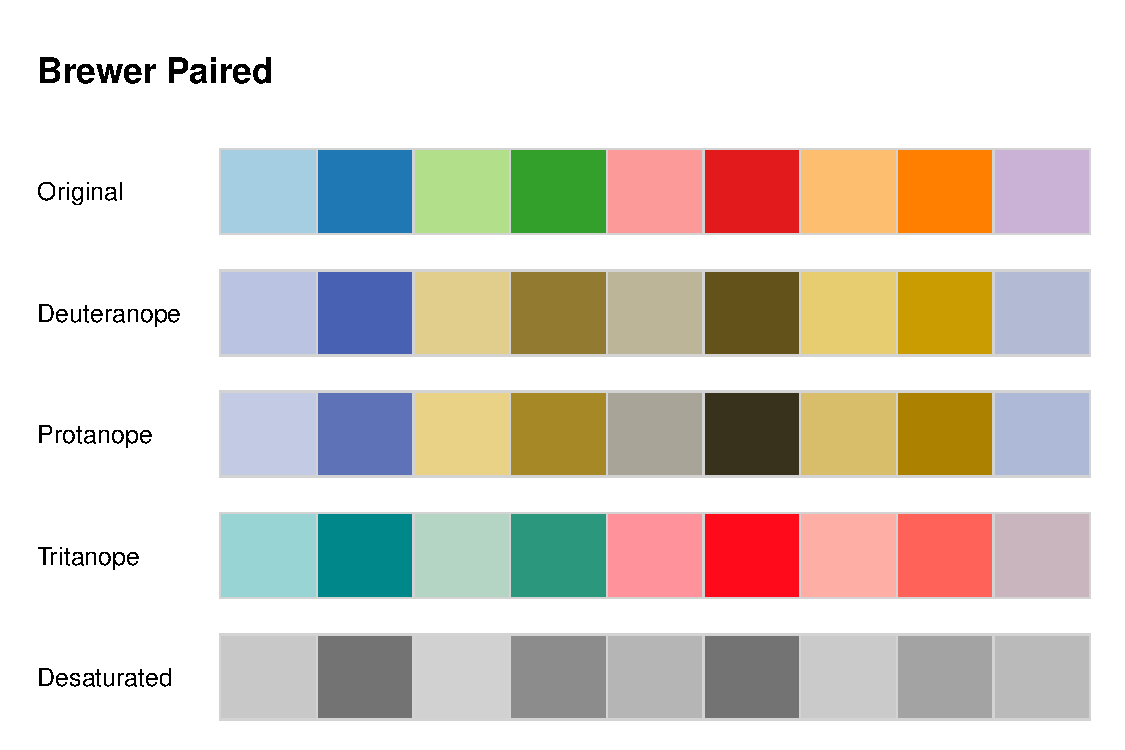
\includegraphics[width=.75\textwidth]{brewer.paired.cvd.pdf}

\caption{Example: Colourbrewer Palette ''Paired''}
\label{fig:paired}
\end{figure}

\begin{figure}
\centering
  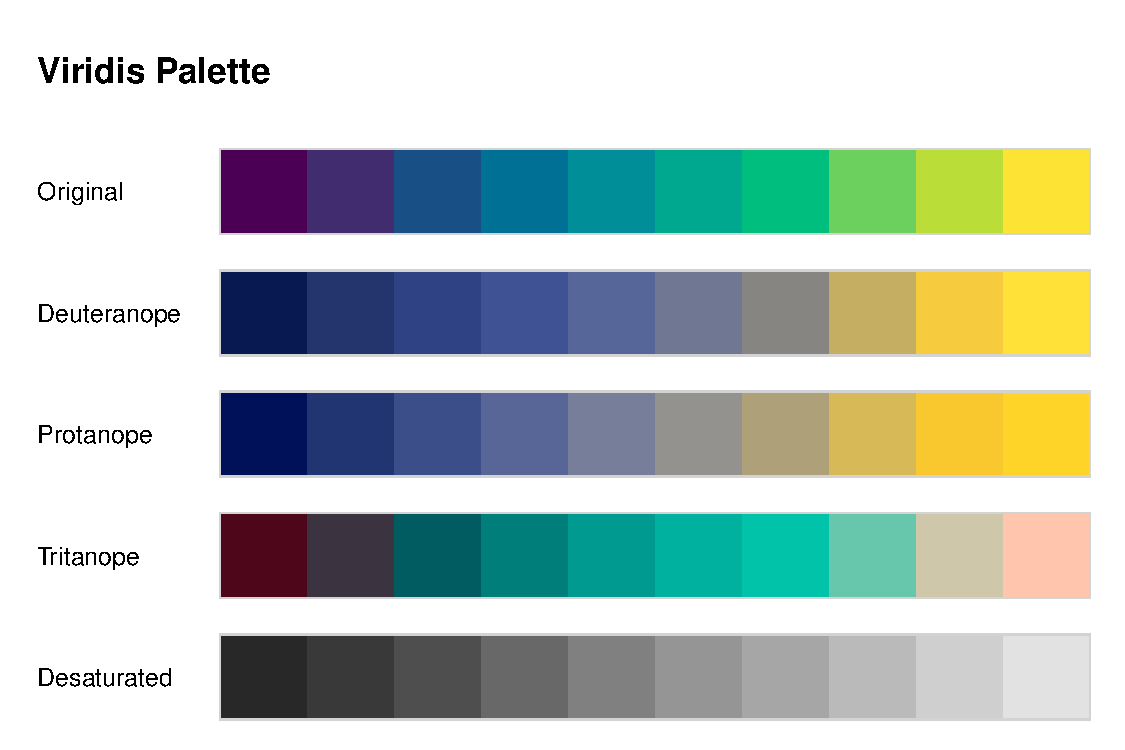
\includegraphics[width=.75\textwidth]{viridis.plot.pdf}

\caption{Viridis Colour Palette}
\label{fig:viridis}
\end{figure}

In summary, the thoughtful application of color in data visualization is not merely an artistic decision but a strategic one. It influences how effectively the data is communicated and understood, ensuring that visualizations are not only informative and accurate, but also inclusive and engaging to a diverse audience.

\FloatBarrier

\section{Common Types of Plots}

Depending on the number of variables to visualize, whether they are discrete or continuous, and the quantitative message to convey, different types of plots may be chosen. While the list of plot types presented here is not comprehensive, and new ways of visualizing data are constantly being invented, these are widely used plot types that are available in most visualization software packages and can be created with little effort.

\begin{itemize}
   \item Plots for One Variable
   \begin{itemize}
      \item Continuous 
      \begin{itemize}
		\item {\bf Area}: Degree of change over time, or relationship of parts to aggregate
		\item {\bf Density, Dot, Frequency, Histogram}: Show frequency distribution of data
	  \end{itemize}
	  \item Discrete
		\begin{itemize}
		  \item {\bf Bar}: Connections among individual things, compare items of different groups
		  \item {\bf Pie}: Relationships of parts to aggregate
		\end{itemize}
    \end{itemize}
    \item Plots for Two Variables
    \begin{itemize}
       \item Both Continuous
			\begin{itemize}
			  \item {\bf Point}: Connections among numeric values, show multiple groups of data
			  \item {\bf Lines, Local Regression}: Relationships/correlations among multiple data series or over time
			  \item {\bf Text / Label}: Frequency of labels in content/document
			\end{itemize}
	   \item One Discrete, One Continuous
			\begin{itemize}
			  \item {\bf Column}: Correlations among things or information changes over time
			  \item {\bf Box, Dot, Violin}: Compare distributions between many groups, display spread and skew of data
			\end{itemize}
	   \item Both Discrete
			\begin{itemize}
				\item {\bf Points/Counts}: Magnitude of counts
				\item {\bf Jitter}: Plots of data points
			\end{itemize}
		\item Distributions of Two Variables
			\begin{itemize}
				\item {\bf Bin2D, Density2D, Hex}: Shows frequency of values over two continuous variables
			\end{itemize}
	\end{itemize}
	\item Plots for Three Variables
	\begin{itemize}
		\item Continuous
			\begin{itemize}
				\item {\bf Contour, Raster and Tile}: Shows relationships among three data series
			\end{itemize}
	\end{itemize}
	\item Visualizing Errors and Uncertainty
	\begin{itemize}
		\item Give a general idea of how precise a value is, or how far a value might be from the true value
		\item Typically used to augment a given visualization
		\item Common Visualization Styles:
			\begin{itemize}
			  \item Crossbar
			  \item Errorbar
			  \item Range (line, point)
			\end{itemize}  
	\end{itemize}
\end{itemize}

\section{Graphics Libraries and Frameworks}

\subsection*{R}

The R software system offers several powerful data visualization packages, each with unique features and strengths. Among the most prominent are ggplot2, Plotly for R, ggvis, and Shiny, which collectively cater to a wide range of visualization needs.

At the forefront is \emph{ggplot2}, a package based on the Grammar of Graphics, which provides a coherent system for describing and building graphs. Its strength lies in its ability to create complex, multi-layered graphics with a syntax that is both powerful and expressive. ggplot2's approach allows users to build plots layer by layer, making it easier to handle and modify the components of a graphic. Its extensive customization options and the ability to handle a wide variety of graphical forms make it popular for static graphics.

\emph{Plotly for R} integrates the functionality of the Plotly JavaScript library into R, enabling the creation of interactive, web-based graphs. This package extends the interactive capabilities of R visualizations, allowing users to produce graphics that can be zoomed, panned, and hovered over to reveal additional information. Its integration with R makes it a popular choice for adding an interactive element to data presentations, bridging the gap between static and dynamic visualizations.

\emph{ggvis}, another package in the R visualization landscape, combines the concepts of ggplot2 with the interactivity of the web. It is designed to integrate well with R's reactive programming package, Shiny, and the dplyr package, enabling a smooth workflow for interactive data exploration. ggvis focuses on web-based, interactive visualizations, providing a syntax similar to ggplot2 but with additional capabilities to interactively change the data display and explore data in real-time.

\emph{Shiny}, distinct from the traditional visualization packages, is an R package for building interactive web applications. It allows users to turn their analyses into interactive web applications without requiring HTML, CSS, or JavaScript knowledge. Shiny applications have the power to not only display complex visualizations but also to interact with the user, making it possible to dynamically change the data, the types of plots, filters, and other aspects of the visualization based on user input. This interactivity makes Shiny particularly useful for creating data dashboards, where users need to explore and interact with data in a flexible manner.

Together, these packages provide R users with a comprehensive toolkit for creating static and interactive visualizations. From detailed and layered static plots with ggplot2 to dynamic, user-driven applications with Shiny, the R ecosystem enables a vast array of data visualization possibilities, catering to both simple and complex, interactive data exploration and presentation needs.

\subsection*{Python}

The Python programming environment also offers a rich landscape of data visualization packages, each tailored to different needs and preferences.

\emph{Matplotlib} is the foundational library for data visualization in Python, offering a wide array of functionalities to create static, animated, and interactive plots. It is highly customizable and capable of creating virtually any type of chart or graph. The versatility of Matplotlib allows for detailed control over plot elements, but this can also lead to more complex code for intricate visualizations.

\emph{Seaborn} builds on Matplotlib and simplifies the creation of beautiful, informative statistical graphics. It integrates closely with Pandas, a data manipulation library in Python, and provides a high-level interface for drawing attractive and informative statistical graphics. Seaborn's strength lies in its ability to create complex visualizations like heatmaps, time series, and violin plots with relatively straightforward commands.

\emph{Plotnine} is inspired by R's ggplot2 library and brings the Grammar of Graphics to Python. It offers a similar layer-based approach to visualization, making it a familiar choice for users transitioning from R to Python. Plotnine is particularly effective for creating complex, multi-layered graphics with a syntax that emphasizes the declarative nature of the visualization process.

\emph{Plotly Express} is a high-level interface for the Plotly library, designed to make it easy to create complex, interactive, and beautifully rendered visualizations. It offers a simple syntax for creating a wide variety of chart types and is particularly adept at handling large and complex datasets. Plotly Express's strength lies in its integration with Dash, another Plotly product, for building interactive web applications.

\emph{Plotly Graph Objects} is the lower-level interface of the Plotly library, providing more granular control over the visualization elements. It's ideal for users who need to create highly customized visualizations or who require fine-tuning beyond what Plotly Express offers.

\emph{Plotly Dash} is a framework for building interactive web applications with Python (and R and Julia). Dash is unique in its ability to create richly interactive, web-based data visualizations and dashboards without requiring advanced knowledge of web development. It integrates seamlessly with Plotly's suite, allowing for the creation of sophisticated data visualization interfaces.

\emph{Bokeh}, another prominent Python library, excels in creating interactive and real-time streaming visualizations. It is particularly well-suited for web-based dashboards and applications, offering both simplicity in creating complex interactive plots and the power to handle streaming datasets.

In summary, Python's ecosystem for data visualization is diverse and robust, ranging from Matplotlib's comprehensive capabilities for static plots to the interactive and web-based functionalities of Plotly and Bokeh. Each library offers unique strengths, whether it be in creating complex statistical visualizations, interactive web applications, or real-time data streams, catering to a wide range of data visualization needs and preferences.

\subsection*{JavaScript/Web}

JavaScript, being the standard language of web development, boasts several powerful data visualization libraries that are integral for creating interactive and dynamic visualizations on the web. Among these, D3.js, Chart.js, and Google Charts are particularly noteworthy, each with their unique capabilities and strengths.

\emph{D3.js} stands out as the most sophisticated and flexible JavaScript library for data visualization. Its core strength lies in its ability to bind arbitrary data to a Document Object Model (DOM), and then apply data-driven transformations to the document. D3 allows for extremely detailed and sophisticated visualizations by giving developers direct control over the SVG or HTML output. This level of control enables the creation of complex, interactive, and highly customizable visualizations. However, this power comes with a steep learning curve and can be overkill for simpler visualizations.

\emph{Chart.js} is a more lightweight and user-friendly alternative, specifically designed for creating simple yet beautiful and interactive charts. It uses HTML5 Canvas for rendering, which makes it efficient in terms of performance. Chart.js supports a variety of chart types, including bar, line, pie, radar, and more, all of which are responsive and mobile-ready by default. Its simplicity and ease of use make it a popular choice for developers who need to implement standard charts quickly and without the complexity of D3.js.

\emph{Google Charts} provides an even simpler way of incorporating charts into web pages. It offers a wide array of chart types and is particularly known for its integration with other Google services, like Google Spreadsheets. Google Charts is designed to be easy to use, and it handles a lot of the heavy lifting behind the scenes, such as drawing the charts, which makes it an appealing option for users who prefer a more straightforward and less code-intensive approach. The downside is that it offers less customization compared to D3.js and is reliant on external Google services, which might raise privacy concerns or issues with data control.

Each of these libraries serves different needs within the web development and data visualization community. D3.js is ideal for creating complex, interactive visualizations where control and customization are paramount. Chart.js offers a balance between simplicity and functionality, suitable for standard web-based charts. Google Charts, with its ease of use and integration with Google products, is excellent for straightforward visualizations where ease of implementation is a priority. The choice among these libraries largely depends on the specific requirements of the project, the complexity of the visualizations needed, and the developer's proficiency with JavaScript and web technologies.

\section{Mapping Data to Plot Elements}

Creating a basic visualization in two dimensions, such as  bar chart, a line chart, or a bubble chart, means that data elements or data series must be mapped to visualization elements. This is the core of the visualization task, and the most fundamental choice the data analyst has to make. Table~\ref{tab:elements} shows plot elements that data variables can be mapped to. In principle, a different data variable can be mapped to each of these, resulting in potentially being able to represent more than a dozen variables in one diagram. However, in practice, the number of concurrent variables to represent should be limited to no more than 3, in order for the visualization to remain interpretable and not to require too much cognitive effort on the part of the reader.

\begin{table}[h]
\centering
\renewcommand{\arraystretch}{1.25}

\begin{tabular}{l} \hline
X, Y, Z axes \\
Colour (of points, lines, areas, shapes) \\ 
Transparency (''alpha'') \\
Patterns (within areas, shapes) \\
Size, Weight/Width (of points and lines) \\
Shape, Style (of points and lines) \\ \hline
\end{tabular}
\caption{Plot elements that can be mapped to data variables}
\label{tab:elements}
\end{table}

\section{Visualization in R using ggplot2}

This section provides an introduction to data visualization using the ggplot library in R. The example dataset for this section is the Fuel Consumption Ratings for battery electric vehicles, provided the Government of Canada through its Open Government Portal\footnote{\scriptsize\url{https://open.canada.ca/data/en/dataset/98f1a129-f628-4ce4-b24d-6f16bf24dd64}}. At the time of writing, the dataset was last updated on October 10, 2023. The dataset contains the variables shown in Table~\ref{tab:fueldata}.

\begin{table}[h]
\centering
\renewcommand{\arraystretch}{1.25}

\begin{tabularx}{\linewidth}{|l|l|X|} \hline
  {\bf Column} & {\bf Data Type} & {\bf Definition} \\ \hline \hline
  Make & Discrete & Manufacturer \\ 
  Model & Discrete & Model name\\
  Year & Numeric & Model year \\
  Category & Discrete & Small, Midsize, Large, Pickup, SUV, Station Wagon, etc. \\
  City & Numeric & Consumption in l/100km equiv. \\
  Hwy & Numeric & Consumption in l/100km equiv. \\
  Comb & Numeric & Consumption in l/100km equiv. \\
  Range & Numeric & Driving range in km \\ \hline
\end{tabularx}
\caption{Fuel efficiency data set variables}
\label{tab:fueldata}
\end{table}

\noindent Reading and preprocessing the data is straightforward in R, shown in the following code block:

\begin{samepage}
\begin{Rcode}
# Import libraries
library(tidyverse)
# Read CSV
e <- read.csv('https://evermann.ca/busi4720/fuel.csv')
# Pre-process for data types
e$Year <- as.numeric(e$Year)
e$Category <- as.factor(e$Category)
e$Fuel <- as.factor(e$Fuel)
e$City <- as.numeric(e$City)
e$Hwy <- as.numeric(e$Hwy)
e$Comb <- as.numeric(e$Comb)
e$Range <- as.numeric(e$Range)
e$Annual <- as.numeric(e$Annual)
e.clean <- e
\end{Rcode}
\end{samepage}

\noindent Next, load the required graphics libraries. A number of extensions to the core ggplot2 library have been developed to provide additional capabilities, such as radar plots, pattern fills, providing more control over scales and axes, etc.

\begin{samepage}
\begin{Rcode}
library(ggplot2)
library(ggpattern)
library(ggstream)
library(ggsci)
library(scales)
library(ggrepel)
library(ggradar)
\end{Rcode}
\end{samepage}

The core \texttt{ggplot()} function can be used in a dplyr pipeline and accepts the processed data tibble. The core argument to \texttt{ggplot()} is the ''aesthetic'' that maps plot elements to data variables. The actual plots themselves are then added through the use of various ''geoms''. Such geoms respresent commonly used plot types. The geoms ''inherit'' the aesthetic specified in \texttt{ggplot()} and can add to it by including more variables mapped to different plot elements. More than one geom can be added to a plot, allowing the analyst to overlay plot types or combine plots for multiple data series or data sets. The final graph can be saved in a variety of different image formats.

The first example below introduces the histogram geom. Histograms\index{Plot!Histogram} show the count of values in a certain range. The \texttt{ggplot()} function's aesthetic maps the ''Range'' variable of the tibble to the x axis of the plot. The argument to the \texttt{geom\_histogram()} function indcates that 50 bins should be formed, i.e. the data is divided in 50 separate regions for counting and plotting. The \texttt{ggsave()} function saves the last plot in a file with the specified height and width.

\begin{samepage}
\begin{Rcode}
e.clean |>
  ggplot(aes(x=Range)) + 
    geom_histogram(bins=50)
    
ggsave("histogram.pdf", 
       height=5, width=7.5, units='in')
\end{Rcode}
\end{samepage}

\begin{center}
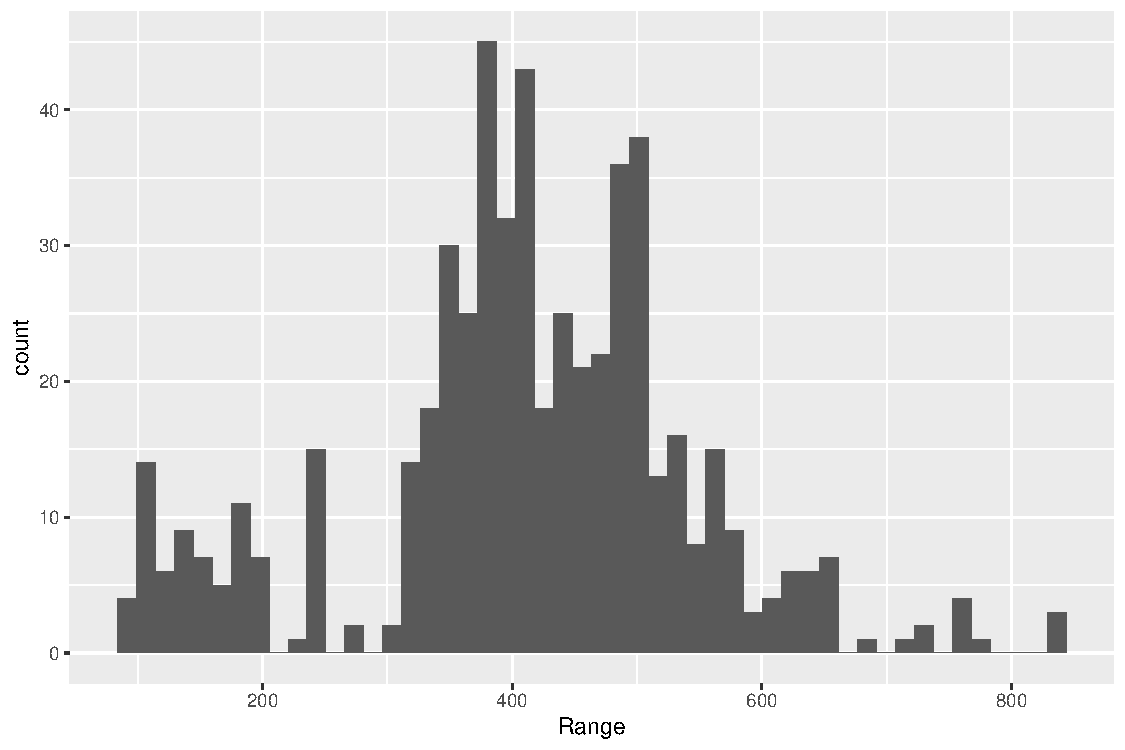
\includegraphics[width=.8\textwidth]{histogram.pdf}
\end{center}

A density plot\index{Plot!Density} using the \texttt{geom\_density()} function, is similar to a histogram in that it indicates the frequency of values. However, a density plot shows a continuous probability distribution of the data values, and as such is limited in range between 0 and 1.

The example below adds a number of elements to the basic density plot. The function \texttt{labs()} allows specification of labels for all plot elements. The \texttt{geom\_vline()} geoms add vertical lines. Note that these geoms do not receive the data from the pipe, but the data is specified using the \texttt{data} argument. The aesthetics of a vertical line map the x axis intercept to a data variable. Different line types are used for the different lines. The \texttt{annotate()} function adds text annotations to the plot. Each annotation prints a label at a set of x and y coordinates in the plot, with a specific size and horizontal justification. For example, \texttt{hjust=0} means the text is left-justified. Consult the documentation for further details. 

\begin{Rcode}
# Prepare summary statistics

mean_v <- e.clean |>
   summarize(mean_v = mean(Range), 
             median_v = median(Range), 
             lower95=quantile(Range, .025), 
             upper95=quantile(Range, .975), 
             maxdensity = max(density(Range)$y))

e.clean |>
  ggplot(aes(Range)) + 
    geom_density(kernel='gaussian', 
                 fill='lightblue') + 
    labs(x = 'Range (km)', 
         y = 'Proportion of Vehicles', 
         title='Density Plot - Electric Vehicle Range', 
         subtitle='Years 2012 to 2024', 
         caption='Lower and Upper 95 percentile, \
                  median and mean') +
    geom_vline(data=mean_v, 
               aes(xintercept=mean_v), 
               linetype='dashed') +
    geom_vline(data=mean_v, 
               aes(xintercept=median_v), 
               linetype='dotdash') +
    geom_vline(data=mean_v, 
               aes(xintercept=lower95), 
               linetype='dotted') +
    geom_vline(data=mean_v, 
               aes(xintercept=upper95), 
               linetype='dotted') + 
	annotate('text', 
	   label=paste(' L95=\n ',round(mean_v$lower95),sep=''), 
	   x = mean_v$lower95, y = mean_v$maxdensity/2, 
	   size=3.5, hjust=0) +
	annotate('text', 
	   label=paste(' Med=\n ',round(mean_v$median_v),sep=''), 
	   x = mean_v$median_v, y = mean_v$maxdensity*3/4, 
	   size=3.5, hjust=0) +
	annotate('text',
	   label=paste(' Mean=\n ',round(mean_v$mean_v),sep=''), 
	   x = mean_v$mean_v, y = mean_v$maxdensity*5/8, 
	   size=3.5, hjust=0) + 
	annotate('text',
	   label=paste(' U95=\n ',round(mean_v$upper95),sep=''), 
	   x = mean_v$upper95, y = mean_v$maxdensity/2, 
	   size=3.5, hjust=0)
\end{Rcode}

\begin{center}
  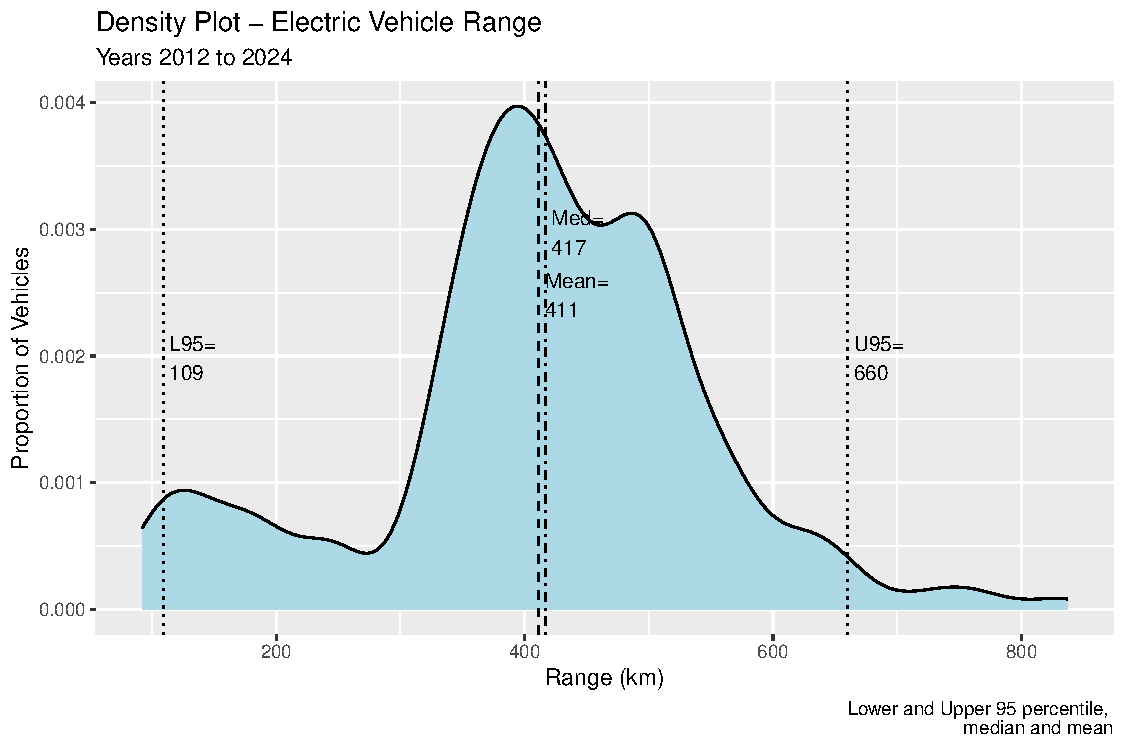
\includegraphics[width=.8\textwidth]{fuel.density.pdf}
\end{center}

The next example shows how histograms and density plots can be combined. The R code fragment below indicates only the relevant changes to the previous example.

\begin{samepage}
\begin{Rcode}
...
geom_histogram(aes(y=..density..), bins=50, 
     alpha=0.5, fill='white', color='black', ) +
geom_density(kernel='gaussian', 
     alpha=0.25, fill='lightblue') + 
...
\end{Rcode}
\end{samepage}

\begin{center}
  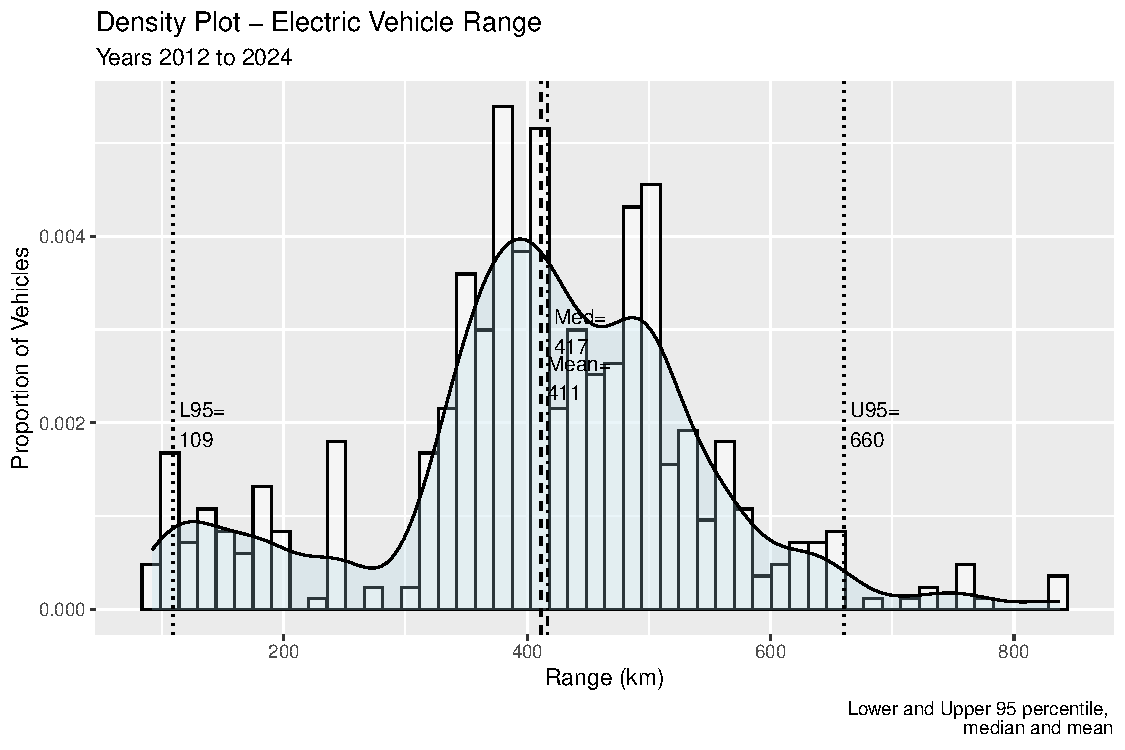
\includegraphics[width=.8\textwidth]{fuel.histogram.pdf}
\end{center}

An area plot\index{Plot!Area} is essentially a line plot where the area under the line filled. However, in contrast to a line plot, when plotting multiple data variables in an area plot, the area plot is cumulative, that is, data are stacked on top of each other. The following example first uses dplyr functions to compute a summary statistic, and then pipes the result into the \texttt{ggplot()} function. \texttt{geom\_text()} is another way to add annotations to the data. This geom uses its own aesthetic in the example below. Note that \texttt{position='jitter'} indicates that overlapping points (i.e. points with the same data values) should be randomly moved a little bit to show them separately. 

\begin{Rcode}
e.clean %>%
  group_by(Year) %>%
  summarize(meanRange = mean(Range)) %>%
  ungroup() %>%
  ggplot(aes(Year, meanRange)) + 
    geom_area(fill='purple') +
    geom_text(aes(label=round(meanRange)), 
              size=5, position='jitter') +
    labs(x='Year', y='Mean Range (km)', 
         title='Vehicle Range by Year', 
         subtitle='Years 2012-2024')
\end{Rcode}

\begin{center}
  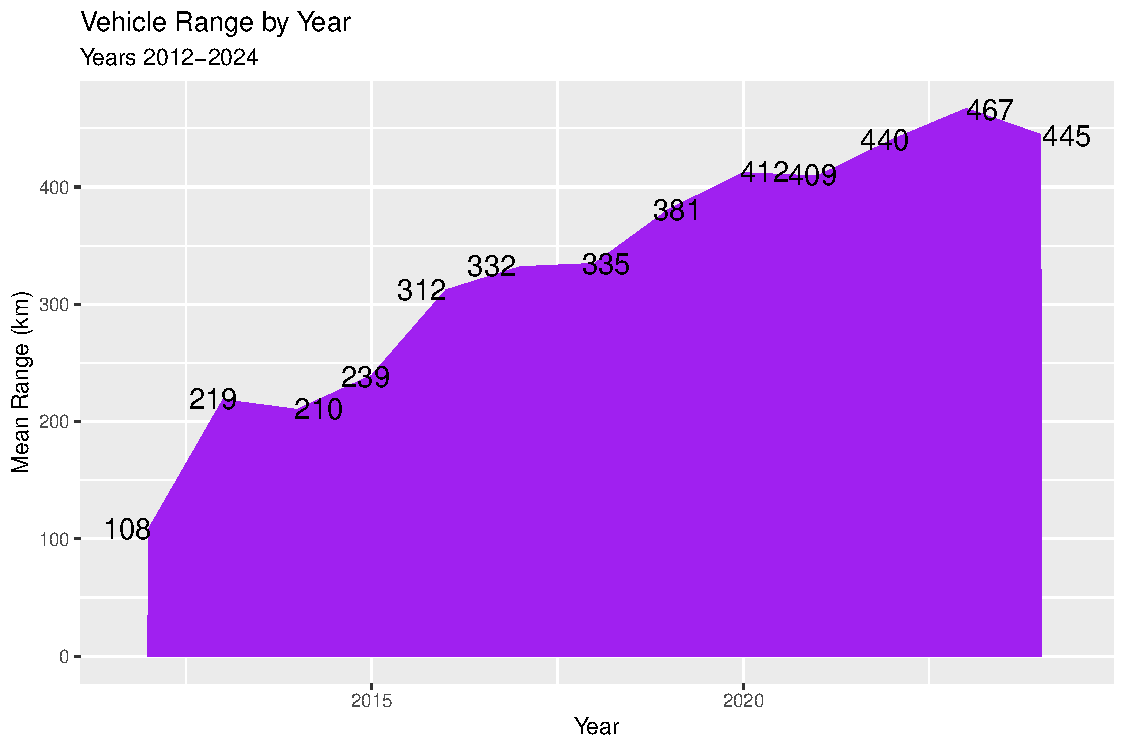
\includegraphics[width=.8\textwidth]{fuel.areaOneSeries.pdf}
\end{center}

The next example shows a column chart\index{Plot!Column chart}. Again, dplyr functions are used to create suitable summary statistics to plot, and the summarized data is then piped to \texttt{ggplot()}. The variable ''metric'' is mapped to the ''fill'' element of the plot, that is the color with which columns are filled. The \texttt{position='dodge'} argument to the the \texttt{geom\_col()} function indicates that columns are located next to each other, instead of being stacked on top of each other. 

This example also shows customization of the scales. Here, the fill scale (that is, the colour) is customized, first by specifying a colour palette, and then by providing labels for the different categories. The legend is automatically added to the right of the column plot.

\newpage
\begin{Rcode}
e.clean %>%
   group_by(Year) %>%
   summarize(meanCity = mean(City), meanHwy = mean(Hwy)) %>%
   ungroup() %>%
   pivot_longer(cols=c('meanCity', 'meanHwy'), 
                names_to='metric', 
                values_to='consumption') |>
   ggplot(aes(Year, consumption, fill=metric)) +
      geom_col(position='dodge') +
      scale_fill_brewer(palette="Paired") +
      scale_fill_discrete(labels=c("City", "Highway")) + 
      labs(x = 'Year', 
           y='Mean Fuel Consumption\n(l/100km equivalent)', 
           fill='', 
           title='Electric Vehicle Range', 
           subtitle='Years 2012 to 2024')
\end{Rcode}

\begin{center}
  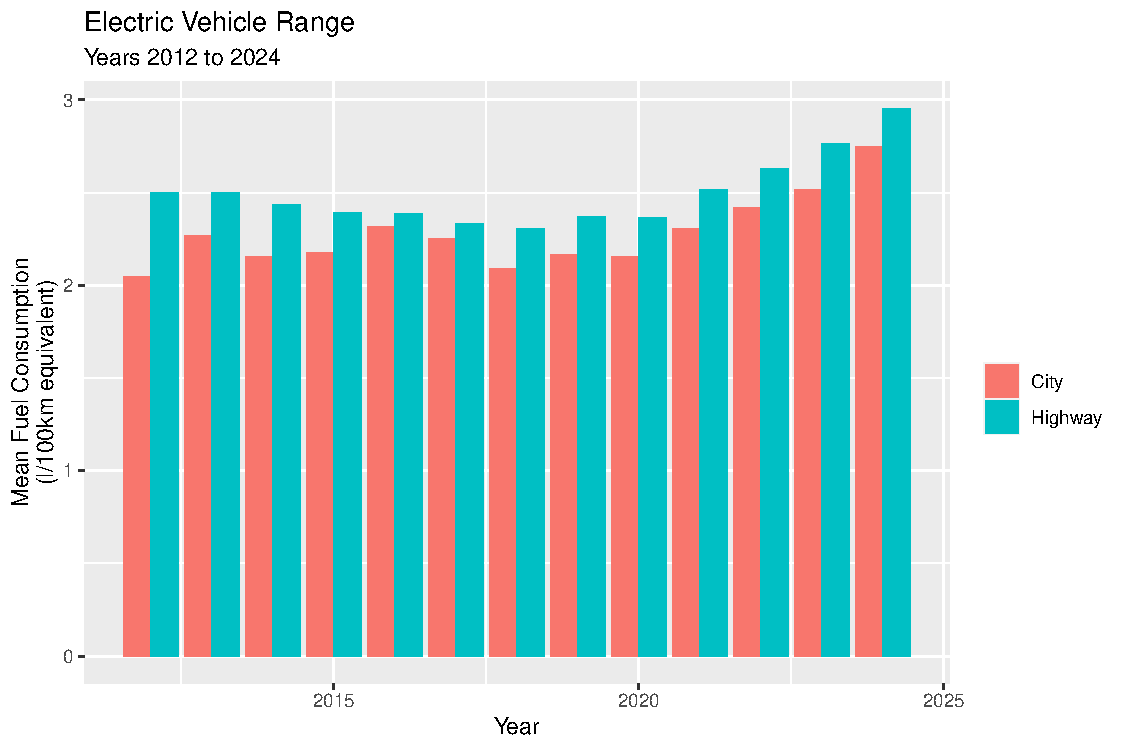
\includegraphics[width=.8\textwidth]{fuel.columns.pdf}
\end{center}

When it is clear that a plot is likely to be printed in black and white, it may be useful to omit the use of colours and instead use different fill patterns. They are provided by the \texttt{ggpattern} package that provides the \texttt{geom\_col\_pattern} geom. As shown in the code below, the aesthetics for this geom can map data values to different aspects of a fill pattern, such as the pattern type and the pattern angle.

This example also customizes the scale for the ''pattern'' geom to provide values for the different pattern types and labels for the two data series. Note that more then the required two values for patterns are listed in the example to showcase the different options provided by the \texttt{ggpattern} package. Additionally, the \texttt{guides()} function is used to omit the legend for the pattern angle (because the same data is mapped to pattern type and pattern angle) and the \texttt{theme()} function customizes the layout of the legend.

\begin{Rcode}
e.clean %>% 
   group_by(Year) %>%
   summarize(meanCity = mean(City), 
             meanHwy = mean(Hwy)) %>%
   ungroup() %>%
   pivot_longer(
        cols=c('meanCity', 'meanHwy'), 
        names_to='metric', 
        values_to='consumption') %>%
ggplot(aes(Year, consumption)) +
  geom_col_pattern(
         aes(pattern_type=metric, pattern_angle=metric),
     pattern='polygon_tiling',
     pattern_fill='white', 
     pattern_scale=0.5,
     position='dodge',
     pattern_key_scale_factor=0.4) +
  scale_pattern_type_manual(
     values = c('hexagonal', 'rhombille', 'pythagorean', 
                'truncated_square', 'rhombitrihexagonal', 
                'truncated_trihexagonal'), 
     labels=c("City", "Highway")) + 
  labs(x = 'Year', y='Mean Fuel Consumption', 
       pattern_type='', 
       title='Electric Vehicle Range', 
       subtitle='Years 2012 to 2024') +
  guides(pattern_angle=FALSE, 
         pattern_type=guide_legend(nrow=1)) + 
  theme(legend.key.size=unit(1.5, 'cm'), 
		legend.position='bottom')
\end{Rcode}

\begin{center}
  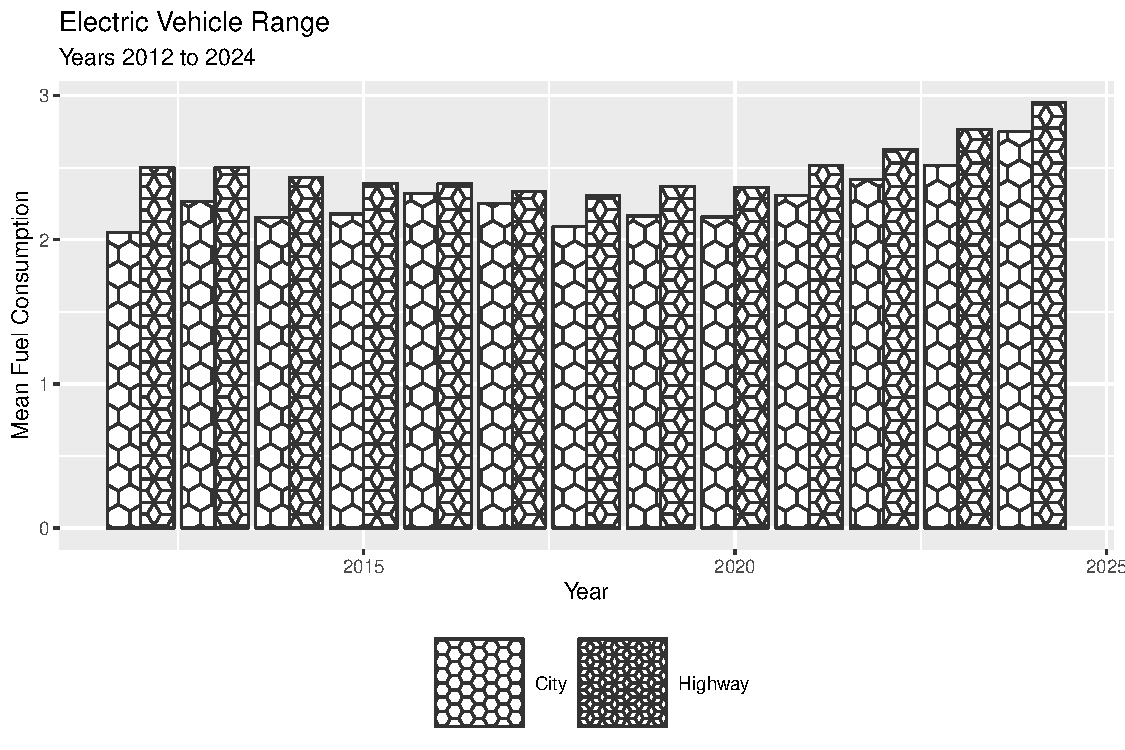
\includegraphics[width=.8\textwidth]{fuel.columnsPatterns.pdf}
\end{center}

A box plot\index{Plot!Box plot}, also known as a box-and-whisker plot\index{Plot!Box-and-whisker plot|see{Plot!Bos plot}}, is a way of displaying the distribution of data based on 5 summary statistics: the minimum, first quartile (Q1), median, third quartile (Q3), and the maximum. A box plot provides a visual summary of the spread, central tendency, and symmetry of the data. Boxplots contain the following elements:

\begin{itemize}
\item \emph{The Box:}'index{Box (in Box plot)} The bottom and top edges of the box represent the first quartile (Q1, the 25th percentile) and the third quartile (Q3, the 75th percentile), respectively. The box therefore describes the interquartile range (IQR), i.e. the distance between the first and third quartiles.
\item \emph{The Median:} Inside the box, there is usually a line that denotes the median (the 50th percentile) of the dataset. By comparing the placement of the median line to the extent of the first and third quartiles, one can judge whether the data is skewed.
\item \emph{Whiskers:}\index{Whiskers (in Box plot)} Extending from the box are lines called whiskers. One common method is to extend the whiskers to the furthest data point within 1.5 times the IQR from the quartiles. This means that the lower whisker extends to the smallest data point greater than Q1 - 1.5 * IQR and the upper whisker extends to the largest data point less than Q3 + 1.5 * IQR.
\item \emph{Outliers:}\index{Outlier (in Box plot)} Data points that fall outside of the whiskers are often considered outliers and may be plotted as individual points.
\end{itemize}

Box plots are particularly useful for displaying the distribution of data, comparing multiple distributions, and identifying outliers.

The following example introduces the \texttt{stat\_summary()} function to add a summary statistic in the form of a text label to the plot. The label is computed by the \texttt{stat(y)} function, which in turn calls \texttt{fun.y} specified within the \texttt{stat\_summary()} function itself. The function as used in this example determines how to label the outlier points in the box plot, using the \emph{text} geom and its label.

\begin{Rcode}
e.clean %>% 
  pivot_longer(cols=c('City', 'Hwy'), 
               names_to='metric', 
               values_to='consumption') %>%
ggplot(aes(x=as.factor(Year), y=consumption, fill=metric)) +
  geom_boxplot() +
  stat_summary(
    aes(label = round(stat(y), 1)),
    geom = "text", 
    size=2,
    fun.y = function(y) {
	          o<-boxplot.stats(y)$out; 
              if(length(o)==0) NA else o}) + 
  scale_fill_brewer(palette="Paired") +
  labs(x = 'Year', 
    y='Mean Fuel Consumption\n(l/100km equivalent)', 
    fill='', 
    title='Electric Vehicle Range', 
    subtitle='Years 2012 to 2024') +
  theme(legend.key.size=unit(1, 'cm'), 
        legend.position='top')
\end{Rcode}

\begin{center}
  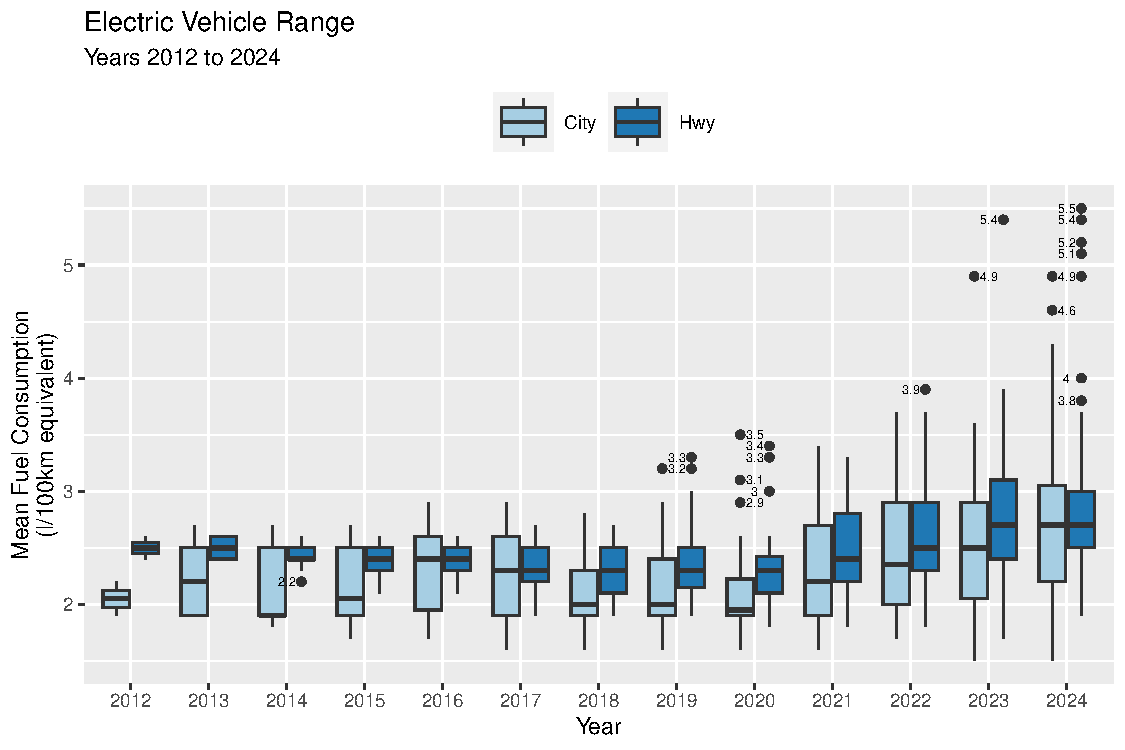
\includegraphics[width=.8\textwidth]{fuel.box.pdf}
\end{center}

Violin plots\index{Plot!Violin} are another way to visualize the spread and distribution of the data. Their width is determined by the frequency/distribution of data points. The following example introduces the \texttt{geom\_violin} geom and the \texttt{geom\_jitter} geom. As the name suggests, the jitter geom plots and ''jitters'' the data points, by moving them slightly to avoid overlap. The arguments provided to \texttt{geom\_jitter()} set the width, the color and size of the points, the fill color and the transparency level (''alpha''). the plot indicates the distribution of data, which is reinforced by the visual ''density'' of the individual data points in the plot.

\begin{samepage}
\begin{Rcode}
e.clean %>% 
  ggplot(aes(x=as.factor(Year), y=Comb)) +
    geom_violin(fill='lightblue') +
    geom_jitter(width=0.15, color='black', 
                size=1, fill=NA, alpha=0.5) + 
    scale_fill_brewer(palette="Paired") +
    labs(x = 'Year', 
         y='Mean Fuel Consumption\n(l/100km equivalent)', 
         fill='', 
         title='Electric Vehicle Range', 
         subtitle='Years 2012 to 2024')
\end{Rcode}
\end{samepage}

\begin{center}
  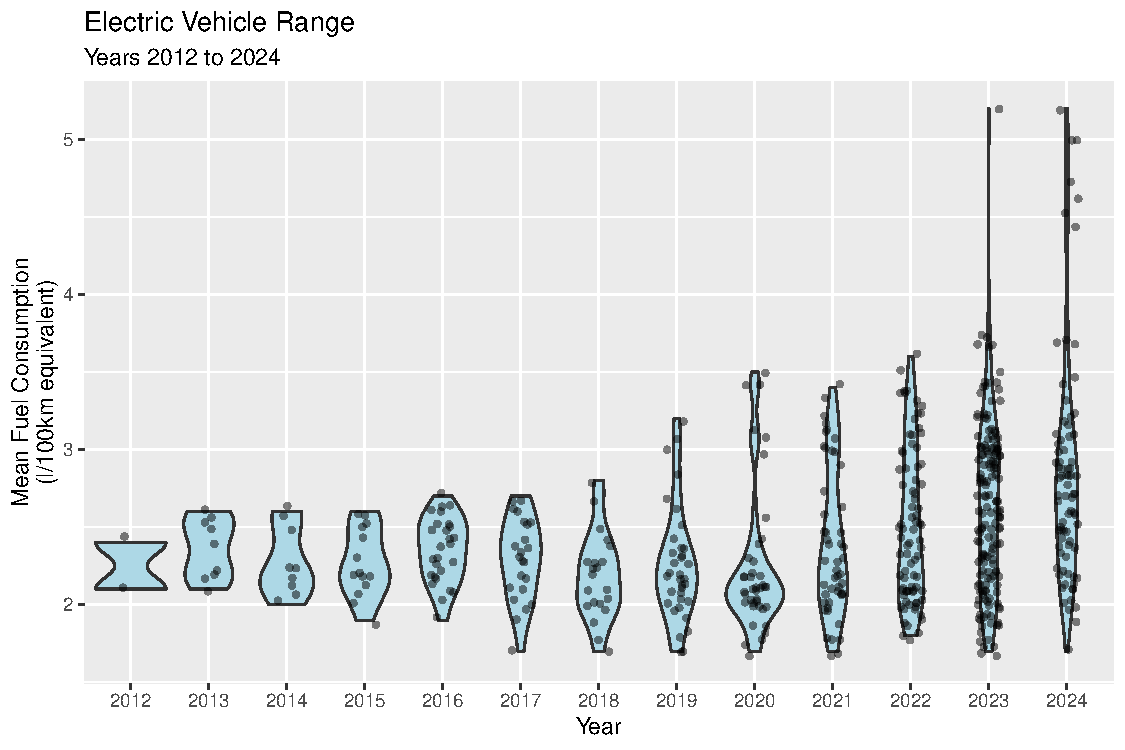
\includegraphics[width=.8\textwidth]{fuel.violin.pdf}
\end{center}

A dot plot\index{Plot!Dot} is useful for showing individual data points. In this example, the data are binned along the y axis (that is, by combined fuel economy). The stack ratio determines the horizontal separation of points.

\begin{Rcode}
e.clean %>% 
  ggplot(aes(x=as.factor(Year), y=Comb)) +
    geom_dotplot(binaxis='y', 
                 stackdir='center', 
                 stackratio=0.5,
                 binpositions='all',
                 dotsize=0.5, 
                 color='black', 
                 fill='orange') +
    scale_fill_brewer(palette="Paired") +
    labs(x = 'Year', 
         y='Mean Fuel Consumption\n(l/100km equiv)', 
         fill='', 
         title='Electric Vehicle Range', 
         subtitle='Years 2012 to 2024')
\end{Rcode}

\begin{center}
  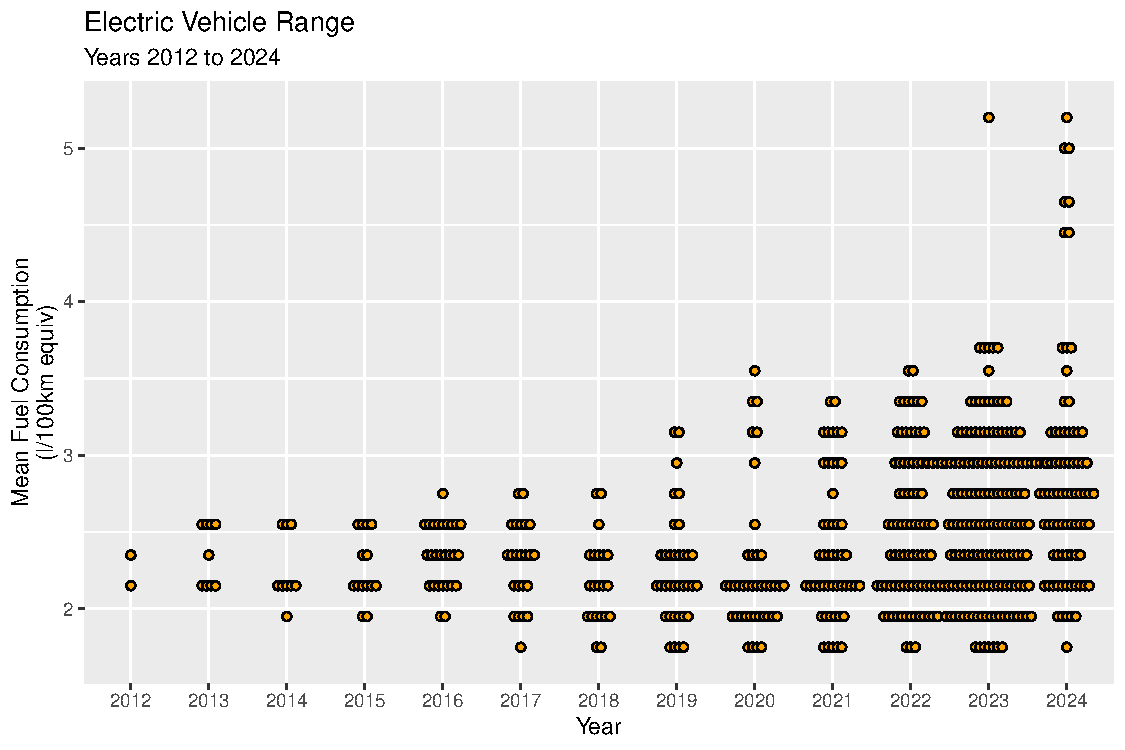
\includegraphics[width=.8\textwidth]{fuel.dotplot.pdf}
\end{center}

Instead of using a jitter plot with a violin plot, it is sometimes better to combine a violin plot with a dot plot, as in the following example.

\begin{samepage}
\begin{Rcode}
e.clean %>% 
  filter(Year > 2019) %>%
  ggplot(aes(x=as.factor(Year), y=Comb)) +
    geom_dotplot(binaxis='y', 
                 stackdir='center', stackratio=0.5,
                 binpositions='all', dotsize=0.5, 
                 color='black', fill='orange') +
    geom_violin(color='black', fill=NA) + 
    stat_summary(fun.data=mean_sdl, 
                 fun.args=list(mult=1), 
                 size=1, color='blue', 
                 geom="pointrange") +
    scale_fill_brewer(palette="Paired") +
    labs(x = 'Year', 
         y='Mean Fuel Consumption\n(l/100km equiv)', 
         fill='', 
         title='Electric Vehicle Range', 
         subtitle='Years 2020 to 2024') +
     theme(legend.position='none')
\end{Rcode}
\end{samepage}

\begin{center}
  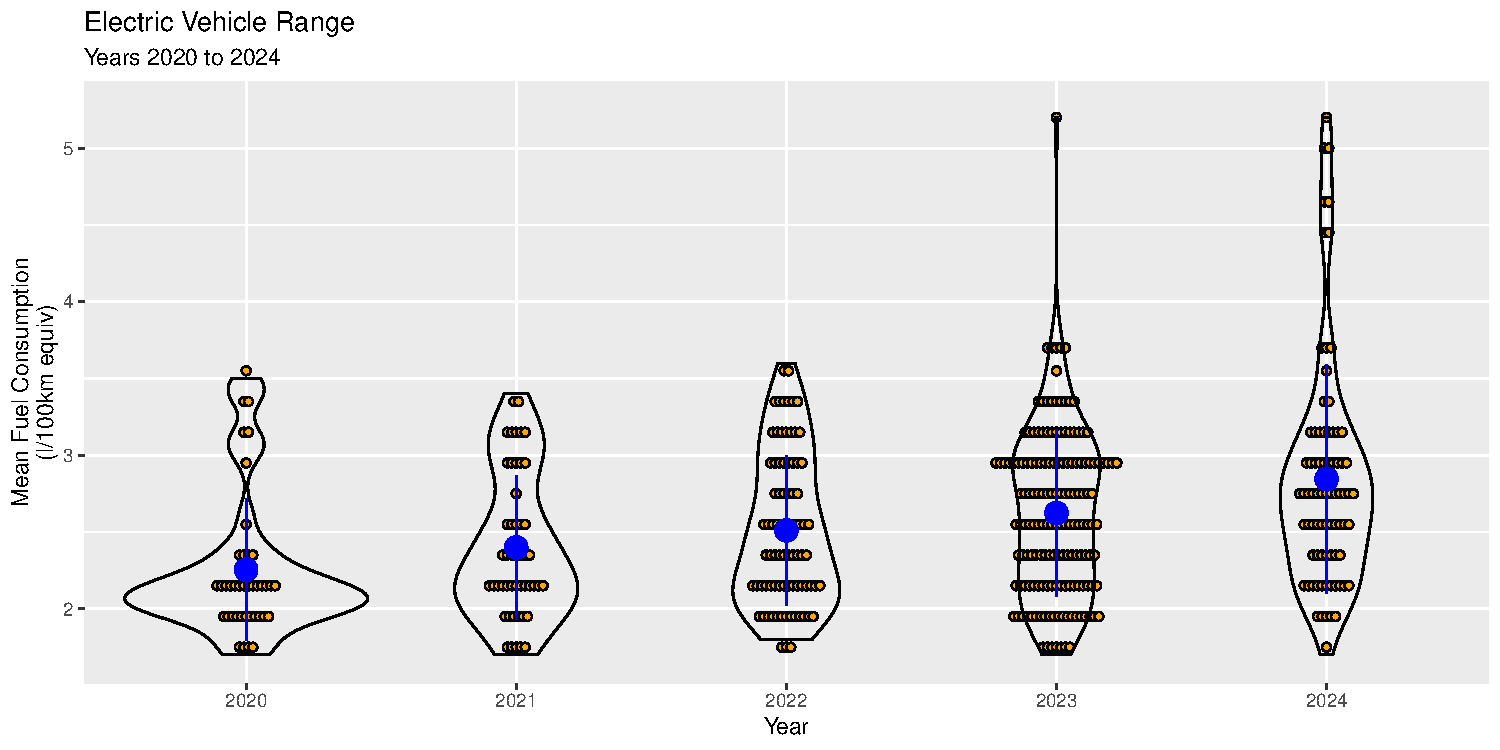
\includegraphics[width=.8\textwidth]{fuel.dotplotjviolinsummary.pdf}
\end{center}

A count plot\index{Plot!Count} is useful to show the count of data values as the size of a point. In the following example, the point size is determined by the count of values in each combination of ''Year'' and ''Category''. All points have the same color, and the area is scaled to a maximum size of 10 using 6 different sizes. Additionally, this examples shows further customization of the plot legend using the \texttt{theme()} function, by surrounding the legend with a black rectangle without fill (transparent). The \texttt{guides()} function omits a legend for the color. 

\begin{samepage}
\begin{Rcode}
e.clean %>% 
  ggplot(aes(as.factor(Year), as.factor(Category))) +
    geom_count(color='darkolivegreen4')+
    scale_size_area(max_size=10, n.breaks=6) + 
    scale_color_brewer(palette="Paired") +
    scale_y_discrete(
      labels=c('Compact', 'Large', 'Mid-Size', 'Pickup truck', 
               'Subcompact', 'Two-seater', 'SUV (standard)', 
               'SUV (small)', 'Station Wagon (small)')) + 
    guides(color=FALSE) +
    labs(x = 'Year',
         y='Category', 
         fill='', 
         title='Electric Vehicle Models by Category', 
         subtitle='Years 2012 to 2024') +
    theme(legend.background=element_blank(), 
          legend.box.background=element_rect(color='black',fill=NA),
          legend.key.size=unit(1, 'cm'))
\end{Rcode}
\end{samepage}

\begin{center}
  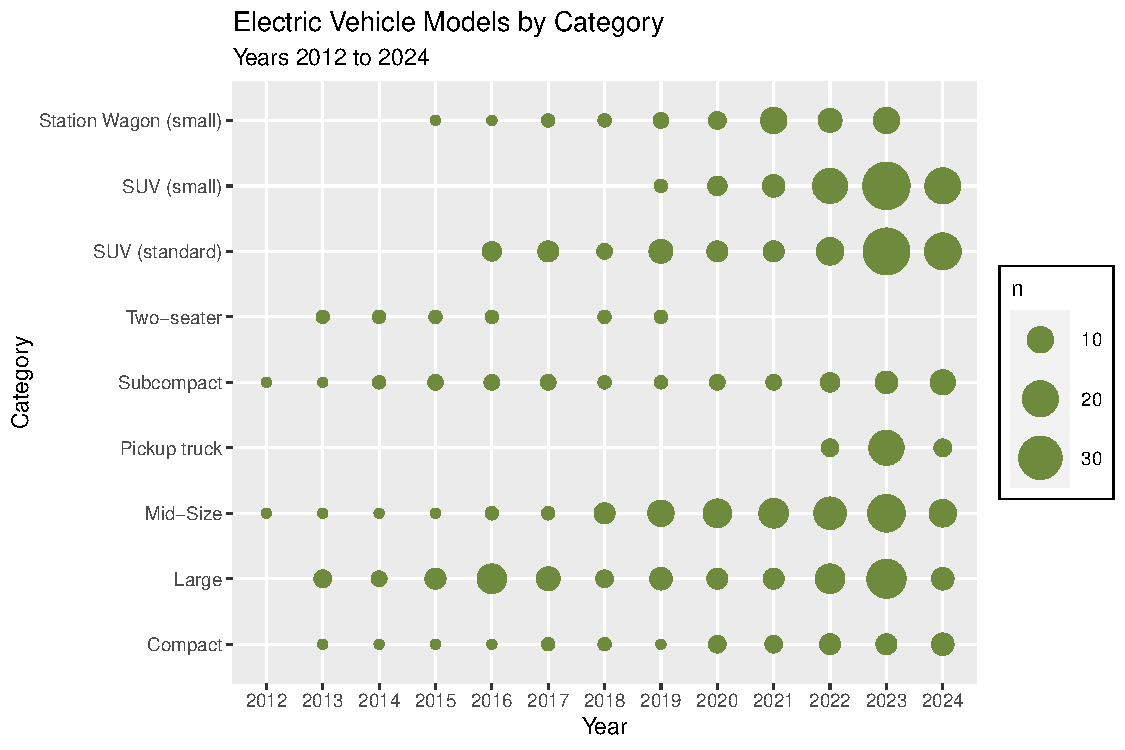
\includegraphics[width=.8\textwidth]{fuel.count.pdf}
\end{center}

A similar effect can be achieved with jitter plot, where the size of the points ''cloud'' indicates is used analogous to the size of the point. Visually, the following plot achieves a similar goal as the previous dot plot. Here, the same variable is mapped to both the x axis as well as the color element, but the \texttt{guides} function omits a legend for the colour element.

\begin{samepage}
\begin{Rcode}
e.clean %>% 
  ggplot(aes(x=as.factor(Year), 
             y=as.factor(Category), 
             color=as.factor(Year))) +
    geom_jitter(width=0.2, height=0.2) +
    scale_color_manual(values=c25) +
    scale_y_discrete(
      labels=c('Compact', 'Large', 'Mid-Size', 
               'Pickup truck', 'Subcompact',
               'Two-seater', 'SUV (std)', 
               'SUV (sm)', 'Station Wagon (sm)')) + 
    guides(color=FALSE) +
    labs(x = 'Year', 
         y='Category', 
         fill='Make', 
         title='Electric Vehicle Models by Category', 
         subtitle='Years 2012 to 2024')
\end{Rcode}
\end{samepage}

\begin{center}
  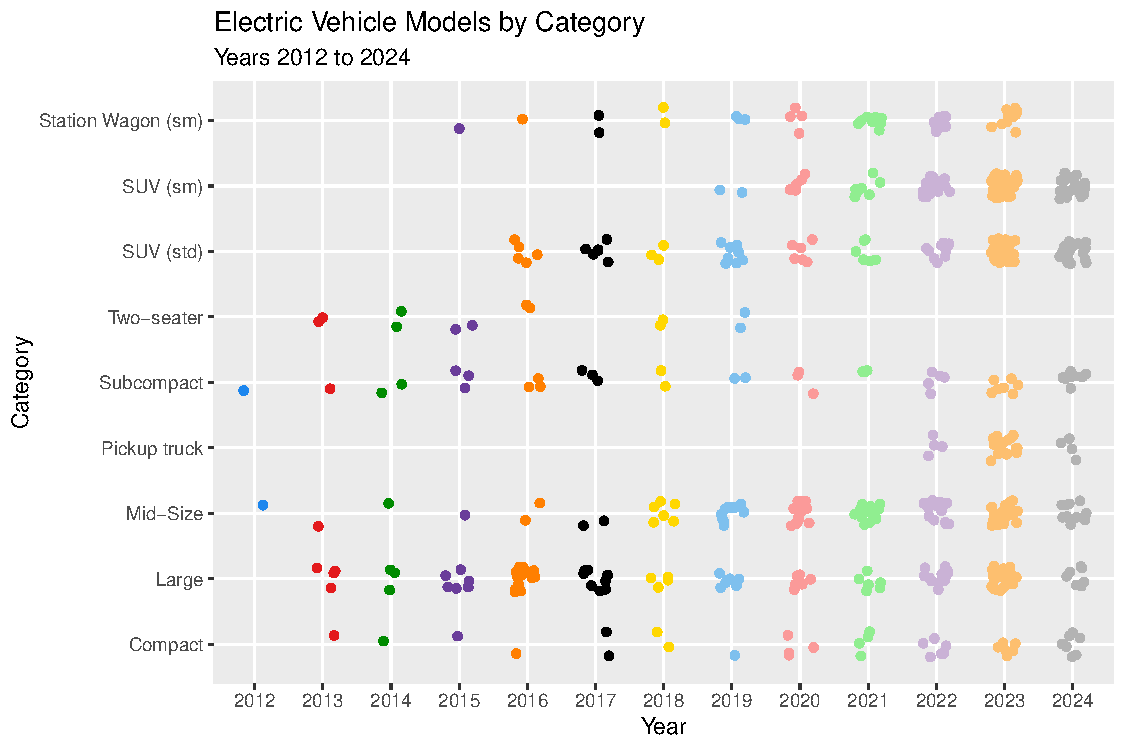
\includegraphics[width=.8\textwidth]{fuel.jitterdiscrete.pdf}
\end{center}

A points plot\index{Plot!Points|see{Plot!Bubble chart}}, sometimes called a bubble chart\index{Plot!Bubble chart}, generalizes the count plot. Whereas the count plot uses the number of data values to determine the size of the point, the points plot allows one to provide an explicit mapping for the point size. However, the following example also maps the size of the point to the count of values by ''Year'' and ''Category'', while the colour is mapped to the ''Category'' variable. 

The point size scale is continuous in the range from 0 to 20, the color scale is set to the ''tron'' colour palette, while the y axis is continuous. The colous are mapped to specific labels for displaying in the legend. Note that the legend contains information both for the size as well as the colour of the points.

\begin{samepage}
\begin{Rcode}
e.clean %>% 
  group_by(Year, Category) %>%
  summarize(totalcount=n(), meanRange=mean(Range)) %>%
  ungroup () %>%
ggplot(aes(x=as.factor(Year), y=meanRange, 
           size=totalcount, color=Category)) +
  geom_point(alpha=0.8) +
  scale_size_continuous(range=c(0, 20)) +
  scale_color_tron() + 
  scale_y_continuous(labels=scales::comma) + 
  scale_color_discrete(
     labels=c('Compact', 'Large', 'Mid-Size', 'Pickup truck', 
              'Subcompact', 'Two-seater', 'SUV (dtd)', 
              'SUV (sm)', 'Station Wagon (sm)')) + 
  labs(x = 'Year', y='Range', 
       fill='Make', size='Number of Models', 
       title='Electric Vehicles by Year and Category', 
       subtitle='Years 2012 to 2024', ) +
  guides(color=guide_legend(position='right'), 
         size=guide_legend(position='right')) +
  theme(legend.background=element_blank(), 
        legend.box.background=element_rect(color='black', fill=NA),
        legend.key.size=unit(1, 'cm')) 
\end{Rcode}
\end{samepage}

\begin{center}
  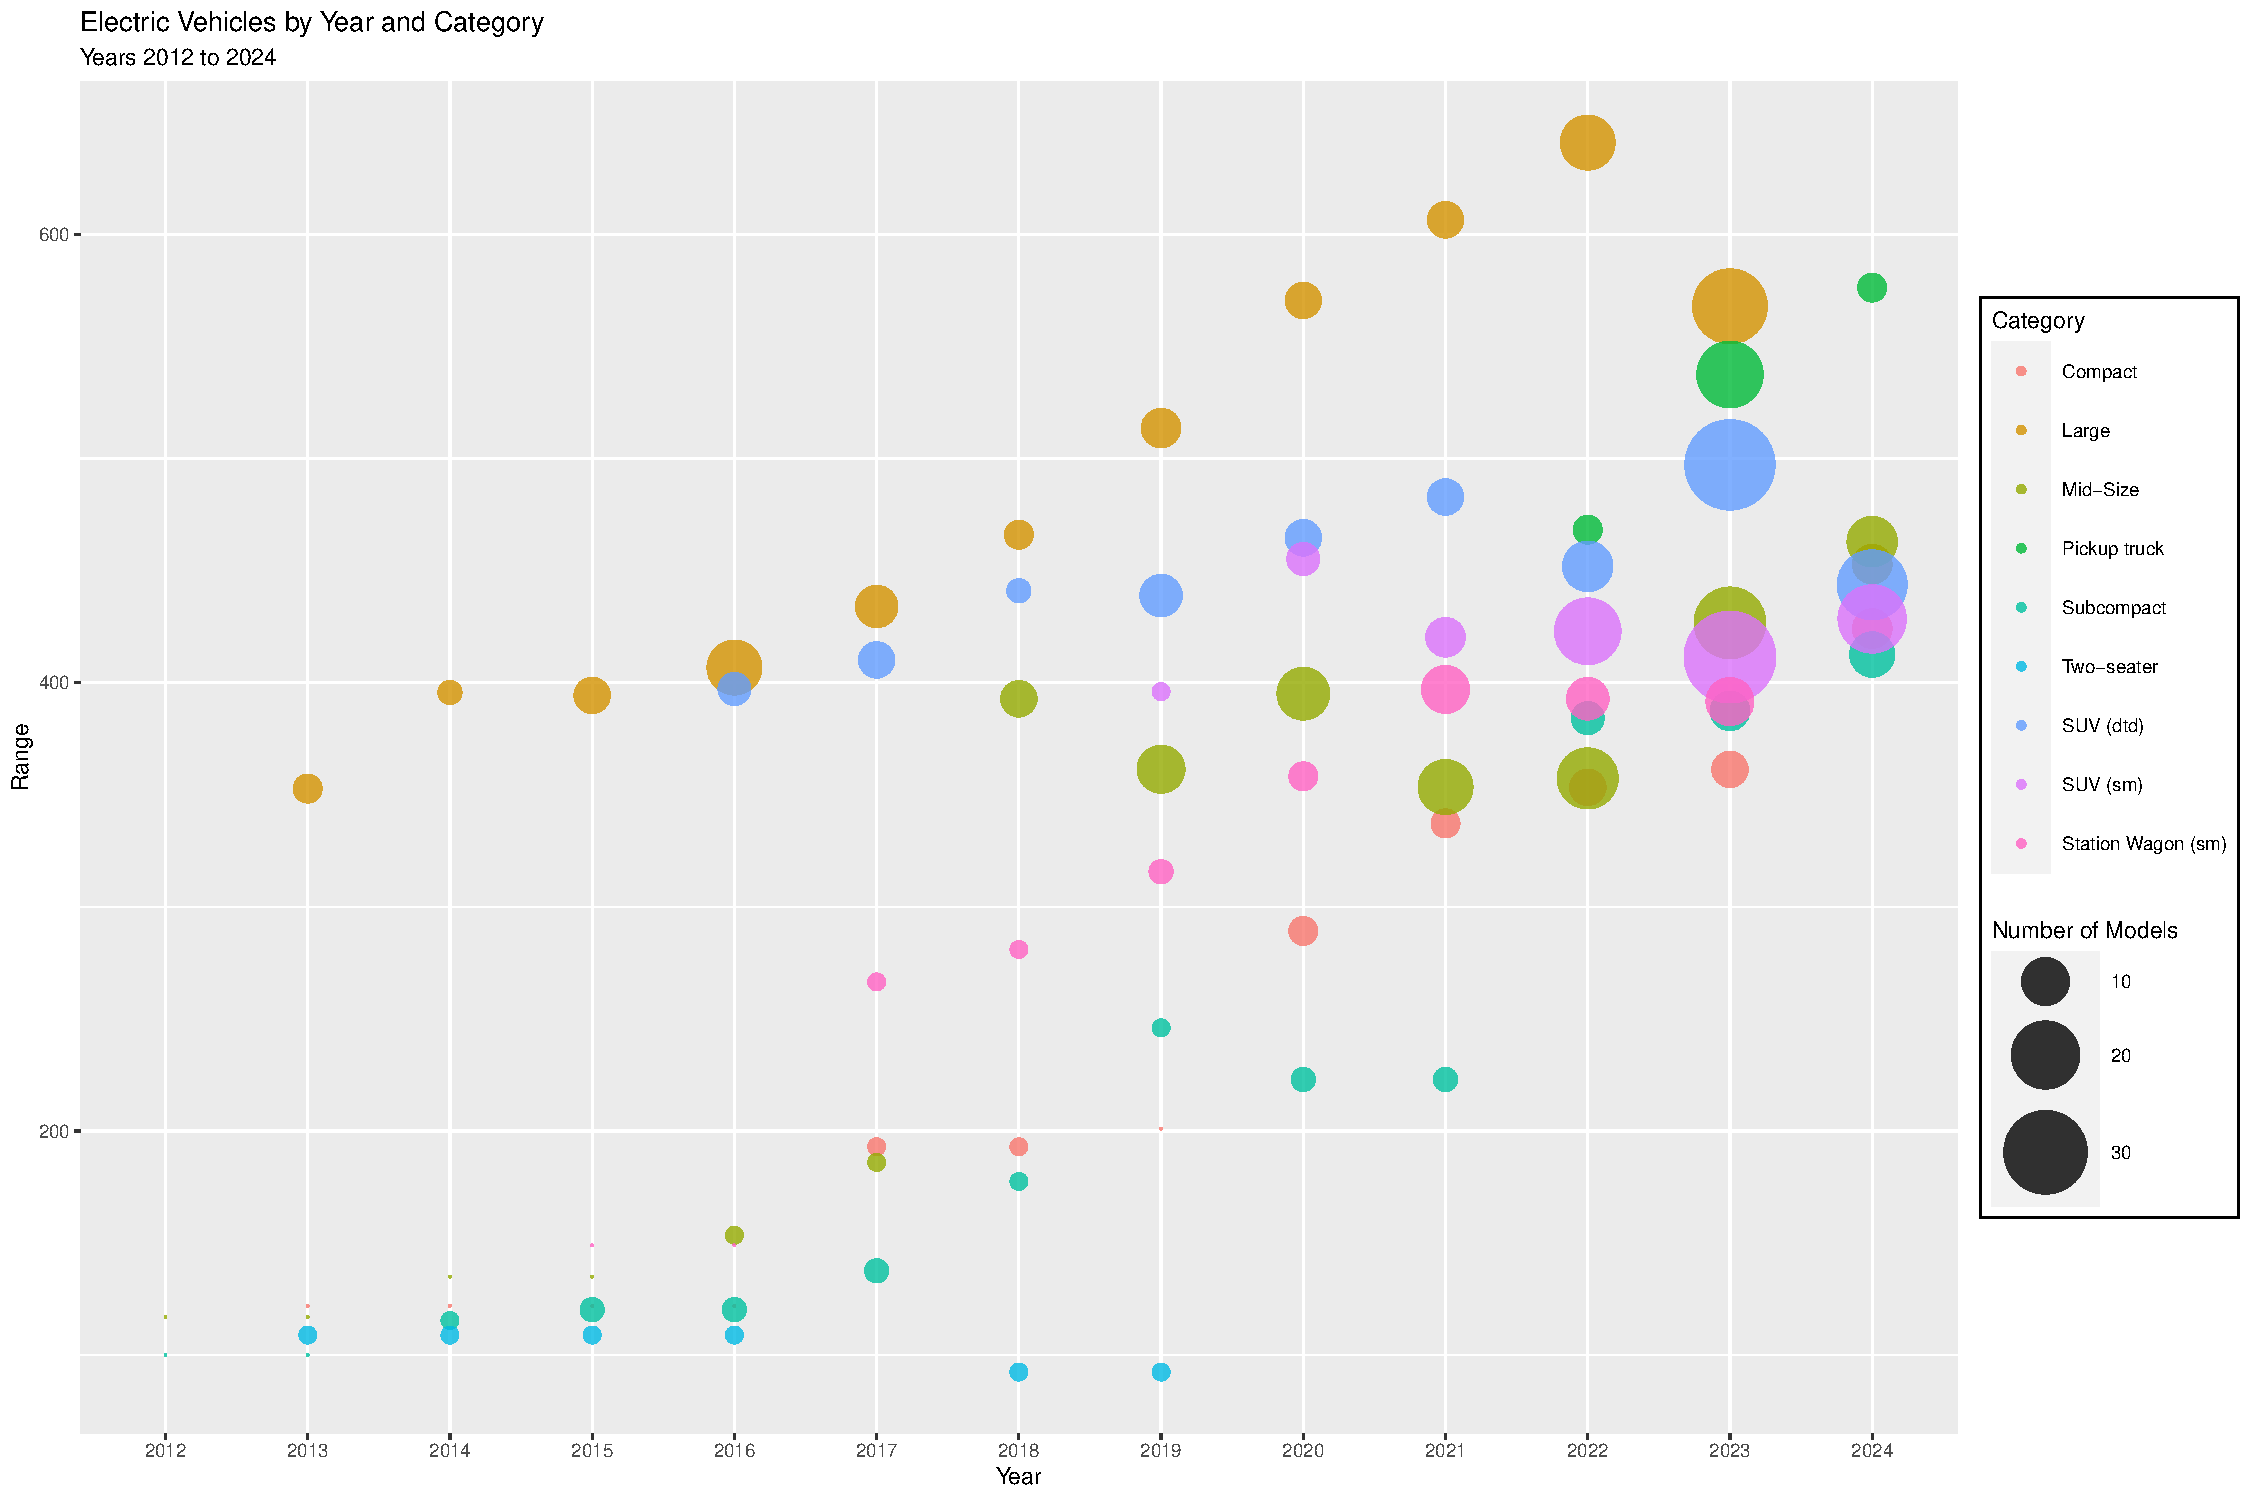
\includegraphics[width=.8\textwidth]{fuel.pointsSize.pdf}
\end{center}

The next example uses two geoms, \texttt{geom\_line()} to show a line plot\index{Plot!Line} and \texttt{geom\_point()} to also include the data points themselves. While visually not very informative in this case, the example illustrates an aesthetic that maps variables to five different plot elements. However, the same variable ''Category'' is here mapped to three different plot elements, the colour (of both points and lines), the shape of a point, and the style or type of the line. The code R fragment below omits specification of labels and theme information for the legend, which may be assumed similar to the above example.  

\begin{samepage}
\begin{Rcode}
e.clean %>% 
  filter(Year >= 2022 & Year <= 2023) %>%
  filter(Comb <= 4) %>%
  filter(Category != 'PL') %>%
  filter(Category != 'T') %>%
ggplot(aes(Comb, Range, 
           color=Category, 
           shape=Category, 
           linetype=Category)) +
  geom_line(size=1) + 
  geom_point(size=4) + 
  scale_color_manual(values=c25, 
    labels=c('Compact', 'Large', 'Mid-Size', 
             'Subcompact', 'SUV (std)', 
             'SUV (sn)', 'Station Wagon (sm)')) + 
  scale_linetype(
    labels=c('Compact', 'Large', 'Mid-Size', 
             'Subcompact', 'SUV (std)', 
             'SUV (sm)', 'Station Wagon (sm)')) + 
  scale_shape(
    labels=c('Compact', 'Large', 'Mid-Size', 
             'Subcompact', 'SUV (std)', 
             'SUV (small)', 'Station Wagon (sm)')) + 
...
\end{Rcode}
\end{samepage}

\begin{center}
  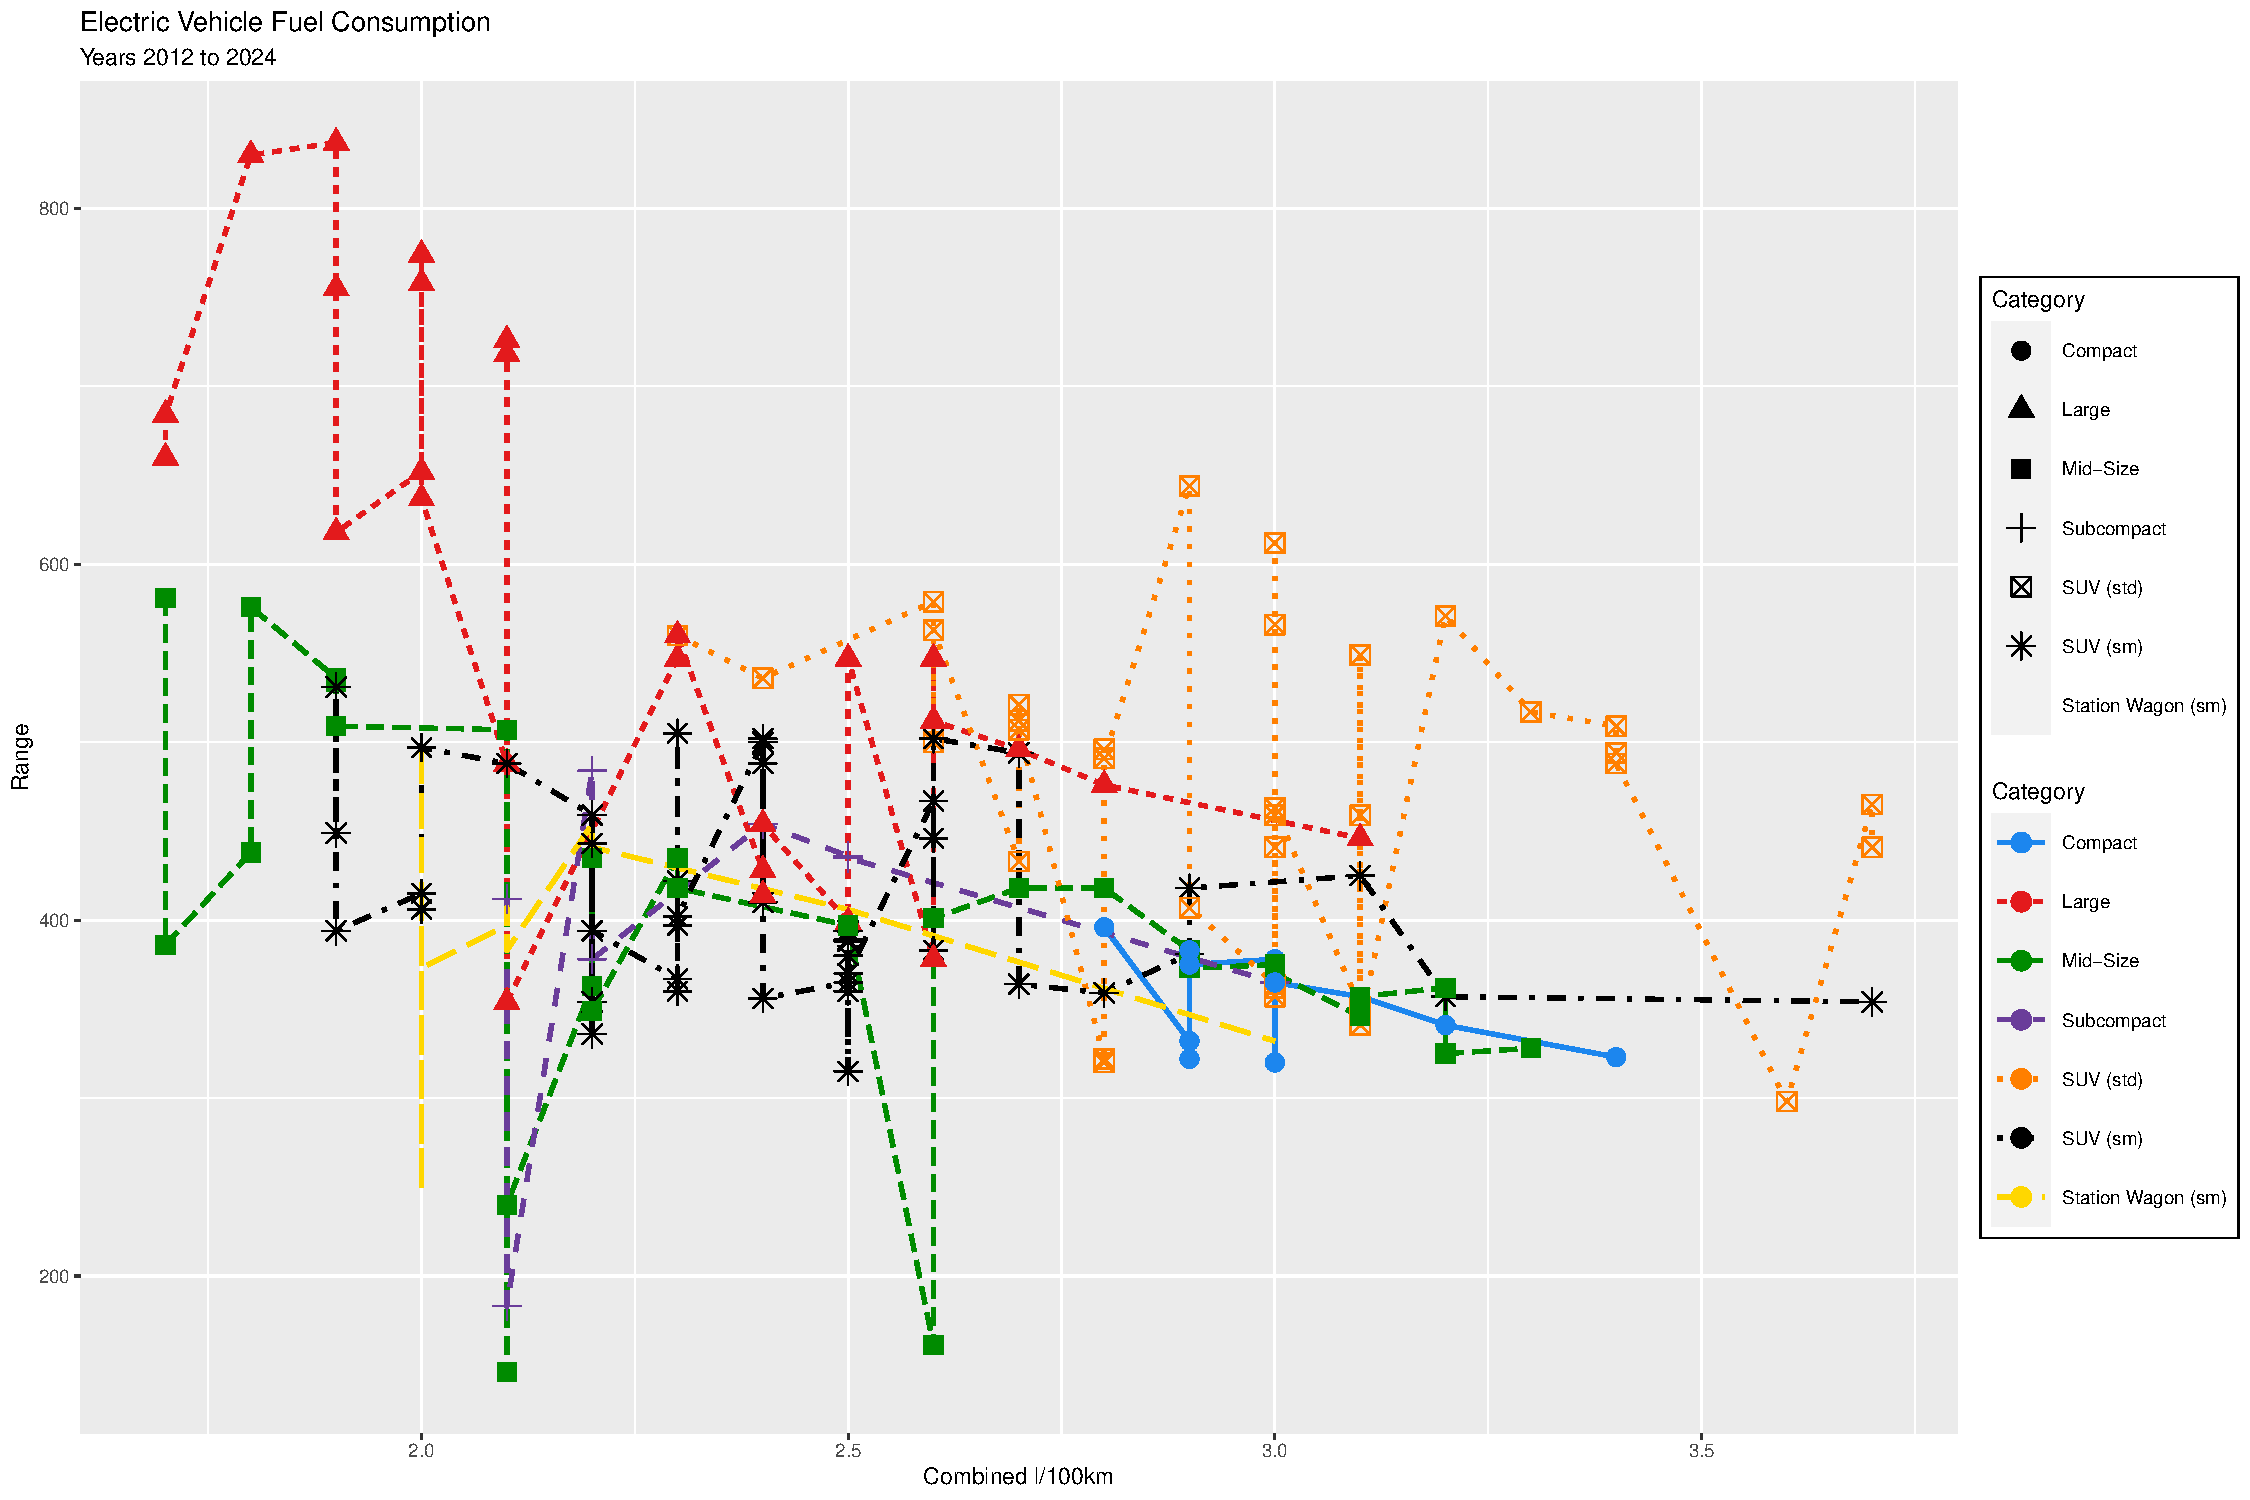
\includegraphics[width=.8\textwidth]{fuel.linesPoints.pdf}
\end{center}

To add ''steps'' to the line, one can use the \texttt{geom\_step()} instead of \texttt{geom\_line()}, as in the following example.

\begin{samepage}
\begin{Rcode}
...
     geom_step(size=1) + 
... 
\end{Rcode}
\end{samepage}

\begin{center}
  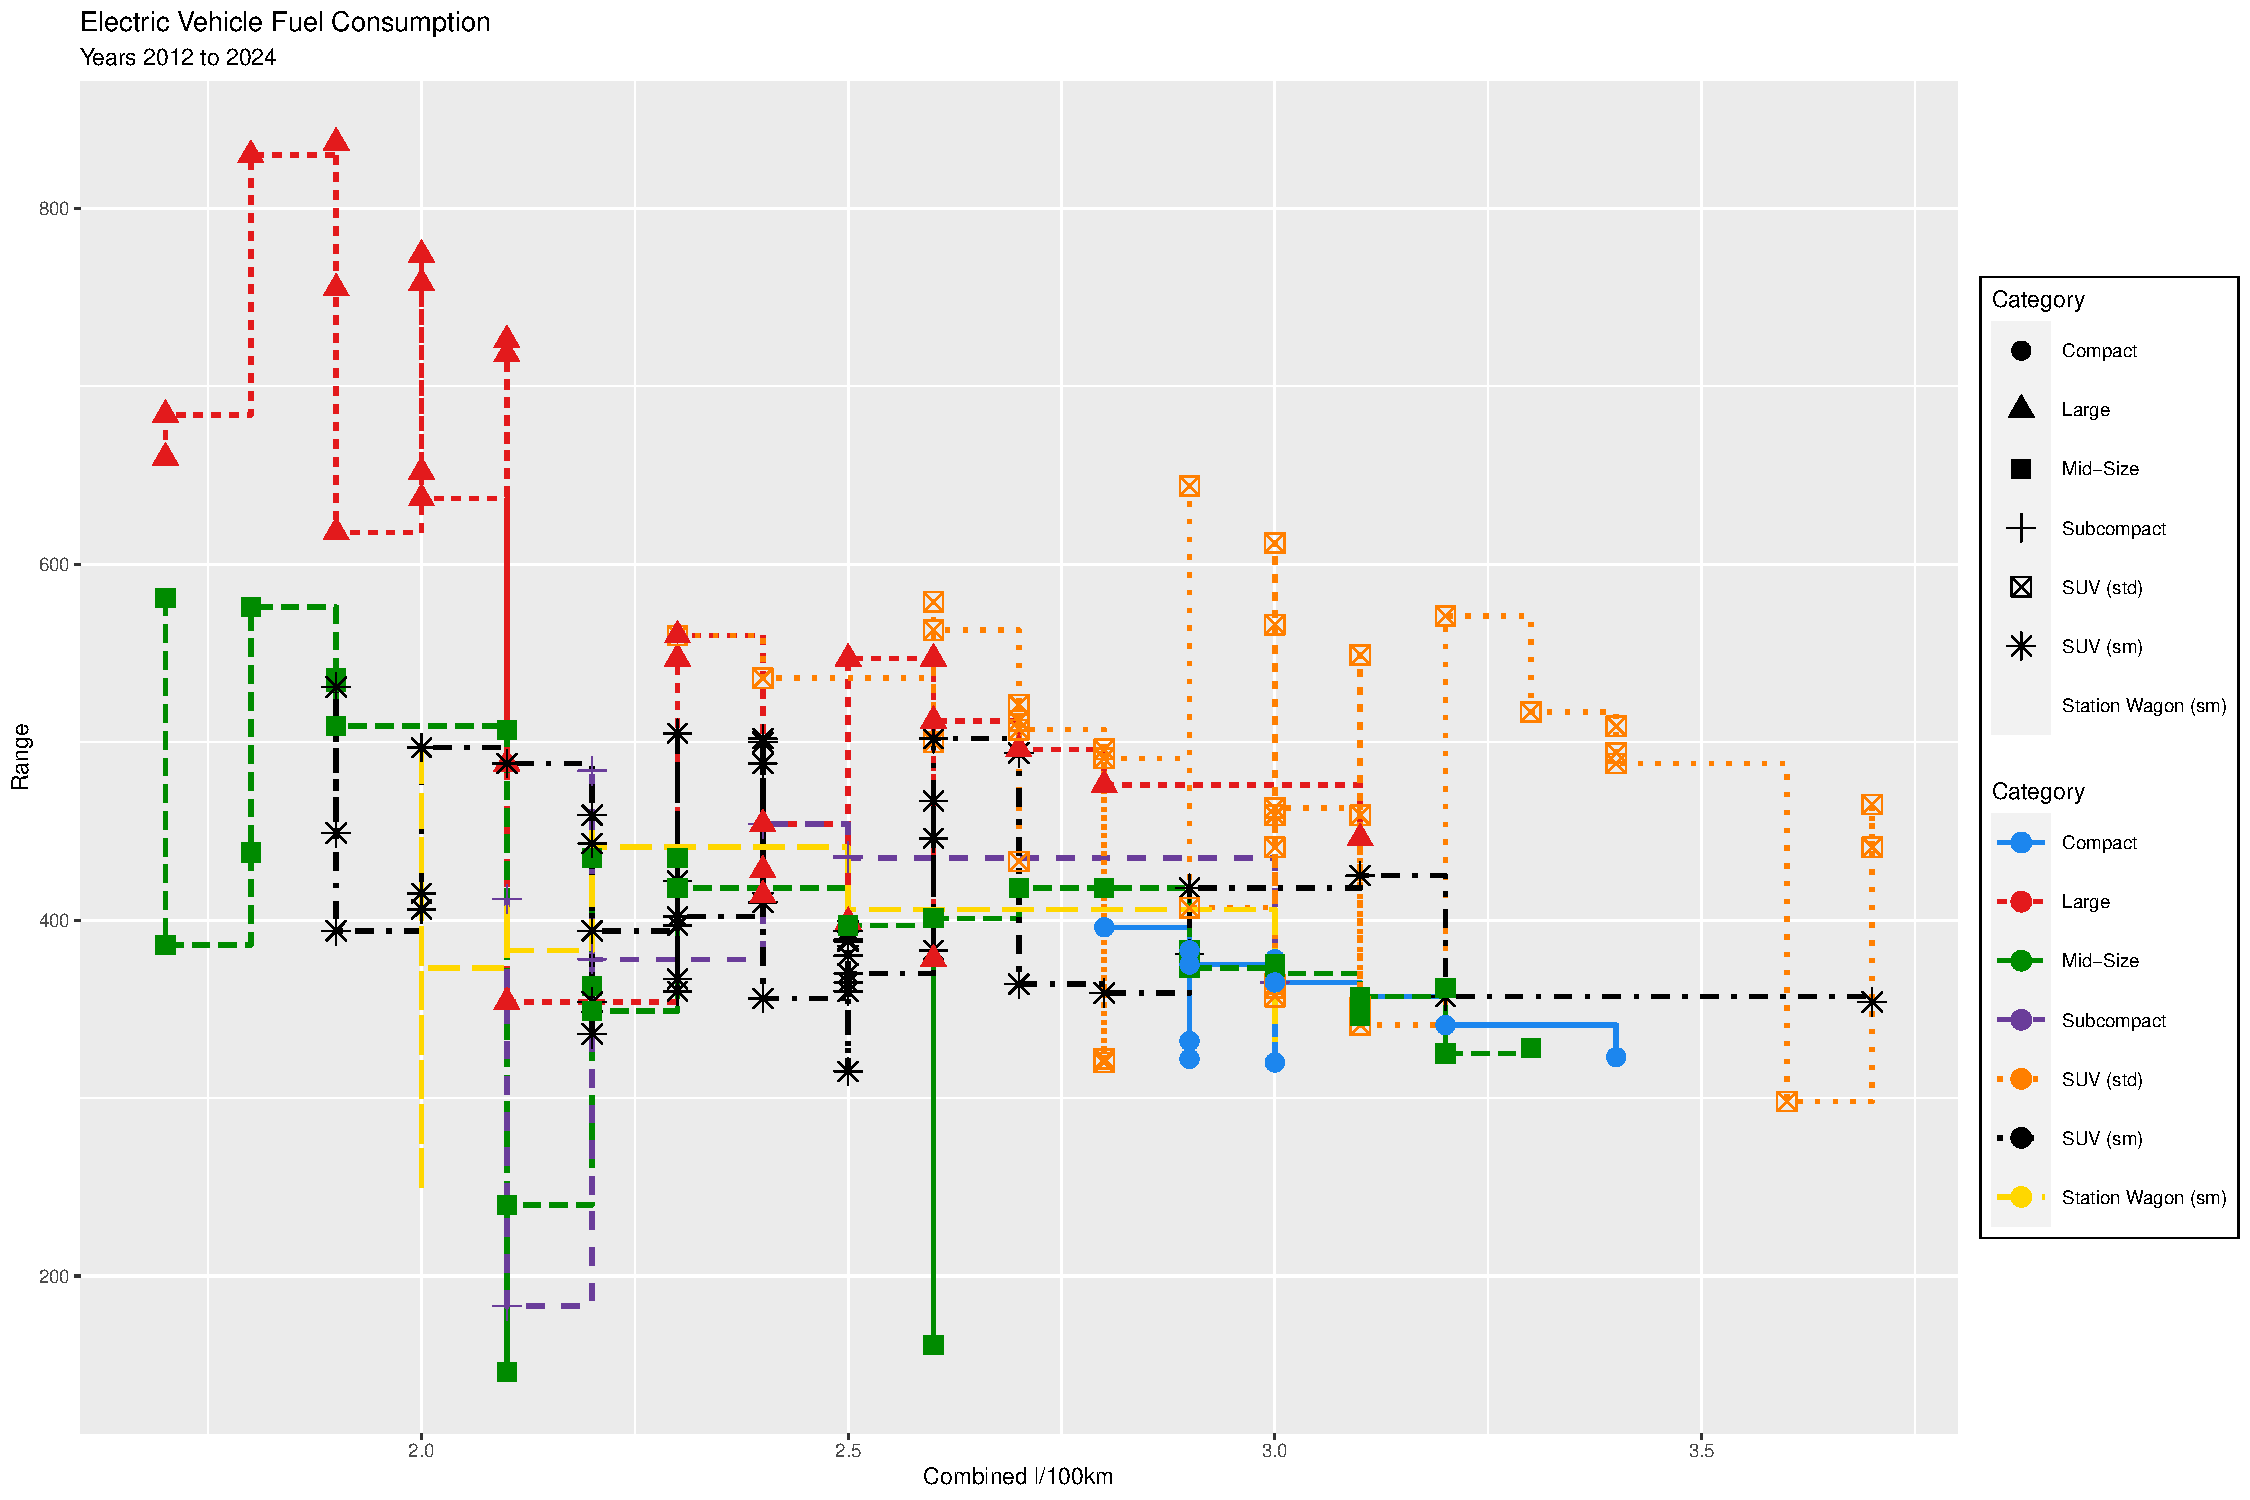
\includegraphics[width=.8\textwidth]{fuel.steps.pdf}
\end{center}

A pie chart\index{Plot!Pie chart} is produced in ggplot2 by taking a stacked bar chart, and ''bending'' it by plotting on a polar coordinate system. The following example uses the \texttt{coord\_polar()} function to specify a coordinate system where the ''y'' axis is mapped to the angle of rotation, \texttt{direction=-1} indicates clock-wise rotation and \texttt{start=0} indicates to begin the chart at the top of the ''pie''. The \texttt{geom\_text()} geom is used to specify labels and compute their position in the pie chart. It provides its own aesthetic for the label's color and position. Note that it assumes a stacked bar chart so that \texttt{position\_stack(vjust=0.5)} positions the label vertically in the center of the area. When plotted in the polar coordinate system, this translates to the label centered in the pie slice. 

\begin{samepage}
\begin{Rcode}
e.clean %>% 
  filter(Year==2023) %>%
  group_by(Make) %>% summarize(totalcount = n()) %>%
  filter(totalcount >= 5) %>%
  ungroup() %>%
ggplot(aes(x='', y=totalcount, fill=Make)) +
  geom_bar(stat='identity', 
           color='black', size=0.25, width=1) + 
  coord_polar('y', direction=-1, start=0) +
  geom_text(aes(
     label=ifelse(totalcount >= 5,totalcount,'')), 
     color='lightgrey', 
     position = position_stack(vjust=0.5)) +
  scale_y_continuous(labels=NULL) + 
  scale_color_brewer(palette="Paired") +
  labs(x = '', y = '',  fill='Make', 
       title='Electric Vehicle Offerings by Make', 
       subtitle='2023, Makes with >= 5 models') +
  theme_void() +
  theme(legend.key.size=unit(1, 'cm'))
\end{Rcode}
\end{samepage}

\begin{center}
  \includegraphics[width=.5\textwidth]{fuel.pie.pdf}
\end{center}

A donut chart\index{Plot!Donut chart} is simply a pie chart with a hole in the center. As the pie chart in ggplot2 is a ''bent'' bar chart, the hole is achieved by adding ''whitespace'' to the right of the stacked bars (that is, by moving the x axis limits), which will end up getting ''bent'' into the hole in the center (recall that the \texttt{coord\_polar()} function bends clock-wise).

\begin{samepage}
\begin{Rcode}
holesize <- 2

....

 ggplot(aes(x=holesize, y=totalcount, fill=Make)) +
   geom_col() + 
   xlim(c(0.2, holesize+0.5)) +
     
...

\end{Rcode}
\end{samepage}

\begin{center}
  \includegraphics[width=.5\textwidth]{fuel.donut.pdf}
\end{center}

A radar plot\index{Plot!Radar}, sometimes called a spiderweb plot, is useful to show a comparison of different objects on a range of variables. In R, the radar plot is produced by its own library, \texttt{ggradar}. In contrast to \texttt{ggplot}, \texttt{ggradar} requires its data in ''wide'' format, that is, rather than a single column that provides values for different categories, the values for each category must be provided in their own column. 

The following example computes some summary statistics, and scales the resulting variables to a range between 0 and 1, i.e. it standardizes them using the \texttt{mutate\_at()} function. The radar plot does not require an aesthetic specification, as it is based on the number of columns in the data frame or tibble provided from the pipe.

\begin{samepage}
\begin{Rcode}
e.clean %>% 
  filter(Year == 2023) %>% group_by(Make) %>%
  summarize(meanCity = 1/mean(City), 
            meanHwy = 1/mean(Hwy), 
            meanRange = mean(Range)/100, 
            nModels = n()) %>%
  filter(nModels >= 5) %>% ungroup() %>%
  select(-nModels) %>%
  mutate_at(vars(-Make), rescale) %>%
  ggradar(axis.labels=
             c('City', 'Highway', 'Range (100km)'), 
          values.radar='', 
          group.line.width=0.75, 
          group.point.size=3) +
  scale_color_ucscgb() +
  labs(x = '', y = '',  fill='Make', 
       title='Canadian Fuel Consumption Data', 
       subtitle='2023, Makes with more than 5 models')
\end{Rcode}
\end{samepage}

\begin{center}
  \includegraphics[width=.75\textwidth]{fuel.radar.pdf}
\end{center}

Sometimes, it is useful to compare trends of variables that use different scales. However, beware of the potential for misuse; that is, it is easy to visually suggest correlations where none exist. The following example includes three line plots (\texttt{geom\_line()}) and specifies a secondary y axis\index{Secondary axis}\index{Axis!secondary|see{Secondary axis}} using \texttt{sec.axis=sec\_axis(\ldots)}. In ggplot2, the secondary axis cannot be arbitrary but must be a scaled version of the primary axis. In this example, it is scaled by multiplying by one hundred using the formulat \texttt{~ .*100}. Accordingly the data is provided by dividing by a hundred using \texttt{mutate()}.

\begin{Rcode}
e.clean %>% 
   group_by(Year) %>%
   summarize(meanCity = mean(City), 
             meanHwy = mean(Hwy), 
             meanRange = mean(Range)) %>%
   ungroup() %>%
   mutate(meanRange2 = meanRange/100) %>%
ggplot(aes(x=Year)) +
  scale_color_manual(name='Region', 
     values=c('Mean City' = 'red', 
              'Mean Highway' = 'blue', 
              'Mean Range' = 'orange')) +
  geom_line(aes(y=meanCity, color='Mean City')) + 
  geom_line(aes(y=meanHwy, color='Mean Highway')) +
  geom_line(aes(y=meanRange2, color='Mean Range')) +
  scale_y_continuous(labels=scales::comma, 
      name="Fuel Consumption\n(l/100km equiv)", 
      sec.axis=sec_axis(~ .*100, 
                        labels=scales::comma, 
                        name="Mean Range (km)")) + 
  scale_x_continuous(breaks=seq(from=2012,to=2024,by=1)) + 
  labs(x = 'Year', color='',
       title='Canadian Fuel Consumption Data', 
       subtitle='2012 to 2024') +
  theme(legend.key.size=unit(1.5, 'cm'), 
        axis.text.x = element_text(angle=45, hjust=1))
\end{Rcode}

\begin{center}
  \includegraphics[width=.8\textwidth]{fuel.linesTwoScales.pdf}
\end{center}

So called ''trendlines'' \index{Trendline} can be added to plots easily with the \texttt{geom\_smooth} geom. Different options to compute the trendlines exist, but the most frequently used one is the local polynomial regression, where the slope of the line is determined by a regression that uses data points in the vicinity of the line, weighted by their proximity. As with any regression, there is uncertainty around the estimated slope parameter (standard deviation or variance) and this uncertainty can be visualized as well, as shown in the plot below by the gray area around the trendline. Note that the uncertainty is greater in areas where there are fewer data points, as would be expected.

\begin{samepage}
\begin{Rcode}
e.clean %>% 
  ggplot(aes(Year, Range)) +
    geom_point() +
    geom_smooth() +
    scale_y_continuous(labels=scales::comma) + 
    labs(x = 'Year', color='', y = 'Mean Range (km)', 
         title='Canadian Fuel Consumption Data', 
         subtitle='2012 to 2024')
\end{Rcode}
\end{samepage}

\begin{center}
  \includegraphics[width=.8\textwidth]{fuel.linesSmooth.pdf}
\end{center}

The next three examples augment the previous plot with indicators for the variability or spread of the data. First, a red point range indication is overlayed (\texttt{geom="pointrange"}) using the \texttt{stat\_summary()} function. This shows mean and standard deviation. Another way to visualize variability is with the error bars\index{Error bars} or cross bars. All show the same information, but in different ways: 

\begin{samepage}
\begin{Rcode}
e.clean %>% 
  ggplot(aes(Year, Range)) +
    geom_point() +
    geom_smooth() +
    stat_summary(
       fun.data=mean_sdl, 
       fun.args=list(mult=1), 
       color='red', 
       geom="pointrange") +
...
\end{Rcode}
\end{samepage}

\begin{center}
  \includegraphics[width=.8\textwidth]{fuel.linesSmoothPointRange.pdf}
\end{center}


\begin{samepage}
\begin{Rcode}
...
    stat_summary(
        fun.data=mean_sdl, 
        fun.args=list(mult=1), 
        color='red', 
        geom="errorbar") +
...
\end{Rcode}
\end{samepage}

\begin{center}
  \includegraphics[width=.8\textwidth]{fuel.linesSmoothErrorBar.pdf}
\end{center}

\begin{samepage}
\begin{Rcode}
...
    stat_summary(
        fun.data=mean_sdl, 
        fun.args=list(mult=1), 
        color='red', 
        geom="crossbar",
        width=0.4) +
...
\end{Rcode}
\end{samepage}

\begin{center}
  \includegraphics[width=.8\textwidth]{fuel.linesSmoothCrossBar.pdf}
\end{center}

The one-dimensional density plots\index{Plot!Density} seen earlier can be generalized to show the two-dimensional joint distribution of values of two variables. The following example uses two geoms for this, one to show the density lines (\texttt{geom\_density\_2d()}), and one to fill the lines in shades of color (\texttt{geom\_density\_2d\_filled()}). Additionally, individual data points are plotted using the point geom. 

\begin{samepage}
\begin{Rcode}
e.clean %>% 
  ggplot(aes(x=Hwy, y=City)) + 
    geom_point(color="black", size=1, 
               position='jitter') +
    geom_density_2d_filled(alpha=0.5) + 
    geom_density_2d(linewidth=0.25, colour='black') + 
    scale_x_continuous(labels=scales::comma) +
    labs(x = 'Highway Consumption\n(l/100km equiv)', 
         y = 'City Consumption\n(l/100km equiv)', 
         title='Density Plot-Fuel Consumption Ratings', 
         subtitle='Years 2015 to 2024') +
    theme(legend.position='none')
\end{Rcode}
\end{samepage}

\begin{center}
  \includegraphics[width=.8\textwidth]{fuel.density2d.pdf}
\end{center}

When one is interested in discretizing the two variables, one may show the frequencies or counts in a two-dimensional bin plot\index{Plot!Bin}. Again, individual data points are shown using the point geom. A somewhat different version is shown below in two-dimensional hex plot, using hexagonal tiles and a different color scale. However, the same information is visualized.

\begin{samepage}
\begin{Rcode}
e.clean %>% 
  ggplot(aes(x=Hwy, y=City)) + 
    geom_point(color="black", size=1, 
               position='jitter') +
    geom_bin2d(alpha=0.5, bins=5) + 
    scale_x_continuous(labels=scales::comma) +
    labs(x = 'Highway Consumption\n(l/100km equiv)', 
         y = 'City Consumption\n(l/100km equiv)', 
         fill='Count', 
         title='Density Plot-Fuel Consumption Ratings', 
         subtitle='Years 2012 to 2024') 
\end{Rcode}
\end{samepage}

\begin{center}
  \includegraphics[width=.8\textwidth]{fuel.bin2d.pdf}
\end{center}

\begin{samepage}
\begin{Rcode}
...
    geom_hex(alpha=0.5, bins=5) + 
    scale_fill_distiller(palette=4, direction=-1) +
...
\end{Rcode}
\end{samepage}

\begin{center}
  \includegraphics[width=.8\textwidth]{fuel.hex2d.pdf}
\end{center}

Note that the above two plots are essentially plots of two variables. If, instead of count or density, a third variable is to be shown, one can use the raster\index{Plot!Raster} geom \texttt{geom\_raster()}. This requires the aesthetic to specify a data variable mapping for the color element of the plot, as in the following example. Again, individual data points are included with the point geom.

\begin{samepage}
\begin{Rcode}
e.clean %>% 
  ggplot(aes(x=Hwy, y=City)) + 
    geom_point(color="black", size=0.5, 
               position='jitter') +
    geom_raster(aes(fill=Range), alpha=0.7, 
                interpolate=TRUE) + 
    scale_fill_distiller(palette=4, direction=-1) +
    scale_x_continuous(labels=scales::comma) +
    labs(x = 'Highway Consumption\n(l/100km equiv)', 
         y = 'City Consumption\n(l/100km equiv)', 
         fill='Range', 
         title='Raster Plot-Fuel Consumption Ratings', 
         subtitle='Years 2012 to 2024') 
\end{Rcode}
\end{samepage}

\begin{center}
  \includegraphics[width=.8\textwidth]{fuel.raster.pdf}
\end{center}

The last example shows the use of so-called ''rugs'' that show marginal distributions of the plot variables\index{Rugs (in plots)}. They can be added to different types of plots, including 3D raster plots as done here, as well as 2D bin and hex plots, or one-dimensional histograms. Rugs are added by using the \texttt{geom\_rug()} function.

\begin{samepage}
\begin{Rcode}
e.clean %>% 
  ggplot(aes(x=Hwy, y=City)) + 
    geom_point(color="black", size=0.5, 
               position='jitter') +
    geom_raster(aes(fill=Range), alpha=0.7, 
                interpolate=TRUE) + 
    geom_rug(position='jitter') + 
    scale_fill_distiller(palette=4, direction=-1) +
    scale_x_continuous(labels=scales::comma) +
    labs(x = 'Highway Consumption\n(l/100km equiv)', 
         y = 'City Consumption\n(l/100km equiv)', 
         fill='Range', 
         title='Raster Plot-Fuel Consumption Ratings', 
         subtitle='Years 2012 to 2024') 
\end{Rcode}
\end{samepage}

\begin{center}
  \includegraphics[width=.8\textwidth]{fuel.raster.rug.pdf}
\end{center}

\begin{tcolorbox}[colback=code]
\paragraph*{Hands-On Exercises}

Using the Pagila database files from the previous chapter on data analysis with R, create the following plots using ggplot2/R. Use the appropriate ggplot2 functions to add informative labels for axes, useful legends to the plots, and use suitable color palettes. 

\begin{enumerate}
   \item A histogram and/or density chart of film length by film category
   \item A column chart of the mean rental payments for films by film category
   \begin{itemize}
      \item Add error bars to this chart
   \end{itemize}
   \item A scatter plot of total rental payments by week
   \begin{itemize}
      \item Add a local regression line to this plot
   \end{itemize}
   \item A pie or donut chart of rental counts by film rating
\end{enumerate}
\end{tcolorbox}

\FloatBarrier

\section{Visualization in Python using Plotly Express}

This section demonstrates visualization in Python using Plotly Express. Plotly Express by default produces web-based, i.e. JavaScript based, interactive plots. On the Python side, the diagram is expressed in more primitive graphical descriptions, serialized in a JSON document, which is sent to the web browser, where the Plotly JavaScript library renders them. Interactivity includes the ability to zoom and pan the plot, and to hover over plot elements to get tooltip overlays, e.g. specific values of points or lines in the plots.  

The examples in this section use the same data set as the R examples above, and as much as possible try to provide similar diagrams. The first Python code fragment imports the required packages and loads the data set. 

\begin{samepage}
\begin{pythoncode}
import pandas as pd
import plotly.express as px
import plotly.io as pio
pio.kaleido.scope.mathjax = None

# Read data
fuel = pd.read_csv('https://evermann.ca/busi4720/fuel.csv')
\end{pythoncode}
\end{samepage}

\noindent The \texttt{histogram} function does as its name suggests, and produces a histogram\index{Plot!Histogram}. The figure must the shown and can be written to a file using a variety of format. By default \texttt{show()} opens the standard web browser to show the figure. In this mode, the figures are interactive, and can be manually saved to a PNG file.

\begin{samepage}
\begin{pythoncode}
# Create histogram
fig = px.histogram(fuel, x='Range', nbins=50)

# Show histogram, by default show in web browser
fig.show()

# Save figure to image
fig.write_image("px.histogram.pdf", height=500, width=750)
\end{pythoncode}
\end{samepage}

\begin{center}
    \includegraphics[width=.8\textwidth]{px.histogram.pdf}
\end{center}

Similar to the R example earlier, summary information can be added to figures. This is done using the \texttt{add\_vline()} functions, in the example below with different line styles, annotation text, and annotation positions. The example below also uses \texttt{update\_layout()} for adding a plot title and providing more informative labels for the x and y axes.

\begin{samepage}
\begin{pythoncode}
# Calculating summary statistics
mean_v = fuel['Range'].mean()
median_v = fuel['Range'].median()
lower95 = fuel['Range'].quantile(0.025)
upper95 = fuel['Range'].quantile(0.975)

# Creating the density plot
fig = px.histogram(fuel, x='Range', 
         color_discrete_sequence=['pink'])

# Adding vertical lines and annotations
fig.add_vline(x=mean_v, line_dash='dash', 
      annotation_text=f'Mean = {round(mean_v)}', 
      annotation_position='top right')
fig.add_vline(x=median_v, line_dash='dot', 
      annotation_text=f'Median = {round(median_v)}', 
      annotation_position='bottom right')
fig.add_vline(x=lower95, line_dash='dot', 
      annotation_text=f'L95 = {round(lower95)}', 
      annotation_position='top left')
fig.add_vline(x=upper95, line_dash='dot', 
      annotation_text=f'U95 = {round(upper95)}', 
      annotation_position='bottom left')

fig.update_layout(
    title='Density Plot - Years 2012 to 2024',
    xaxis_title='Range (km)',
    yaxis_title='Proportion of Vehicles')
\end{pythoncode}
\end{samepage}

\begin{center}
    \includegraphics[width=.8\textwidth]{px.histogram2.pdf}
\end{center}

The following column chart\index{Plot!Column chart} example uses the mean fuel consumption information. The \texttt{fuel\_grouped} DataFrame is prepared by aggregating within groups using the \texttt{NamedAgg()} function of Pandas dataframes, forming new columns in the DataFrame for the aggregated information. These columns are then ''melted'' using the \texttt{melt} function so that instead they become rows with names ''metric'' and ''consumption'' instead, where ''metric'' contains they type of value (city or highway fuel consumption) and ''consumption'' contains the actual numeric value.  The values in the ''metric'' column are then mapped to new values using the \texttt{map()} function on the DataFrame column. This is done so that the chart legend shows ''nice'' labels. The resulting DataFrame is then used in the \texttt{px.bar()} function to produce a bar chart with columns next to each other (\texttt{barmode='group'}), informative labels and a title. Note that labels are set in \texttt{px.bar} to ensure that tooltip labels on hover are displayed nicely. Finally the figure layout is updated with x and y axes titles.

\begin{samepage}
\begin{pythoncode}
fuel_grouped = fuel.groupby('Year').agg(
       meanCity=pd.NamedAgg('City', 'mean'),
       meanHwy=pd.NamedAgg('Hwy', 'mean')).reset_index()

fuel_long = pd.melt(fuel_grouped, 
                id_vars=['Year'], 
                value_vars=['meanCity', 'meanHwy'], 
                var_name='metric', 
                value_name='consumption')

fuel_long['metric'] = fuel_long['metric'] \
       .map({'meanCity': 'City', 'meanHwy': 'Highway'})

fig = px.bar(fuel_long, x='Year', y='consumption', 
   color='metric', barmode='group',
   labels={'consumption': 'Mean Cons\n(l/100km equiv)', 'metric': ''},
   title='Electric Vehicle Range (2012 to 2024)',
   color_discrete_map={'City': 'blue', 'Highway': 'green'})

fig.update_layout(
    xaxis_title='Year', 
    yaxis_title='Mean Cons\n(l/100km equiv)')
\end{pythoncode}
\end{samepage}

\begin{center}
  \includegraphics[width=.8\textwidth]{px.fuel.columns.pdf}
\end{center}

Patterns are easier to do in Plotly Express than in R. Below is the same plot, but using the \texttt{pattern\_shape} attribute for the fuel efficiency metric. As for the R example earlier, the sequence of pattern shapes for different categories is provided. Here too, more than the required two are shown to demonstrate the full set of options. The template is set to \texttt{simple\_white} so as not to show the grid lines or filled background that can be seen in the above plots. The \texttt{update\_yaxes()} function sets the tick labels to two significant digits, right justified. The \texttt{update\_traces()} function sets the pattern to black, the fillmode to transparent and 

\begin{samepage}
\begin{pythoncode}
fig = px.bar(fuel_long, x='Year', y='consumption',
   pattern_shape = 'metric', barmode='group',
   pattern_shape_sequence = ['.', 'x', '+', '|', '-', '/'],
   title = 'Electric Vehicle Range {2012 to 2024)',
   text_auto=True,
   template="simple_white",
   labels={'consumption': 'Mean Cons\n(l/100km equiv)', 'metric': ''})

fig.update_yaxes(tickformat=',.2r')
fig.update_traces(
      marker=dict(color='black', line_color='black', 
                  pattern_fillmode='replace'))
\end{pythoncode}
\end{samepage}

\begin{center}
  \includegraphics[width=.8\textwidth]{px.fuel.columnsPatterns.pdf}
\end{center}

A box plot\index{Plot!Box} is created using the \texttt{px.box()} function. Again, the DataFrame is first ''melted'' from wide format to long format to be able to compare city and highway fuel consumption numbers in the box plot. The example below uses the \texttt{update\_layout()} function to provide extra information for placing the legend in horizontal format at the top of the plot and centered along the x axis.

\begin{samepage}
\begin{pythoncode}
fuel_long = pd.melt(fuel, 
    id_vars=['Year'], value_vars=['City', 'Hwy'], 
    var_name='metric', value_name='consumption')

fig = px.box(fuel_long, 
         x=fuel_long['Year'].astype(str), 
         y='consumption', color='metric', 
         labels={'consumption': 'Mean Cons\n(l/100km)', 'metric': ''},
         title='Electric Vehicles (2012 to 2024)')

fig.update_layout(
         xaxis_title='Year', 
         yaxis_title='Mean Cons\n(l/100km equiv)',
         legend_title_text='', 
         legend=dict(orientation="h", 
                     yanchor="top", y=1, 
                     xanchor="center", x=0.5))
\end{pythoncode}
\end{samepage}

\begin{center}
  \includegraphics[width=.8\textwidth]{px.fuel.box.pdf}
\end{center}

A violin plot\index{Plot!Violin} is constructed similarly to a box plot. Because only the combined fuel consumption numbers are to be shown, there is no variable to be mapped to the ''color'' plot attribute, and the DataFrame does not need to be transformed first. The \texttt{update\_traces()} function is used to set the color of the ''violins'' to black and make them somewhat transparent (\texttt{opacity=0.5}). Individual points are shown with a slight jitter to make them distinguishable.

\begin{samepage}
\begin{pythoncode}
fig = px.violin(fuel, 
       x=fuel['Year'].astype(str), 
       y='Comb', box=True, 
       points='all')

fig.update_traces(jitter=0.15, pointpos=0, 
       marker=dict(color='black', size=1, opacity=0.5))

fig.update_layout(xaxis_title='Year',
       yaxis_title='Mean Consumption\n(l/100km)',
       title='Electric Vehicle (2012 to 2024)',
       legend_title_text='')
\end{pythoncode}
\end{samepage}

\begin{center}
  \includegraphics[width=.8\textwidth]{px.fuel.violin.pdf}
\end{center}

For a count plot\index{Plot!Count}, the data frame is first grouped, and the size (that is, the count of values) of each group is recorded in a new column ''counts''. This transformed data frame is then used for a scatter plot that maps the ''counts'' variable to the size of the points in the \texttt{px.scatter()} function.

\begin{samepage}
\begin{pythoncode}
count_df = fuel.groupby(['Year', 'Category']) \
   .size().reset_index(name='counts')

fig = px.scatter(count_df, 
   x='Year', y='Category', size='counts',
   color_discrete_sequence=['darkolivegreen'],
   labels={'Category': '', 'Year': 'Year', 'counts': 'Count'},
   title='EV Models by Category (2012 to 2024)')
\end{pythoncode}
\end{samepage}

\begin{center}
  \includegraphics[width=.8\textwidth]{px.fuel.count.pdf}
\end{center}

The following points \index{Plot!Points} plot is another example of the use of the \texttt{px.scatter()} function, which adds a fourth variable to the plot: The vehicle category is mapped to the color plot element. Note also that \texttt{update\_layout()} is used to provide axis title, create a legend for the ''Category'' variable (that is mapped to colour), and make the legend horizontal at the top of the plot, right-justified above the x axis.

\begin{samepage}
\begin{pythoncode}
grouped_fuel = fuel.groupby(['Year', 'Category']).agg(
    totalcount=pd.NamedAgg('Range', 'size'),
    meanRange =pd.NamedAgg('Range', 'mean')).reset_index()

fig = px.scatter(grouped_fuel, 
    x='Year', y='meanRange', size='totalcount', 
    color='Category', hover_name='Category', 
    labels={'meanRange': 'Range', 'totalcount': 'Number of Models'},
    title='EV by Year and Category (2012 to 2024)',
    size_max=20, opacity=0.8)

fig.update_layout(
    xaxis_title='Year',
    yaxis_title='Range',
    legend_title_text='Category',
    legend=dict(orientation="h", yanchor="bottom", 
                y=1.02, xanchor="right", x=1))
\end{pythoncode}
\end{samepage}

\begin{center}
  \includegraphics[width=.8\textwidth]{px.fuel.pointsSize.pdf}
\end{center}

To reduce the amount of information in the following line plot\index{Plot!Line}, the data frame is filtered to limit the data set. The \texttt{px.line()} function creates the line plot, the option \texttt{markers=True} adds the points to the lines. Again, the horizontal legend for the ''Category'' variable is moved to the top of the plot, right-justified above the x axis.

\begin{samepage}
\begin{pythoncode}
filtered_fuel = \
    fuel[(fuel['Year'] >= 2022) & (fuel['Year'] <= 2023)]
filtered_fuel = filtered_fuel[filtered_fuel['Comb'] <= 4]
filtered_fuel = \
    filtered_fuel[~filtered_fuel['Category'].isin(['PL', 'T'])]

fig = px.line(filtered_fuel, 
    x='Comb', y='Range', color='Category', 
    line_group='Category', markers=True, 
    labels={'Range': 'Range', 'Comb': 'Combined Fuel Consumption'},
    title='EV (2012 to 2024)')

fig.update_layout(
    xaxis_title='Combined Fuel Consumption',
    yaxis_title='Range',
    legend_title_text='Category',
    legend=dict(orientation="h", yanchor="bottom", 
                y=1.02, xanchor="right", x=1))
\end{pythoncode}
\end{samepage}

\begin{center}
  \includegraphics[width=.8\textwidth]{px.fuel.linesPoints.pdf}
\end{center}

Pie charts\index{Plot!Pie chart} in Plotly Express are created using the \texttt{px.pie()} function. To reduce the number of pie slices to show, the data frame is first filtered for those vehicle makes with 5 or more models and limited to the 2023 model year. The pie chart then shows the number of models for each manufacturer. Labels in the pie chart must be set individually for each pie slice using a \texttt{for} loop over the grouped DataFrame rows. For each group (row), an annotation is added to the figure using \texttt{add\_annotation} that shows the ''totalcount'' value. Finally, the figure layout is updated to show the legend at the top, right-justified above the x axis.

\begin{samepage}
\begin{pythoncode}
fuel_2023 = fuel[fuel['Year'] == 2023]
fuel_grouped = \
    fuel_2023.groupby('Make').size().reset_index(name='totalcount')
fuel_grouped = fuel_grouped[fuel_grouped['totalcount'] >= 5]

fig = px.pie(fuel_grouped, 
    names='Make', values='totalcount', hole=0,
    title='EV Offerings by Make (2023, >= 5 models)',
    labels={'totalcount': 'Number of Models'})

for i, row in fuel_grouped.iterrows():
    fig.add_annotation(text=str(row['totalcount']),
            x=row['Make'], y=row['totalcount'], 
            showarrow=False, font_color='lightgrey')

fig.update_layout(legend=dict(orientation="h", yanchor="bottom", 
    y=1.02, xanchor="right", x=1),
    showlegend=True, legend_title_text='Make')
\end{pythoncode}
\end{samepage}

\begin{center}
  \includegraphics[width=.6\textwidth]{px.fuel.pie.pdf}
\end{center}

A donut chart\index{Plot!Donut chart} is easily created simply by providing the \texttt{hole} argument to \texttt{px.pie()}, as in the following example:

\begin{samepage}
\begin{pythoncode}
...
fig = px.pie(fuel_grouped, 
    names='Make', values='totalcount', hole=0.4,
    title='EV Offerings by Make (2023, >= 5 models)',
    labels={'totalcount': 'Number of Models'})
...
\end{pythoncode}
\end{samepage}

\begin{center}
  \includegraphics[width=.6\textwidth]{px.fuel.donut.pdf}
\end{center}

A radar plot\index{Plot!Radar} is created as a line plot on a polar coordinate system, using the \texttt{px.line\_polar()} function. First, the data frame is grouped by vehicle make and aggregate statistics are computed. The grouped data is then filtered to reduce the number of information shown in the radar plot. The aggregate values are then scaled to values between 0 and 1, using the \texttt{MinMaxScaler} from the \texttt{sklearn} package. Finally, the data frame is ''melted'' into long format and then used for creating the radar plot shown below. 

\begin{samepage}
\begin{pythoncode}
from sklearn.preprocessing import MinMaxScaler

fuel_2023 = fuel[fuel['Year'] == 2023]
grouped = fuel_2023.groupby('Make').agg(
    meanCity =pd.NamedAgg('City',lambda x: 1/x.mean()),
    meanHwy  =pd.NamedAgg('Hwy',lambda x: 1/x.mean()),
    meanRange=pd.NamedAgg('Range',lambda x: x.mean()/100),
    nModels  =pd.NamedAgg('Make','size'))
grouped = grouped[grouped['nModels'] >= 5]

grouped[['meanCity', 'meanHwy', 'meanRange']] = \
   MinMaxScaler().fit_transform(
      grouped[['meanCity', 'meanHwy', 'meanRange']])

melted = grouped.reset_index().melt(
    id_vars='Make', var_name='metric',
    value_vars=['meanCity', 'meanHwy', 'meanRange'])

fig = px.line_polar(melted, 
     r='value', 
     theta='metric', 
     color='Make', 
     line_close=True,
     labels={'metric': '', 'value': '', 'Make': 'Make'},
     title='EV Data (Makes with more than 5 models)')
\end{pythoncode}
\end{samepage}

\begin{center}
  \includegraphics[width=.8\textwidth]{px.fuel.radar.pdf}
\end{center}

A scatter plot\index{Plot!Points} can be created with the \texttt{px.scatter()} function which can include trendlines computed using different methods. The most commonly used local regression estimation is specified with the \texttt{trendline='lowess'} argument, as in the example below.

\begin{samepage}
\begin{pythoncode}
fig = px.scatter(fuel, 
    x='Year', y='Range', trendline='lowess',
    labels={'Range': 'Mean Range (km)'},
    title='EV Range by Year')

fig.update_layout(xaxis_title='Year',
                  yaxis_title='Mean Range (km)')
\end{pythoncode}
\end{samepage}

\begin{center}
  \includegraphics[width=\textwidth]{px.fuel.linesSmooth.pdf}
\end{center}

Two-dimensional density plots\index{Plot!Density} can be created with the \texttt{px.density\_heatmap()} function, as shown in the following example. This example also uses the \texttt{marginal\_x} and \texttt{marginal\_y} options to add histograms for each marginal distribution along the x and y axis. Some other useful options for marginal plots are ''rug'' and ''box''. 

\begin{samepage}
\begin{pythoncode}
fig = px.density_heatmap(fuel,
    x = 'City', y = 'Hwy',
    nbinsx=20, nbinsy=20,
    color_continuous_scale=px.colors.sequential.Viridis,
    marginal_x="histogram",
    marginal_y="histogram",
    title='EV Fuel Consumption Data',
    labels={"range" : "Range", 
           "Hwy": "Highway Economy", 
            "City": "City Economy"})
\end{pythoncode}
\end{samepage}

\begin{center}
  \includegraphics[width=.8\textwidth]{px.heatmap.pdf}
\end{center}


\begin{tcolorbox}[colback=code]
\subsubsection*{Hands-On Exercises}

Using the Pagila database files from the previous chapters, create the following plots using Plotly Express/Python. Use the appropriate Plotly Express functions to add informative labels for axes, useful legends to the plots, and use suitable color palettes. 

\begin{enumerate}
   \item A histogram and/or density chart of film length by film category
   \item A column chart of the mean rental payments for films by film category
   \begin{itemize}
      \item Add error bars to this chart
   \end{itemize}
   \item A scatter plot of total rental payments by week
   \begin{itemize}
      \item Add a local regression line to this plot
   \end{itemize}
   \item A pie or donut chart of rental counts by film rating
\end{enumerate}
\end{tcolorbox}

\section{Review Questions}

The following review questions are intended to check your understanding of the material on visualization.

\begin{enumerate}[nosep]
    \item Explain the significance of data visualization in modern data analysis and communication.
    \item How does data visualization blend artistic creativity with analytical skills?
    \item List and explain the main reasons why data visualization is used.
    \item What is visual discovery in the context of data visualization?
    \item Contrast declarative visualization with visual discovery in terms of their purpose and interactivity.
    \item Define operational visualization and its role in monitoring and decision making.
    \item Explain the importance of focusing on quantitative messages in visualization. Provide examples of how different types of graphs or charts convey different types of data or relationships.
    \item Discuss some of the challenges or pitfalls that can occur in data visualization, especially regarding pattern recognition and data interpretation.
    \item Explain how the choice of a specific type of data visualization depends on the message or insight that needs to be conveyed.
    \item What are ''dark patterns'' in the context of data visualization? Provide examples of common dark patterns used to deceive or mislead viewers.
    \item How can cognitive biases be exploited in creating misleading data visualizations?
    \item Explain how scaling and truncating axes in graphs can mislead the viewer. Provide examples.
    \item How can the choice of an inappropriate graph type lead to misleading conclusions? Give specific examples.
    \item Describe how the use of color in data visualization can be misleading. What are the best practices in choosing colors for visualizations?
    \item Discuss the problems associated with using 3D elements or images in graphs. How can these elements distort the data representation?
    \item Describe the unique challenges of visualizing streaming or real-time data. How do these challenges impact the design of such visualizations?
    \item What are the specific challenges of visualizing network or graph data? How do these challenges influence the choice of visualization techniques?
    \item Describe the different types of graph layouts (force-directed, circular, arc, layered) and their use cases. What are the benefits and drawbacks of each layout?
    \item Why are interactive features like zooming, panning, and highlighting important in graph visualizations, especially for large datasets?
    \item List and explain the criteria for assessing the quality of a graph visualization. Why are these criteria important?
    \item Discuss the challenges associated with projecting three-dimensional Earth onto a two-dimensional surface in map visualizations. How do different projections affect the representation of spatial data?
    \item Discuss the techniques used to represent attributes of nodes and edges in network visualizations. How can these techniques enhance or hinder the understanding of the network?
    \item Explain how different areal units (e.g., counties, postal codes, districts) can impact the interpretation of geospatial data visualizations.
    \item Explain why color choice is crucial in data visualizations and list the desirable characteristics of color palettes.
    \item Describe sequential color palettes and discuss their appropriate use cases. Provide an example where a sequential palette is suitable.
    \item What are diverging color palettes and when are they most effectively used in data visualization? Illustrate with an example.
    \item Explain spectral color palettes and their application in visualizing data. Discuss the potential drawbacks of using spectral palettes.
    \item Discuss the importance of considering color vision deficiency (CVD) in choosing color palettes for data visualizations.
    \item How do the different types of color vision deficiencies (e.g., protanopia, deuteranopia, tritanopia) affect the perception of colors in data visualizations?
    \item Define and discuss the importance of perceptual uniformity in color palettes. How does it impact the interpretation of data?
    \item What are monochromatic color palettes and in what situations might they be preferred?
    \item What is a box plot and what are the key summary statistics it displays?
    \item Explain the concept of the interquartile range (IQR) in a box plot. How is it calculated and what does it represent?
    \item Describe the significance of the median line in a box plot. How can the median line's placement provide insights into data skewness?
    \item What do the whiskers in a box plot represent? Explain the common method for determining their length.
    \item How are outliers represented in a box plot? What criteria is typically used to classify a data point as an outlier in this context?
    \item How can you determine if a dataset is symmetric or skewed based on its box plot?
    \item Compare and contrast box plots and histograms. In what scenarios might one be preferred over the other?
    \item Compare and contrast box plots and violin plots. In what scenarios might one be preferred over the other?
\end{enumerate}
